\section{Case study: Nevo (2001), market power in ready-to-eat cereal}\label{sec:08-nevo01}

\citet{Nevo2001} applies the random coefficients logit model to a question the model was built to answer. Are
the high price-cost margins of the ready-to-eat cereal industry the result of collusion? The paper estimates
brand-level demand for 25 cereals from city-level scanner data. It then computes the margins that the estimated
demand implies under three models of conduct and compares them with accounting margins. The resulting
decomposition of margins into a differentiation effect, a portfolio effect and a collusion effect is the
paper's main methodological contribution. We follow the paper from its question to its contribution and
reproduce all of its main tables. \Cref{tab:08-nevo01-map} at the end of the section maps the study. Page
numbers refer to the journal article.\footnote{Nevo writes the
market-specific deviation of unobserved quality as $\Delta\xi_{jt}$ and the econometric error as
$\omega_{jt}$. We write $\tilde\xi_{jt}$ for both, because $\Delta$ is the matrix of share derivatives in this
book (\cref{sec:08-model}) and $\omega$ is the cost unobservable in \cref{sec:08-supply}. Nevo writes firm
profits as $\Pi_f$ and the GMM weighting matrix as $A^{-1}$. We write $\pi_f$ and $W$, because $\Pi$ is the
matrix of demographic interactions.}

\subsection{The question}\label{sec:08-nevo01-question}

Ready-to-eat (RTE) cereal combines high concentration, high price-cost margins, heavy advertising and frequent
introductions of new brands. These features made it a standard example of an oligopoly that avoids price
competition and channels rivalry into advertising and new products. Nevo (p.~307, n.~2) quotes the verdict of
\citet[p.~189]{Scherer1982}. In Scherer's words, ``the cereal industry's conduct fits well the model of price
competition-avoiding, non-price competition-prone oligopoly.'' The inference ran from high margins to soft price
competition. Nevo asks whether the inference survives once demand is measured with care.

The difficulty is that a high margin has three possible sources. The first is product differentiation. A brand
with loyal consumers faces inelastic demand and earns a margin even when its owner sets its price alone. The
second is the \emph{portfolio effect}. A firm that owns several brands internalizes the substitution among them
and prices each brand higher than separate owners would. The third is \emph{price collusion}, the joint setting
of prices across firms. Accounting data reveal at best the sum of the three. Nevo separates them by asking what
margin each conduct model implies, given the estimated demand, and which model reproduces the observed margin.
No cost data enter the computation of the predicted margins.

The answer is that multi-product Nash-Bertrand pricing at the current ownership structure matches the observed
margins. Joint profit maximization over the 25 brands predicts margins far above them. Nevo concludes that
prices are consistent with noncollusive conduct despite margins above 45\% (p.~308). The margins come from the
firms' portfolios of differentiated brands and from perceived quality built by advertising.

\subsection{The industry}\label{sec:08-nevo01-industry}

The industry began at the Battle Creek sanatorium of John Harvey Kellogg, who introduced ready-to-eat cereal as
a health food. Entrants soon followed. They included Charles William Post, a former patient of Kellogg, and
Quaker Oats, a company with origins in hot oatmeal. A Minneapolis milling company, later called General Mills,
and the National Biscuit Company, now Nabisco, also entered (pp.~309--310). By the late 1940s the industry was one of the most concentrated in the United States. In 1997
the U.S. market consumed about three billion pounds of cereal, roughly \$9 billion in sales (p.~310).

\Cref{tab:08-nevo-shares} reproduces the volume shares of the six main manufacturers from 1988 to 1992. The
top three firms (Kellogg, General Mills, Post) held between 71.5\% and 75.2\% of pounds sold, and the top six
held between 87.5\% and 95.3\%. Kellogg's share fell from 41.4\% to 33.7\% while General Mills rose from
22.0\% to 26.8\%. Private labels doubled their share, from 3.3\% to 7.6\%. The leaders have also been very
profitable. Nevo cites a ranking of Kellogg third among 1,285 U.S. nonfinancial corporations by profitability
(p.~310, n.~6). The leaders earned after-tax returns on cereal assets of 19.8\% over 1958--1970, and profits
averaged about 17\% of sales in the 1980s and early 1990s.

\begin{table}[htbp]
\centering
\caption{Volume market shares of RTE cereal manufacturers, 1988--1992 (percent)}
\label{tab:08-nevo-shares}
\footnotesize
\begin{tabular}{@{}lrrrrrr@{}}
\toprule
 & 88Q1 & 88Q4 & 89Q4 & 90Q4 & 91Q4 & 92Q4 \\
\midrule
Kellogg & 41.39 & 39.91 & 38.49 & 37.86 & 37.48 & 33.70 \\
General Mills & 22.04 & 22.30 & 23.60 & 23.82 & 25.33 & 26.83 \\
Post & 11.80 & 10.30 & 9.45 & 10.96 & 11.37 & 11.31 \\
Quaker Oats & 9.93 & 9.00 & 8.29 & 7.66 & 7.00 & 7.40 \\
Ralston & 4.86 & 6.37 & 7.65 & 6.60 & 5.45 & 5.18 \\
Nabisco & 5.32 & 6.01 & 4.46 & 3.75 & 2.95 & 3.11 \\
\addlinespace
C3 & 75.23 & 72.51 & 71.54 & 72.64 & 74.18 & 71.84 \\
C6 & 95.34 & 93.89 & 91.94 & 90.65 & 89.58 & 87.53 \\
Private label & 3.33 & 3.75 & 4.63 & 6.29 & 7.13 & 7.60 \\
\bottomrule
\end{tabular}

\smallskip
\begin{minipage}{0.80\linewidth}
\footnotesize Notes: Shares of pounds sold. C3 and C6 are the combined shares of the three and six largest
firms. Source: \citet{Nevo2001}, Table I, from the IRI Infoscan data base of the Food Marketing Policy Center,
University of Connecticut.
\end{minipage}
\end{table}

Two features of the industry shape the analysis. The first is the number of brands. There were more than 200
brands, with national shares ranging from 5\% (Kellogg's Corn Flakes, General Mills' Cheerios) to 1\% for the
25th brand and below 0.1\% for the 100th (p.~311). Only 80 new brands appeared between 1950 and 1972, while
the top six producers introduced 67 major brands in the 1980s alone. Brand proliferation was the core of the
Federal Trade Commission's ``shared monopoly'' complaint against Kellogg, General Mills and Post in the 1970s,
whose economic argument \citet{Schmalensee1978} laid out. The second feature is advertising. The
advertising-to-sales ratio was about 13\%, against 2--4\% in other food industries, and about 18\% for the
established brands that Nevo studies (p.~311).

Production is less simple than it looks. There are five basic methods (granulation, flaking, shredding,
puffing and extrusion), and extrusion in particular requires experience. A typical plant produces \$400
million of output a year, employs 800 workers and costs \$300 million to build (p.~311). Several brands are
produced in one plant to exploit economies of scale in packaging.

\Cref{tab:08-nevo-costs} reproduces Nevo's two cost tables. Panel A uses the Annual Survey of Manufactures.
The gross margin of price over average variable cost (materials, labor and energy) is 64.4\% of the value of
shipments for RTE cereal, against 26.5\% for all food industries. Panel B reports accounting estimates of
marginal cost per pound from a 1994 investment-bank report on Kellogg, as presented in testimony by
\citet{Cotterill1996}. The manufacturer's gross margin is 57.5\% of the manufacturer's price. It is about seven
points below the Census figure, which Nevo attributes to the difference between marginal and average cost
(p.~312). The last column expresses each item as a share of the retail price. The manufacturer's price is
80\% of the retail price, so the retail margin is 20\%, and the gross margin is
$0.575 \times 0.80 = 46.0\%$ of the retail price. This 46.0\% is the observed margin against which the
conduct models are tested in \cref{sec:08-nevo01-margins}.

\begin{table}[htbp]
\centering
\caption{Production costs and margins in RTE cereal}
\label{tab:08-nevo-costs}
\footnotesize
\begin{tabular}{@{}lrrrr@{}}
\toprule
\multicolumn{5}{@{}l}{\textit{Panel A. Aggregate estimates, Annual Survey of Manufactures, 1988--1992}} \\
\addlinespace
 & \multicolumn{2}{c}{RTE cereal (SIC 2043)} & \multicolumn{2}{c}{All food (SIC 20)} \\
\cmidrule(lr){2-3}\cmidrule(lr){4-5}
Item & M\$ & \% of value & M\$ & \% of value \\
\midrule
Value of shipments & 8,211 & 100.0 & 371,246 & 100.0 \\
Materials & 2,179 & 26.5 & 235,306 & 63.4 \\
Labor & 677 & 8.2 & 32,840 & 8.8 \\
Energy & 76 & 0.9 & 4,882 & 1.3 \\
Gross margin & & 64.4 & & 26.5 \\
\midrule
\multicolumn{5}{@{}l}{\textit{Panel B. Detailed estimates per pound}} \\
\addlinespace
Item & \$ per lb & \% of mfr.\ price & \% of retail price & \\
\midrule
Manufacturer price & 2.40 & 100.0 & 80.0 & \\
Manufacturing cost & 1.02 & 42.5 & 34.0 & \\
\quad Grain & 0.16 & 6.7 & 5.3 & \\
\quad Other ingredients & 0.20 & 8.3 & 6.7 & \\
\quad Packaging & 0.28 & 11.7 & 9.3 & \\
\quad Labor & 0.15 & 6.3 & 5.0 & \\
\quad Manufacturing costs (net of capital costs) & 0.23 & 9.6 & 7.6 & \\
Gross margin & & 57.5 & 46.0 & \\
Marketing expenses & 0.90 & 37.5 & 30.0 & \\
\quad Advertising & 0.31 & 13.0 & 10.3 & \\
\quad Consumer promotion (manufacturer coupons) & 0.35 & 14.5 & 11.7 & \\
\quad Trade promotion (retail in-store) & 0.24 & 10.0 & 8.0 & \\
Operating profits & 0.48 & 20.0 & 16.0 & \\
\bottomrule
\end{tabular}

\smallskip
\begin{minipage}{0.92\linewidth}
\footnotesize Notes: Panel A computes the gross margin as value of shipments minus materials, labor and energy,
a price-average variable cost margin relative to the manufacturer's price. In Panel B capital costs were
computed from Annual Survey of Manufactures data. The source is \citet{Cotterill1996}, who reports estimates
from a CS First Boston report on the Kellogg Company (October 1994). Source: \citet{Nevo2001}, Tables II and
III.
\end{minipage}
\end{table}

\subsection{Supply: three models of conduct}\label{sec:08-nevo01-supply}

The supply side is the multi-product Bertrand-Nash model of \cref{sec:08-supply}, applied market by market.
There are $F$ firms, and firm $f$ produces the subset $\mathcal{J}_f$ of the $J$ brands. Its profit in a market of
size $M$ is $\pi_f = \sum_{j \in \mathcal{J}_f} (p_j - mc_j)\, M s_j(p) - C_f$, with $C_f$ the fixed cost. Nevo
assumes that a pure-strategy Bertrand-Nash equilibrium exists with strictly positive prices. The first-order
conditions are \eqref{eq:08-foc} (p.~313), and stacking them as in \eqref{eq:08-foc-matrix} gives
\begin{equation}\label{eq:08-nevo-markup}
p - mc = -\big[(\Omega \odot \Delta)^{\T}\big]^{-1} s(p),
\end{equation}
where $\Omega$ is the ownership matrix and $\Delta$ the matrix of share derivatives. This is Nevo's equation
(1).\footnote{Nevo defines $S_{jr} = -\frac{\partial s_r}{\partial p_j}$ and the
matrix with elements $\Omega^*_{jr} S_{jr}$, which equals $-(\Omega\odot\Delta)^{\T}$. His equation (1), $p -
mc = \Omega^{-1}s(p)$ in his notation, is therefore identical to \cref{eq:08-nevo-markup}.} Given estimated
demand, the right side is known at the observed prices and shares. The equation therefore delivers the markup
of every brand, and with it the implied marginal cost $mc = p + [(\Omega\odot\Delta)^{\T}]^{-1}s$, without any
cost data.

The key step is to evaluate \cref{eq:08-nevo-markup} under ownership matrices other than the true one. Nevo
uses three.
\begin{enumerate}
\item \emph{Single-product firms}, $\Omega = I_J$. Each brand is priced by an agent who considers only its own
profit. The implied margins reflect product differentiation alone.
\item \emph{Current ownership}, $\Omega = \Omega^{\mathrm{co}}$, the actual ownership of the 25 brands by
Kellogg, General Mills, Post, Quaker and Nabisco. The implied margins add the portfolio effect.
\item \emph{Joint ownership}, $\Omega = \iota\iota^{\T}$ with $\iota$ a vector of ones. One agent prices all
25 brands, which corresponds to monopoly or perfect price collusion among them.
\end{enumerate}
The margin under single-product pricing measures differentiation. The difference between the current-ownership
and single-product margins measures the portfolio effect. The difference between the joint-ownership and
current-ownership margins bounds the increase that collusion could produce (p.~313). Each row answers a
counterfactual question about costs. If firms behaved according to conduct model $k$, what marginal costs would
rationalize the observed prices? Each set of implied costs yields implied margins
$L_j^{k} = \frac{p_j - mc_j^{k}}{p_j}$, and the test compares them with observed margins.

A rearrangement of the first-order condition shows what drives the differences between the three rows. Divide
\eqref{eq:08-foc} by $-\frac{\partial s_j}{\partial p_j} > 0$ and use the diversion ratio
$D_{jr} = -\big(\frac{\partial s_r}{\partial p_j}\big)\big(\frac{\partial s_j}{\partial p_j}\big)^{-1}$ of \cref{prop:08-diversion}:
\begin{equation}\label{eq:08-nevo-diversion}
p_j - mc_j = \frac{s_j}{-\frac{\partial s_j}{\partial p_j}} + \sum_{r \in \mathcal{J}_f,\, r \neq j}
D_{jr}\,(p_r - mc_r).
\end{equation}
Dividing by $p_j$ gives the multi-product Lerner decomposition of \cref{prop:08-blp-lerner}. The first term is the
single-product markup. The second adds the markups of co-owned products, weighted by the
fraction of $j$'s lost sales that each of them captures. Enlarging the set of jointly priced products adds
terms to the sum. The following proposition makes the ordering precise for any demand system with substitutes.

\begin{proposition}[Ownership and implied markups]\label{prop:08-nevo-ownership}
Fix prices and shares, and suppose that $\frac{\partial s_j}{\partial p_j} < 0$,
$\frac{\partial s_r}{\partial p_j} \geq 0$ for $r \neq j$, and $\sum_{r \neq j} D_{jr} < 1$ for every $j$,
where the sum runs over inside goods. For any ownership matrix $\Omega$, the first-order conditions have a
unique solution $m^{\Omega} = p - mc$. It satisfies $m^{\Omega}_j \geq s_j\big(-\frac{\partial s_j}{\partial
p_j}\big)^{-1} > 0$ for every $j$. If $\Omega' \geq \Omega$ element by element, then $m^{\Omega'} \geq m^{\Omega}$
element by element.
\end{proposition}

\begin{proof}
Let $b_j = s_j\big(-\frac{\partial s_j}{\partial p_j}\big)^{-1} > 0$ and let $\mathbf{D}$ be the $J\times J$ matrix with
zero diagonal and off-diagonal elements $D_{jr} \geq 0$. By \cref{eq:08-nevo-diversion}, the first-order
conditions are
\[
m = b + (\Omega \odot \mathbf{D})\, m .
\]
Each row sum of $\Omega \odot \mathbf{D}$ is at most $\sum_{r\neq j} D_{jr} < 1$. Hence the sup-norm of
$\Omega\odot\mathbf{D}$ is below one, its spectral radius is below one, and $I - \Omega\odot\mathbf{D}$ is
invertible with
\[
(I - \Omega\odot\mathbf{D})^{-1} = \sum_{n=0}^{\infty} (\Omega\odot\mathbf{D})^n .
\]
Every term of the series is a nonnegative matrix, so $m^{\Omega} = \sum_{n\geq 0} (\Omega\odot\mathbf{D})^n b
\geq b$, which proves the first two claims. If $\Omega' \geq \Omega$, then $\Omega'\odot\mathbf{D} \geq
\Omega\odot\mathbf{D} \geq 0$ element by element. Products of nonnegative matrices are monotone in their
factors, so $(\Omega'\odot\mathbf{D})^n \geq (\Omega\odot\mathbf{D})^n$ for every $n$, and summing gives
$m^{\Omega'} \geq m^{\Omega}$.
\end{proof}

The condition $\sum_{r\neq j} D_{jr} < 1$ says that some of $j$'s lost sales go to the outside good. It holds in
every logit-type model with an outside option. The proposition implies that the three rows of Nevo's table are
ordered for every brand. It also shows that the size of the portfolio and collusion effects depends on the
diversion ratios among the jointly priced brands. The logit model restricts those ratios severely. In the logit,
$D_{jr} = \frac{s_r}{1-s_j}$, and \cref{prop:08-logit-markup} shows that if the products in a set $\mathcal{G}$ are
priced jointly, every $j \in \mathcal{G}$ has the markup
\begin{equation}\label{eq:08-nevo-logit}
p_j - mc_j = \frac{1}{\alpha\,(1 - S_{\mathcal{G}})}, \qquad S_{\mathcal{G}} = \sum_{r \in \mathcal{G}} s_r .
\end{equation}

This formula explains why the logit cannot detect collusion in this market. Nevo defines the potential market
as one serving per person per day, so the outside good has a large share and the 25 brands have a small
combined share. By \eqref{eq:08-nevo-logit}, the ratio of the joint-ownership to the single-product markup of brand $j$ is
$\frac{1-s_j}{1-S_{\mathcal{G}}}$, which is close to one when $S_{\mathcal{G}}$ is small. The logit spreads the
sales that a brand loses over all brands in proportion to their shares, and most of them go to the outside
good. Nevo anticipates this point when he writes that, under the logit, substitution to the inside goods ``will
on average be downward biased'' because the outside share is large (p.~316).

\subsection{Demand}\label{sec:08-nevo01-demand}

A market $t$ is a city-quarter. Consumer $i$ in market $t$ obtains from brand $j$ the indirect utility (Nevo's
equation (2), p.~314)
\begin{equation}\label{eq:08-nevo01-utility}
u_{ijt} = x_j \beta_i - \alpha_i p_{jt} + \xi_j + \tilde\xi_{jt} + \epsilon_{ijt},
\qquad i = 1,\dots,I_t,\quad j = 1,\dots,J_t,\quad t = 1,\dots,T .
\end{equation}
Here $x_j$ is a $K$-dimensional row vector of observed characteristics, which do not vary across markets.
The term $\xi_j$ is the national mean valuation of unobserved characteristics, $\tilde\xi_{jt}$ is its city-quarter
deviation and $\epsilon_{ijt}$ is a type-I extreme value shock. The unobserved characteristics include a
vertical component (at equal prices every consumer weakly prefers a national brand to its generic copy) and
local merchandising other than national advertising. Firms and consumers observe all of them.

Tastes follow \eqref{eq:08-tastes} with $\nu_i \sim N(0, I_{K+1})$ (Nevo's equation (3)). The demographics $D_i$ are
drawn from the empirical distribution in the consumer's city, and $\Sigma$ is diagonal in the application. The
specification combines observed demographics with a parametric distribution for the rest of the heterogeneity,
and so relaxes the normality assumption on the distribution of tastes. The outside good gives
$u_{i0t} = \xi_0 + \pi_0 D_i + \sigma_0 \nu_{i0} + \epsilon_{i0t}$. Its mean $\xi_0$ is normalized to zero.
The terms $\pi_0$ and $\sigma_0$ cannot be separated from a demographic-varying intercept in
\eqref{eq:08-nevo01-utility}, so they are set to zero (p.~315), as in \cref{sec:08-normalization}.

Substituting the taste model into \eqref{eq:08-nevo01-utility} exactly as in \cref{sec:08-linear} gives
$u_{ijt} = \delta_{jt} + \mu_{ijt} + \epsilon_{ijt}$, with
\begin{equation}\label{eq:08-nevo-decomp}
\delta_{jt} = x_j\beta - \alpha p_{jt} + \xi_j + \tilde\xi_{jt},
\qquad \mu_{ijt} = \tilde x_{jt}(\Pi D_i + \Sigma\nu_i),
\end{equation}
Nevo's equation (4). Mean utility $\delta_{jt}$ collects the linear parameters $\theta_1 = (\alpha, \beta)$. The
deviation $\mu_{ijt}$ depends on the nonlinear parameters $\theta_2 = (\Pi, \Sigma)$. Consumers buy one unit of the
brand that gives the highest utility. Nevo defends the single-unit assumption by noting that most people eat one
brand at a time even when households buy several (p.~315, n.~13). The market share is the integral
\eqref{eq:08-share-integral} of the logit probabilities \eqref{eq:08-individual-share} over the distribution of
$(D_i, \nu_i)$ (Nevo's equation (5)). By \cref{prop:08-derivs}, the price elasticities, written with Nevo's sign
convention, are
\begin{equation}\label{eq:08-nevo-elas}
\eta_{jkt} = \frac{\partial s_{jt}}{\partial p_{kt}}\frac{p_{kt}}{s_{jt}} =
\begin{cases}
-\dfrac{p_{jt}}{s_{jt}} \displaystyle\int \alpha_i\, s_{ijt}(1 - s_{ijt})\,\dd P^*(D,\nu) & \text{if } j = k,\\[2ex]
\dfrac{p_{kt}}{s_{jt}} \displaystyle\int \alpha_i\, s_{ijt}\, s_{ikt}\,\dd P^*(D,\nu) & \text{otherwise},
\end{cases}
\end{equation}
where $s_{ijt}$ is the logit probability \eqref{eq:08-individual-share}.

Nevo explains why the logit is inadequate for his purpose (p.~316). Its cross elasticities depend only on
shares. Suppose that Quaker's Cap'n Crunch (a children's cereal) and Post's Grape Nuts (a simple-nutrition cereal)
have similar shares. A rise in the price of General Mills' Lucky Charms (a children's cereal) then diverts
equally to both. Intuition says it should divert more to the other children's cereal. Nested logit and the principles-of-differentiation GEV
model of \citet{BresnahanSternTrajtenberg1997} relax this, but only through an a priori segmentation. The random
coefficients model lets the composite error $\mu_{ijt} + \epsilon_{ijt}$ correlate with characteristics, so
substitution follows characteristics. It also lets own elasticities reflect the price sensitivity of each
brand's buyers. \citet{McFaddenTrain2000} show that such mixed logit models can approximate any random utility
model arbitrarily well.

\subsection{Data}\label{sec:08-nevo01-data}

Quantities and prices come from the IRI Infoscan data base held by the Food Marketing Policy Center at the
University of Connecticut. IRI collects weekly scanner data from a random sample of supermarkets with annual
sales above \$2 million, which account for 82\% of U.S. grocery sales (p.~337). The data are aggregated to the
brand, city and quarter. They cover up to 65 cities, with the number rising over time, from 1988Q1 to 1992Q4.
The sample consists of the 25 brands with the highest national shares in 1992Q4. Every brand except Post Honey
Bunches of Oats appears in all 1,124 city-quarters. Honey Bunches of Oats enters in 1989Q1 (p.~317). The
estimation sample has 27,862 brand-city-quarter observations. The 25 brands account for 43\% to 62\% of cereal
volume in each city-quarter and for 55\% to 60\% nationally.

The variables are constructed as follows (Appendix A, pp.~337--338). Volume is converted to servings using the
manufacturer's serving weight. The \emph{potential market} is one serving per person per day. The share of
brand $j$ is servings sold divided by potential servings, and the outside share is one minus the sum of the
inside shares. Price is dollar sales divided by servings, deflated by a regional urban consumer price index. It
is therefore an average real transaction price per serving at the register, which does not net out
manufacturers' coupons. Advertising is total national expenditure by brand and quarter across ten media, from
the Leading National Advertisers data base. Characteristics were collected from cereal boxes. They are
calories from fat, sugar, fiber, a dummy for cereal that gets soggy in milk (\emph{mushy}), and segment dummies
for all-family, kids, adults (taste-enhanced wholesome) and simple-health brands. Demographics are 40 draws per
city and year from the March Current Population Survey (CPS). Income is household income divided by household
size, and \emph{Child} indicates age below 16.

\Cref{tab:08-nevo-sumstats} reproduces the summary statistics. The mean price is 19.4 cents per serving. Brand
dummies account for 88.4\% of the variance of prices and city dummies for a further 5.3\%. Nevo concludes that,
after controlling for brands, most price variation is across cities (p.~317). This cross-city variation, part
exogenous and part correlated with demand shocks, is what identifies the price coefficient.

\begin{table}[htbp]
\centering
\caption{Summary statistics for Nevo's cereal data}
\label{tab:08-nevo-sumstats}
\footnotesize
\begin{tabular}{@{}lrrrrrrrr@{}}
\toprule
\multicolumn{9}{@{}l}{\textit{Panel A. Prices and market shares of the 25 brands}} \\
\addlinespace
 & & & & & & \multicolumn{3}{c}{Share of variance due to} \\
\cmidrule(lr){7-9}
Variable & Mean & Median & Std & Min & Max & Brand & City & Quarter \\
\midrule
Price (cents per serving) & 19.4 & 18.9 & 4.8 & 7.6 & 40.9 & 88.4\% & 5.3\% & 1.6\% \\
Advertising (M\$ per quarter) & 3.56 & 3.04 & 2.03 & 0 & 9.95 & 66.2\% & n.a. & 1.8\% \\
Share within cereal market (\%) & 2.2 & 1.6 & 1.6 & 0.1 & 11.6 & 82.3\% & 0.5\% & 0\% \\
\midrule
\multicolumn{9}{@{}l}{\textit{Panel B. Characteristics and demographics}} \\
\addlinespace
Variable & Mean & Median & Std & Min & Max & & & \\
\midrule
Calories & 137.6 & 120 & 36.32 & 110 & 220 & & & \\
Fat calories ($\div 100$) & 0.124 & 0.100 & 0.139 & 0 & 0.60 & & & \\
Sodium (\% RDA $\div 100$) & 0.087 & 0.090 & 0.042 & 0 & 0.150 & & & \\
Fiber (\% RDA $\div 100$) & 0.095 & 0.050 & 0.094 & 0 & 0.310 & & & \\
Sugar (g $\div 100$) & 0.084 & 0.070 & 0.060 & 0 & 0.200 & & & \\
Mushy (1 if soggy in milk) & 0.35 & n.a. & n.a. & 0 & 1 & & & \\
Serving weight (g) & 35.1 & 30 & 9.81 & 25 & 58 & & & \\
Income (\$, per person) & 13,083 & 10,475 & 11,182 & 14 & 275,372 & & & \\
Age (years) & 29.99 & 28 & 23.14 & 1 & 90 & & & \\
Child (1 if age $<16$) & 0.23 & n.a. & n.a. & 0 & 1 & & & \\
\bottomrule
\end{tabular}

\smallskip
\begin{minipage}{0.97\linewidth}
\footnotesize Notes: Panel A covers 27,862 brand-city-quarter observations. The last three columns give the
share of the variance explained by brand, city and quarter dummies. Advertising does not vary across cities,
and the paper prints a dash for its city share. Panel B: characteristics from cereal boxes, demographics from
CPS draws. Sources: \citet{Nevo2001}, Table IV (Panel A) and Table A(II) (Panel B).
\end{minipage}
\end{table}

\subsection{Estimation}\label{sec:08-nevo01-estimation}

Nevo follows the BLP algorithm of \cref{sec:08-gmm} with three differences (p.~318). The instruments differ,
and so does the identifying assumption behind them. Demand is identified without a functional form for supply,
whereas BLP's identification uses their supply equation. Brand fixed effects control for unobserved product
quality.

The estimator is the GMM estimator \eqref{eq:08-gmm-obj} based on the population moment
$\E[Z^{\T}\tilde\xi(\theta^*)] = 0$, where $Z$ stacks the instruments and $\theta^*$ is the true parameter (Nevo's
equation (6)). The structural error is computed in two steps. First, for given $\theta_2$, the share system
\eqref{eq:08-inv-system} is inverted in each market (Nevo's equation (7)), with $S_{\cdot t}$ denoting the observed
shares. The logit solution is $\delta_{jt} = \ln S_{jt} - \ln S_{0t}$. The random coefficients solution is computed by
the contraction of \cref{sec:08-inversion}. Second, the recovered mean utilities are regressed on the linear part of
the model. With brand and quarter dummies, the estimating equation is
\begin{equation}\label{eq:08-nevo-esteq}
\delta_{jt}(S_{\cdot t}; \theta_2) = d_j + \tau_{q(t)} + \gamma\, a_{jt} - \alpha\, p_{jt} + \tilde\xi_{jt},
\end{equation}
where $d_j = x_j\beta + \xi_j$ is the brand effect, $\tau_{q(t)}$ is a quarter effect and $a_{jt}$ is
advertising. The error is the city-quarter deviation $\tilde\xi_{jt}$, because the brand effect absorbs both
$x_j\beta$ and $\xi_j$. In the logit, \cref{eq:08-nevo-esteq} with $\delta_{jt} = \ln S_{jt}-\ln S_{0t}$ is a
linear regression. With $W = (Z^{\T}Z)^{-1}$, the GMM estimator is two-stage least squares (p.~319, n.~15).

The weighting matrix is computed in two steps (p.~319). The first step sets $W = (Z^{\T}Z)^{-1}$ and yields
$\theta^{(1)}$. The second step uses the heteroskedasticity-robust matrix $W_2$ of \cref{sec:08-weighting},
evaluated at the residuals $\tilde\xi_{jt}(\theta^{(1)})$. Further iterations changed the estimates only slightly. The nonlinear
search is simplified in two ways. The first-order conditions are linear in $\theta_1$, so $\theta_1$ is
concentrated out as in \cref{prop:08-concentrate}, and the search runs over $\theta_2$ alone. The search uses a
quasi-Newton method with an analytic gradient, which Nevo found much faster than the Nelder-Mead simplex used
by BLP. Shares are simulated with the 40 CPS draws per city and year (200 per city over the five years) and
independent normal draws of $\nu_i$ (p.~326, n.~25).

Standard errors use the usual GMM formulas \citep{Hansen1982} with a correction for simulation error. The
correction exploits the fact that the same simulation draws are used for all brands in a market (p.~319).
Confidence intervals for nonlinear functions of the parameters, such as elasticities and margins, come from a
parametric bootstrap. Nevo draws repeatedly from the estimated asymptotic distribution of the parameters and
recomputes the function at each draw. Table VIII uses 1,500 draws.

\subsection{Instruments and identification}\label{sec:08-nevo01-instruments}

\Cref{eq:08-nevo-markup} shows why prices are endogenous. Prices equal marginal cost plus a markup, and the markup depends
on the demand shocks. Nevo decomposes the price into a brand mean and a city-quarter deviation (his equation
(8), p.~320):
\begin{equation}\label{eq:08-nevo-price}
p_{jt} = mc_{jt} + f(\tilde\xi_{jt}, \dots)
= \big(\overline{mc}_j + \bar f_j\big) + \big(\widetilde{mc}_{jt} + \tilde f_{jt}\big).
\end{equation}
Brand dummies absorb the first bracket. The error in \cref{eq:08-nevo-esteq} is $\tilde\xi_{jt}$, and firms
observe it when they set prices, so the markup deviation $\tilde f_{jt}$ is correlated with it. Unless the cost
deviation $\widetilde{mc}_{jt}$ exactly cancels this correlation, prices are correlated with $\tilde\xi_{jt}$ and
least squares, linear or nonlinear, is inconsistent. If the cost deviation $\widetilde{mc}_{jt}$ does not offset the markup
response, prices covary positively with $\tilde\xi_{jt}$ and the estimate of $\alpha$ is biased toward zero
(\cref{sec:08-endogeneity}). The results confirm this direction.

\casehead{Why characteristic-based instruments fail here} The usual instruments of \cref{sec:08-instruments}
are functions of the characteristics of rival products. They assume that product locations are exogenous or
predetermined, and they work because a brand's markup depends on the distance to its neighbors. Nevo points to
a more basic problem in his data (p.~320). Each brand's characteristics are constant across cities and
quarters, and the choice set is the same everywhere. Functions of characteristics therefore vary only with the
choice set, which barely varies. With brand dummies in the regression the instrument matrix is nearly
singular. It is not exactly singular only because Honey Bunches of Oats is missing from some quarters (n.~17).
The brand dummies themselves can serve as instruments when they are left out of the regression. This is a
nonparametric way of using all the information in fixed characteristics, and column (iv) of
\cref{tab:08-nevo-logit} reports it.

\casehead{Prices in other cities} The main instruments follow \citet{Hausman1997}. Write a market as
$t = (c, q)$, city $c$ in quarter $q$, and let $R(c)$ be the census region of city $c$. The instrument for
brand $j$ in city $c$ averages the price of $j$ over the other cities of the region,
\[
z^{H}_{j c q'} = \frac{1}{|R(c)| - 1}\sum_{c' \in R(c),\, c' \neq c} p_{j c' q'} ,
\]
and Nevo uses it for all 20 quarters $q'$ (p.~321).\footnote{Nevo notes that the results
are essentially the same if only the regional average for the same quarter is used (p.~325, n.~21). He makes
no claim that the instruments are optimal (n.~18).} Two assumptions justify the instrument. The first is the
identifying assumption itself. After brand effects, time effects and demographics, the city-specific
valuations $\tilde\xi_{jcq}$ are independent across cities, though they may be correlated within a city. The
second is a cost structure with a common regional component. Suppose that
\[
mc_{jcq} = \bar c_j + \lambda_{j R(c) q} + e_{jcq},
\]
with cost shocks independent of the demand shocks. By \cref{eq:08-nevo-price}, the price of $j$ in another
city $c'$ is $p_{jc'q'} = mc_{jc'q'} + f_{jc'q'}$. Its markup depends on the demand shocks of city $c'$, which
are independent of $\tilde\xi_{jcq}$ by the first assumption. Its cost is independent of $\tilde\xi_{jcq}$ by
the second. Hence $\Cov(z^{H}_{jcq'}, \tilde\xi_{jcq}) = 0$, which is the exclusion restriction. For $q' = q$,
the prices $p_{jcq}$ and $p_{jc'q}$ share the regional cost shock $\lambda_{jR(c)q}$, so the instrument is
relevant. Distribution costs (transportation, shelf space and labor) are the plausible source of such common
regional cost variation.

The independence assumption can fail in two ways (p.~321). A national or regional demand shock correlates
valuations across cities. Nevo's example is the discovery that fiber reduces the risk of cancer, which would
raise the valuation of every fiber-rich brand everywhere. He replies that the sample consists of established
brands, which are less exposed to systematic shocks, and that time dummies absorb aggregate shocks to cereal.
The second failure is local advertising or promotion coordinated across cities within a region. Nevo replies
that IRI cities are mostly larger than metropolitan areas and census regions are large. Firms also plan their
strategies on IRI's city-level geography.

\casehead{Cost proxies} Because the plausibility of these assumptions is an empirical matter, Nevo also uses
direct proxies for city-level marginal cost (pp.~321--322). Production and packaging costs vary little and are
captured by the brand dummies. Distribution costs are proxied by region dummies (transportation), city density
(the cost of space) and average earnings in the supermarket sector from the CPS Monthly Earnings Files
(labor). A persistent regional taste difference beyond demographics, such as a western preference for natural
cereals, would invalidate the region dummies. If both instrument sets give similar estimates, neither failure
is likely to be large.

\casehead{Identification of the nonlinear parameters} The price instruments identify $\alpha$. The parameters
in $\Pi$ are identified mainly by cross-city variation in the distribution of demographics. Cities with more
children or higher incomes should show different shares and different responses to price, in the directions
that $\Pi$ predicts. The standard deviations in $\Sigma$ would be identified by changes in the choice set, but
Nevo's choice set is almost fixed. He notes that this can explain their large standard errors, though not their
small point estimates (p.~330, n.~27). \Cref{sec:08-instruments} discusses this identification argument in
general.

\subsection{Brand fixed effects and the minimum-distance step}\label{sec:08-nevo01-md}

Brand dummies are Nevo's main departure from earlier work (pp.~322--323). They improve the fit of mean utility,
while substitution patterns are still driven by characteristics through $\mu_{ijt}$. They also remove the
correlation between price and the national unobserved quality $\xi_j$, the main motivation of
\citet{Berry1994}, without any instrument. Two objections arise. Brand dummies add parameters, but their number
grows with $J$ and not $J^2$, so the discrete-choice reduction of dimensionality survives. They are linear
parameters, so they add no computational burden.

The price of brand dummies is that $\beta$ is no longer estimated directly. Nevo recovers it by the
minimum-distance procedure of \citet{Chamberlain1982}, the generalized least squares regression \eqref{eq:08-md} of
the estimated brand effects on the fixed characteristics derived in \cref{sec:08-brand-fe}. Here the
``observations'' are the 25 brands. The restricted model, which sets $\xi_b = 0$, is tested by Chamberlain's
statistic with $J - K$ degrees of freedom. The assumption $\E[\xi_b\mid \bm{X}_b] = 0$ is the one that justifies
characteristic-based instruments. Here it serves only to recover the taste means and does not affect the price
coefficient (p.~322, n.~19).

\subsection{Results from the logit model}\label{sec:08-nevo01-logit}

The logit is inadequate for measuring market power, but it is cheap and shows how much instruments matter.
\Cref{tab:08-nevo-logit} reproduces Nevo's Table V. Every column regresses $\ln S_{jt} - \ln S_{0t}$ on price,
advertising and quarter dummies.

\begin{table}[htbp]
\centering
\caption{Logit demand for RTE cereal}
\label{tab:08-nevo-logit}
\scriptsize
\setlength{\tabcolsep}{2.4pt}
\begin{tabular}{@{}lrrrrrrrrrr@{}}
\toprule
 & \multicolumn{3}{c}{OLS} & \multicolumn{7}{c}{IV (2SLS)} \\
\cmidrule(lr){2-4}\cmidrule(l){5-11}
Variable & (i) & (ii) & (iii) & (iv) & (v) & (vi) & (vii) & (viii) & (ix) & (x) \\
\midrule
Price & $-$4.96 & $-$7.26 & $-$7.97 & $-$8.17 & $-$17.57 & $-$17.12 & $-$22.56 & $-$23.77 & $-$23.37 & $-$23.07 \\
 & (0.10) & (0.16) & (0.15) & (0.11) & (0.50) & (0.49) & (0.51) & (0.53) & (0.47) & (1.17) \\
Advertising & 0.158 & 0.026 & 0.026 & 0.157 & 0.020 & 0.020 & 0.018 & 0.017 & 0.018 & 0.013 \\
 & (0.002) & (0.002) & (0.002) & (0.002) & (0.002) & (0.002) & (0.002) & (0.002) & (0.002) & (0.002) \\
Log median income & & & 0.89 & & & & 1.06 & 1.13 & 1.12 & \\
 & & & (0.02) & & & & (0.02) & (0.02) & (0.02) & \\
Log median age & & & $-$0.423 & & & & $-$0.063 & 0.003 & $-$0.007 & \\
 & & & (0.052) & & & & (0.059) & (0.062) & (0.061) & \\
Median HH size & & & $-$0.126 & & & & $-$0.053 & $-$0.036 & $-$0.038 & \\
 & & & (0.027) & & & & (0.029) & (0.031) & (0.031) & \\
\addlinespace
Fit / overid.\ test & 0.54 & 0.72 & 0.74 & 436.9 & 168.5 & 181.2 & 83.96 & 82.95 & 85.87 & 15.06 \\
 & & & & (26.30) & (30.14) & (16.92) & (30.14) & (16.92) & (42.56) & (42.56) \\
First-stage $R^2$ & & & & 0.889 & 0.908 & 0.908 & 0.910 & 0.909 & 0.913 & 0.952 \\
First-stage $F$ & & & & 5119 & 124 & 288 & 129 & 291 & 144 & 180 \\
Instruments & & & & brand & prices & cost & prices & cost & prices, & prices, \\
 & & & & dummies & & & & & cost & cost \\
\addlinespace
Brand dummies & no & yes & yes & no & yes & yes & yes & yes & yes & yes \\
City dummies & no & no & no & no & no & no & no & no & no & yes \\
\bottomrule
\end{tabular}

\smallskip
\begin{minipage}{0.97\linewidth}
\footnotesize Notes: Dependent variable $\ln S_{jt} - \ln S_{0t}$, 27,862 observations. All regressions include
quarter dummies. Columns (i) and (iv) include the product characteristics (calories from fat, sugar, fiber,
mushy and segment dummies). Asymptotically robust standard errors in parentheses. The fit row reports the
adjusted $R^2$ for OLS and an overidentification test statistic for IV, with the 5\% rejection threshold in
parentheses. The thresholds are the 0.95 quantiles of $\chi^2$ with 16, 19, 9 and 29 degrees of freedom. ``Prices'' are average regional prices of the brand in other cities, and ``cost'' are the cost
proxies. Source: \citet{Nevo2001}, Table V.
\end{minipage}
\end{table}

\casehead{OLS} Column (i) includes characteristics but no brand dummies, so its error contains $\xi_j$. The
price coefficient is $-4.96$. Adding brand dummies in columns (ii) and (iii) raises it to $-7.26$ and $-7.97$,
a large and significant change. The direction of the change indicates that, in these data, brands with high
unobserved quality are both popular and expensive, which biases the column (i) coefficient toward zero. Even column (iii) implies a mean own elasticity of only $-1.53$ (median
$-1.50$, standard deviation 0.39). Its implied demand is inelastic for 5.5\% of observations (p.~323), which no
profit-maximizing firm would choose. The coefficients on characteristics in column (i) are not reported in the
table.\footnote{With standard errors in parentheses, they are constant $-4.44$ (0.04), fat calories 0.17
(0.04), sugar 2.7 (0.09), mushy $-0.12$ (0.011) and fiber 0.04 (0.06). The segment dummies are 0.53 (0.02)
for all-family, 0.47 (0.02) for kids and 0.53 (0.02) for health (p.~323, n.~20).}

\casehead{Instrumental variables} Column (iv) uses brand dummies as instruments without brand dummies in the
regression, which mimics characteristic-based identification. Its price coefficient, $-8.17$, nearly doubles
that of column (i) but almost equals the OLS coefficient with brand dummies. Column (v) instruments with
regional prices. The coefficient rises to $-17.57$, and every brand-city-quarter demand becomes elastic. The
mean own elasticity is $-3.38$ (median $-3.30$, standard deviation 0.85, p.~325). Column (vi) uses the cost
proxies instead and gives a similar $-17.12$. The two instrument sets rest on different assumptions and still
agree.

Adding city-level demographics raises the price coefficient to between $-22.56$ and $-23.77$ in columns (vii)
to (ix). Nevo reads this through the threat discussed above. If city valuations depend on demographics that are
correlated within regions, omitting demographics makes both instrument sets invalid. Adding them removes that
omitted-variable bias and improves the overidentification statistic, from 168.5 to 83.96 for the price
instruments. The value of cereal rises with income, while age and household size are insignificant. Column (x)
adds city fixed effects and leaves the price coefficient at $-23.07$. With city effects, identification comes
from variation over time within cities, so the results are not driven by cross-sectional differences alone
(n.~22).

The overidentification test rejects in every IV column except (x). Nevo notes that with 27,862 observations a
$\chi^2$ test rejects almost any model (pp.~325--326). He also notes that the coefficients do not change
from (ix) to (x), where city effects make the test pass. He concludes that the instruments are valid once demographics are
controlled for in a rich enough way, which the full model does. The first-stage $R^2$ exceeds 0.88 and the
first-stage $F$ statistics range from 124 to 5,119, so the instruments are not weak in the usual sense.

Nevo's Table B(I) reports the first stages behind columns (v) to (x) (p.~339). Each includes the exogenous
regressors of its column and region dummies. Both cost proxies enter with the expected positive sign and are
precisely estimated. City density has coefficients of 0.152 (standard error 0.017) in column (vi), 0.146 (0.018)
in (viii), 0.305 (0.019) in (ix) and 0.209 (0.010) in (x). Supermarket wages have coefficients of 0.172 (0.023),
0.196 (0.023), 0.182 (0.023) and 0.046 (0.018) in the same columns. The regional prices enter with one coefficient
for each of the 20 quarters. These coefficients take both signs, from $-0.477$ to $0.536$, and most are several
standard errors from zero. With 20 such instruments, the $F$ statistics measure their joint strength better than
any single coefficient does.

Advertising is significant. Its coefficient falls from 0.158 to about 0.02 once brand dummies are included,
because popular brands with high $\xi_j$ also advertise more. The implied mean advertising elasticity is about
0.06. Nevo calls this low, an order of magnitude below what a Dorfman-Steiner condition requires (p.~326).

The Dorfman-Steiner condition is the advertising analogue of the Lerner rule \citep{DorfmanSteiner1954}. Consider a single-product firm with
demand $q(p, A)$, where $A$ is advertising expenditure, constant marginal cost $c$ and profit $(p - c)\,q(p, A) -
A$. The first-order condition for advertising is $(p - c)\frac{\partial q}{\partial A} = 1$. Multiplying both
sides by $\frac{A}{pq}$ gives
\begin{equation*}
  \frac{A}{pq} = \frac{p - c}{p}\,\varepsilon_A, \qquad \varepsilon_A = \frac{\partial q}{\partial A}\,\frac{A}{q}.
\end{equation*}
The advertising-to-sales ratio equals the Lerner index times the advertising elasticity $\varepsilon_A$. Nevo
does not report the inputs behind his comparison. Take advertising-to-sales ratios of 13\% to 18\% (p.~311), which we read as
shares of manufacturer sales. On the same basis the margin bounds of \cref{sec:08-nevo01-margins} are about
39\% (the 31\% retail-price gap divided by 0.80) and 64.4\%. The condition then requires $\varepsilon_A$
between about 0.20 and 0.46, three to eight times the estimate (our calculation). The
benchmark is static and treats each brand alone. Advertising that also raises demand in later quarters or for
the firm's other brands changes the identity.

Nevo attributes the gap to measurement error in the advertising data (p.~326). He does not instrument for
advertising. It varies by brand
and quarter but not by city, and its coefficient does not move when price is instrumented, which suggests
little feedback onto the price coefficient (n.~24).

\subsection{Results from the random coefficients model}\label{sec:08-nevo01-full}

\Cref{tab:08-nevo-full} reproduces Table VI, the preferred specification. The instruments are the regional
prices for all quarters together with the cost proxies. Characteristics interact with four demographics:
income, income squared, age and the child dummy. Income is household income per person
(\cref{tab:08-nevo-sumstats}). The paper does not report how income and its square are transformed, scaled or
centered in estimation, so the interaction coefficients cannot be converted into dollar terms. Brand and
quarter dummies enter mean utility. The taste means
for characteristics come from the minimum-distance step \eqref{eq:08-md}, while the price and advertising
coefficients and all of $\theta_2$ are GMM estimates. The model has 19 nonlinear parameters, nine standard
deviations and ten demographic interactions.

\begin{table}[htbp]
\centering
\caption{The random coefficients model of cereal demand}
\label{tab:08-nevo-full}
\footnotesize
\begin{tabular}{@{}lrrrrrr@{}}
\toprule
 & Means & Std.\ deviations & \multicolumn{4}{c}{Interactions with demographic variables} \\
\cmidrule(l){4-7}
Variable & ($\beta$'s) & ($\sigma$'s) & Income & Income sq. & Age & Child \\
\midrule
Price & $-$27.198 & 2.453 & 315.894 & $-$18.200 & & 7.634 \\
 & (5.248) & (2.978) & (110.385) & (5.914) & & (2.238) \\
Advertising & 0.020 & & & & & \\
 & (0.005) & & & & & \\
Constant & $-$3.592$^{b}$ & 0.330 & 5.482 & & 0.204 & \\
 & (0.138) & (0.609) & (1.504) & & (0.341) & \\
Calories from fat & 1.146$^{b}$ & 1.624 & & & & \\
 & (0.128) & (2.809) & & & & \\
Sugar & 5.742$^{b}$ & 1.661 & $-$24.931 & & 5.105 & \\
 & (0.581) & (5.866) & (9.167) & & (3.418) & \\
Mushy & $-$0.565$^{b}$ & 0.244 & 1.265 & & 0.809 & \\
 & (0.052) & (0.623) & (0.737) & & (0.385) & \\
Fiber & 1.627$^{b}$ & 0.195 & & & & $-$0.110 \\
 & (0.263) & (3.541) & & & & (0.0513) \\
All-family & 0.781$^{b}$ & 0.1330 & & & & \\
 & (0.075) & (1.365) & & & & \\
Kids & 1.021$^{b}$ & 2.031 & & & & \\
 & (0.168) & (0.448) & & & & \\
Adults & 1.972$^{b}$ & 0.247 & & & & \\
 & (0.186) & (1.636) & & & & \\
\midrule
GMM objective (degrees of freedom) & \multicolumn{6}{l}{5.05 (8)} \\
Minimum-distance $\chi^2$ & \multicolumn{6}{l}{3472.3} \\
Percent of price coefficients $> 0$ & \multicolumn{6}{l}{0.7} \\
\bottomrule
\end{tabular}

\smallskip
\begin{minipage}{0.92\linewidth}
\footnotesize Notes: 27,862 observations. Parameters are GMM estimates except where marked $^{b}$, which are
minimum-distance estimates from \eqref{eq:08-md}. All specifications include brand and quarter dummies.
Asymptotically robust standard errors in parentheses. The price row gives coefficients on price in utility.
Consumer $i$'s price coefficient is $-27.198 + 2.453\,\nu_{ip} + 315.894\,\mathrm{Inc}_i - 18.200\,
\mathrm{IncSq}_i + 7.634\,\mathrm{Child}_i$, where $\mathrm{Inc}_i$ and $\mathrm{IncSq}_i$ are the income and
income-squared variables as entered in estimation. The paper reports neither their units nor whether they are
logged or centered, or whether $\mathrm{IncSq}_i$ squares a centered variable. Inserting the mean income of
\$13,083 per person from \cref{tab:08-nevo-sumstats} would give a coefficient of about $-3.1$ billion, so the
formula holds only in these unreported units. The label ``Means'' on the first column suggests demographics
with mean zero, which the paper does not state. The simulated cereal data of \citet{Nevo2000a} use the log of
income and its square. Source: \citet{Nevo2001}, Table VI.
\end{minipage}
\end{table}

\casehead{Taste means} All minimum-distance estimates are significant and have the expected signs (p.~327).
The minimum-distance statistic of 3472.3 rejects the restricted model in which characteristics explain the
brand effects exactly. This is unsurprising, since the brand dummies are estimated very precisely from 27,862
observations.

\casehead{Heterogeneity} The standard deviations are insignificant except for the kids segment (2.031, standard
error 0.448), while most demographic interactions are significant (p.~328).\footnote{Later in the text (p.~330),
Nevo writes that ``all the estimates of the standard deviations are statistically insignificant.'' Table VI and
his own statement on p.~328 make an exception for the kids segment. We follow the table.} Sogginess is valued more by older and by
richer consumers, whose Mushy interactions are 0.809 for age and 1.265 for income. \Cref{fig:08-nevo-mushy}
shows the implied distribution of the Mushy coefficient. Most consumers dislike sogginess, but about 15\% prefer
a mushy cereal (p.~328). The interactions with price are significant. Nevo reads the income terms as making
above-average-income consumers less price sensitive.\footnote{The text (p.~329) also says that older consumers
are less price sensitive. Table VI has no interaction between price and age. The age-related price term is the
interaction with Child, $+7.634$, which makes the price coefficient of children less negative. We follow the
table.} The standard deviation of the price coefficient, 2.453, is insignificant.

\Cref{fig:08-nevo-price} shows the distribution of individual price coefficients. It is far from normal,
because it inherits the shape of the empirical distribution of demographics. Its tail could in principle cross
zero, which would mean that utility rises with price. Only 0.7\% of the simulated coefficients are positive.
Specifications without the demographic interactions, reported in Nevo's dissertation, produce as many as 13\%
positive coefficients (p.~329). The flexible demographic terms are what keep the distribution on the right side
of zero.

\begin{figure}[htbp]
\centering
\begin{subfigure}[t]{0.48\linewidth}
\centering
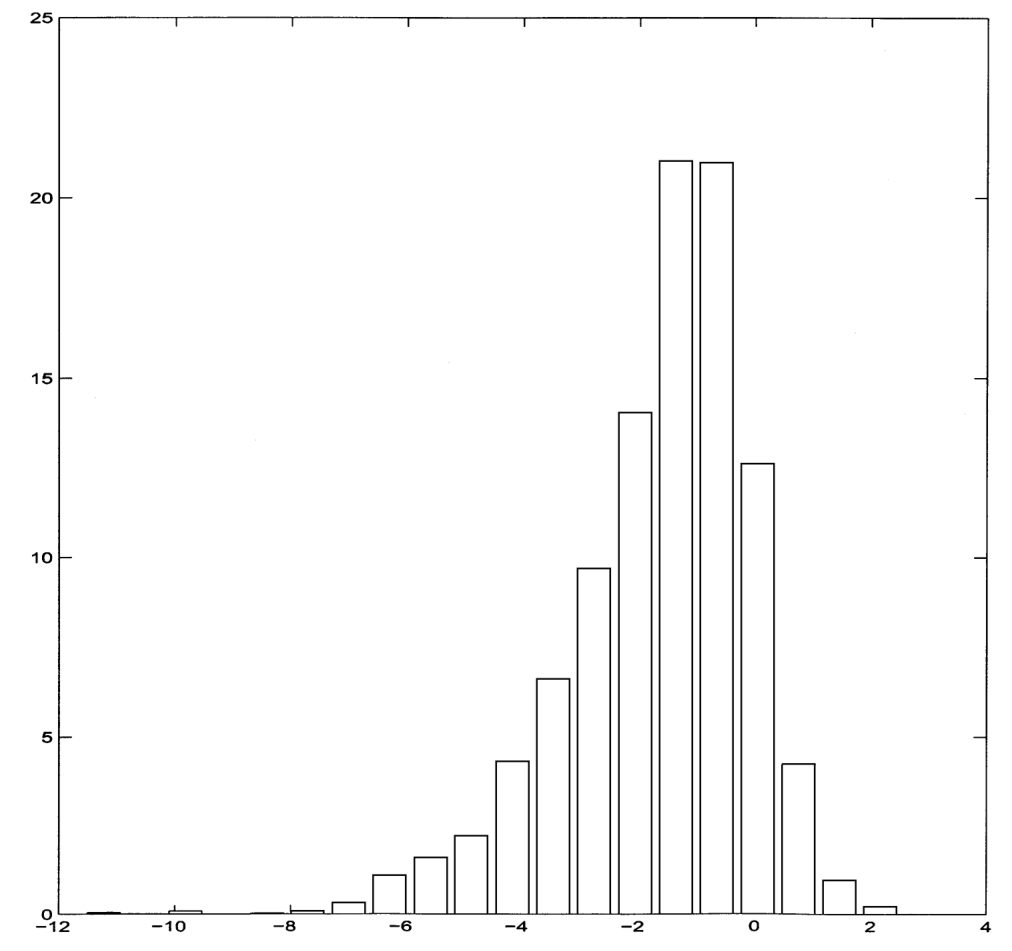
\includegraphics[width=\linewidth]{figures/ch08/nevo01_fig1_mushy.png}
\caption{Taste for sogginess (Mushy coefficient)}\label{fig:08-nevo-mushy}
\end{subfigure}\hfill
\begin{subfigure}[t]{0.48\linewidth}
\centering
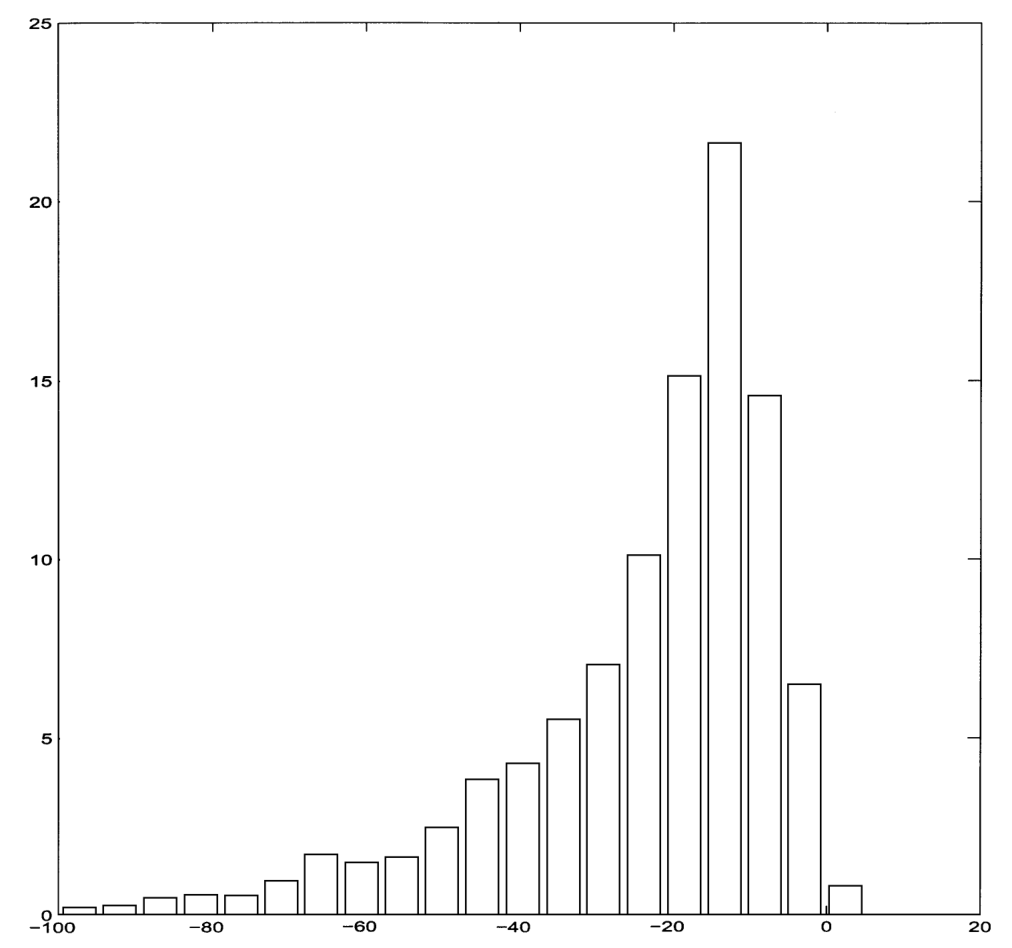
\includegraphics[width=\linewidth]{figures/ch08/nevo01_fig2_price.png}
\caption{Price coefficient}\label{fig:08-nevo-price}
\end{subfigure}
\caption{Frequency distributions of two individual coefficients implied by the estimates in
\cref{tab:08-nevo-full}. The horizontal axes give the value of the coefficient. The vertical axes, unlabeled
in the original, give frequencies. The bars sum to about 100, so the heights are percentages of simulated
consumers. Panel (a) puts about 15\% of consumers at a positive taste for sogginess. Panel (b) is skewed to the
left because it inherits the empirical distribution of demographics, and only 0.7\% of its mass lies above
zero.
Source: \citet{Nevo2001}, Figures 1 and 2.}
\label{fig:08-nevo-dists}
\end{figure}

The insignificance of the standard deviations says that the included demographics explain most of the
heterogeneity. The share of the variance of each coefficient explained by demographics exceeds 90\% (p.~330).
Appendix B of the paper re-estimates the model with the random shocks $\nu_i$ set to zero for the
characteristics that have demographic interactions. The estimates and margins barely change
(\cref{tab:08-nevo-robust}, column (i)). Nevo cautions against a stronger reading (p.~330, n.~26). The result
says that the data reject the assumed normal distribution for the unobserved part of tastes. It does not say
that information beyond demographics is useless. Purchase histories \citep{RossiMcCullochAllenby1996} and
second-choice data (the working-paper version of \citealp{BerryLevinsohnPakes2004}, \cref{sec:08-blp04}) do
reveal heterogeneity beyond demographics.

\casehead{Elasticities} \Cref{tab:08-nevo-elas} reproduces Table VII. Because elasticities vary across markets,
each entry is the median over the 1,124 markets of the elasticity of the row brand's share with respect to the
column brand's price. The own elasticities on the diagonal run from $-2.277$ (Cap'n Crunch) to $-4.252$
(Shredded Wheat). They are not ordered by price as the logit would require.

\begin{table}[htbp]
\centering
\caption{Median own- and cross-price elasticities of cereal demand}
\label{tab:08-nevo-elas}
\scriptsize
\setlength{\tabcolsep}{2.6pt}
\begin{tabular}{@{}rlrrrrrrrrrr@{}}
\toprule
 & & Corn & Frosted & Rice & Froot & & & Lucky & P Raisin & CapN & Shredded \\
\# & Brand & Flakes & Flakes & Krispies & Loops & Cheerios & Total & Charms & Bran & Crunch & Wheat \\
\midrule
1 & K Corn Flakes & $-$3.379 & 0.212 & 0.197 & 0.014 & 0.202 & 0.097 & 0.012 & 0.013 & 0.038 & 0.028 \\
2 & K Raisin Bran & 0.036 & 0.046 & 0.079 & 0.043 & 0.145 & 0.043 & 0.037 & 0.057 & 0.050 & 0.040 \\
3 & K Frosted Flakes & 0.151 & $-$3.137 & 0.105 & 0.069 & 0.129 & 0.079 & 0.061 & 0.013 & 0.138 & 0.023 \\
4 & K Rice Krispies & 0.195 & 0.144 & $-$3.231 & 0.031 & 0.241 & 0.087 & 0.026 & 0.031 & 0.055 & 0.046 \\
5 & K Frosted Mini Wheats & 0.014 & 0.024 & 0.052 & 0.043 & 0.105 & 0.028 & 0.038 & 0.054 & 0.045 & 0.033 \\
6 & K Froot Loops & 0.019 & 0.131 & 0.042 & $-$2.340 & 0.072 & 0.025 & 0.107 & 0.027 & 0.149 & 0.020 \\
7 & K Special K & 0.114 & 0.124 & 0.105 & 0.021 & 0.153 & 0.151 & 0.019 & 0.021 & 0.035 & 0.035 \\
8 & K Crispix & 0.077 & 0.086 & 0.114 & 0.034 & 0.181 & 0.085 & 0.030 & 0.037 & 0.048 & 0.043 \\
9 & K Corn Pops & 0.013 & 0.109 & 0.034 & 0.113 & 0.058 & 0.025 & 0.098 & 0.024 & 0.127 & 0.016 \\
10 & GM Cheerios & 0.127 & 0.111 & 0.152 & 0.034 & $-$3.663 & 0.085 & 0.030 & 0.037 & 0.056 & 0.050 \\
11 & GM Honey Nut Cheerios & 0.033 & 0.192 & 0.058 & 0.123 & 0.094 & 0.034 & 0.107 & 0.026 & 0.162 & 0.024 \\
12 & GM Wheaties & 0.242 & 0.169 & 0.175 & 0.025 & 0.240 & 0.113 & 0.021 & 0.026 & 0.050 & 0.043 \\
13 & GM Total & 0.096 & 0.108 & 0.087 & 0.018 & 0.131 & $-$2.889 & 0.017 & 0.017 & 0.029 & 0.029 \\
14 & GM Lucky Charms & 0.019 & 0.131 & 0.041 & 0.124 & 0.073 & 0.026 & $-$2.536 & 0.027 & 0.147 & 0.020 \\
15 & GM Trix & 0.012 & 0.103 & 0.031 & 0.109 & 0.056 & 0.026 & 0.096 & 0.024 & 0.123 & 0.016 \\
16 & GM Raisin Nut & 0.013 & 0.025 & 0.042 & 0.035 & 0.089 & 0.040 & 0.031 & 0.046 & 0.036 & 0.027 \\
17 & GM Cinnamon Toast Crunch & 0.026 & 0.164 & 0.049 & 0.119 & 0.089 & 0.035 & 0.102 & 0.026 & 0.151 & 0.022 \\
18 & GM Kix & 0.050 & 0.279 & 0.070 & 0.101 & 0.106 & 0.056 & 0.088 & 0.030 & 0.149 & 0.025 \\
19 & P Raisin Bran & 0.027 & 0.037 & 0.068 & 0.044 & 0.127 & 0.035 & 0.038 & $-$2.496 & 0.049 & 0.036 \\
20 & P Grape Nuts & 0.037 & 0.049 & 0.088 & 0.042 & 0.165 & 0.050 & 0.037 & 0.051 & 0.052 & 0.047 \\
21 & P Honey Bunches of Oats & 0.100 & 0.098 & 0.104 & 0.022 & 0.172 & 0.109 & 0.020 & 0.024 & 0.038 & 0.033 \\
22 & Q 100\% Natural & 0.013 & 0.021 & 0.046 & 0.042 & 0.103 & 0.029 & 0.036 & 0.052 & 0.046 & 0.029 \\
23 & Q Life & 0.077 & 0.328 & 0.091 & 0.114 & 0.137 & 0.046 & 0.096 & 0.023 & 0.182 & 0.029 \\
24 & Q CapN Crunch & 0.043 & 0.218 & 0.064 & 0.124 & 0.101 & 0.034 & 0.106 & 0.026 & $-$2.277 & 0.024 \\
25 & N Shredded Wheat & 0.076 & 0.082 & 0.124 & 0.037 & 0.210 & 0.076 & 0.034 & 0.044 & 0.054 & $-$4.252 \\
26 & Outside good & 0.141 & 0.078 & 0.084 & 0.022 & 0.104 & 0.041 & 0.018 & 0.021 & 0.033 & 0.021 \\
\bottomrule
\end{tabular}

\smallskip
\begin{minipage}{0.97\linewidth}
\footnotesize Notes: Entry $(i, j)$ is the percent change in the share of row brand $i$ for a one percent
change in the price of column brand $j$, as in \cref{eq:08-nevo-elas}. Each entry is the median over the 1,124
city-quarter markets. Own elasticities are negative numbers here, as in the paper. K, GM, P, Q and N denote
Kellogg, General Mills, Post, Quaker and Nabisco. Source: \citet{Nevo2001}, Table VII.
\end{minipage}
\end{table}

The substitution patterns follow characteristics. Lucky Charms, a children's cereal, is most sensitive to the
prices of other children's cereals (p.~330). It is least sensitive to the prices of Corn Flakes, Total and Wheaties, which
serve different segments.\footnote{Nevo names Corn Pops and Froot Loops as the brands to whose prices Lucky
Charms is most sensitive. Corn Pops and Wheaties are not among the ten columns printed in Table VII, so these
statements refer to the full matrix. Among the printed columns, row 14 is largest for Cap'n Crunch (0.147),
Frosted Flakes (0.131) and Froot Loops (0.124), and smallest for Corn Flakes (0.019).} The logit forces every
cross elasticity in a column to be equal. A summary of how far the estimates depart from that restriction is
the ratio of the largest to the smallest cross elasticity in a column, which equals one in the logit. The ratio
ranges from 21 for Corn Flakes to 3.5 for Shredded Wheat, with 95\% confidence intervals of 11 to 260 and 3
to 52 (p.~330). A low ratio also flags brands whose observed characteristics do not differentiate them well. A
formal test that all nonlinear parameters are zero, which is a specification test of the logit, is easily
rejected (p.~332, n.~28).

The last row gives the elasticity of the outside good's share with respect to each price. It is larger for
Corn Flakes (0.141) than for Froot Loops (0.022), in absolute terms and relative to the average cross elasticity
in each column (p.~332). Generic versions of Corn Flakes have larger shares than generic versions of Froot
Loops, and all generics belong to the outside good. A rise in the price of Corn Flakes therefore sends more
consumers to the outside option. Comparisons across columns should use semi-elasticities, because a one
percent price change differs in cents across brands (n.~29).

\subsection{Price-cost margins and the test of conduct}\label{sec:08-nevo01-margins}

\casehead{Predicted margins} \Cref{tab:08-nevo-margins} reproduces Table VIII and \cref{fig:08-nevo-margins}
plots it. Each entry is the median over the 27,862 observations of the margin implied by
\cref{eq:08-nevo-markup} under one ownership matrix. Medians are used to limit the influence of outliers, and
means with the 5\% tails trimmed are essentially identical (p.~332, n.~30). For the logit the computation is
analytical, using \eqref{eq:08-nevo-logit}. For the full model the confidence intervals come from 1,500
parametric bootstrap draws.

\begin{table}[htbp]
\centering
\caption{Median predicted price-cost margins under alternative conduct}
\label{tab:08-nevo-margins}
\footnotesize
\begin{tabular}{@{}lcc@{}}
\toprule
 & Logit & Full model \\
 & (\cref{tab:08-nevo-logit}, col.\ ix) & (\cref{tab:08-nevo-full}) \\
\midrule
Single-product firms & 33.6\% & 35.8\% \\
 & (31.8\%, 35.6\%) & (24.4\%, 46.4\%) \\
Current ownership of 25 brands & 35.8\% & 42.2\% \\
 & (33.9\%, 38.0\%) & (29.1\%, 55.8\%) \\
Joint ownership of 25 brands & 41.9\% & 72.6\% \\
 & (39.7\%, 44.4\%) & (62.2\%, 97.2\%) \\
Current ownership of all brands & 37.2\% & n.a. \\
 & (35.2\%, 39.4\%) & \\
Monopoly or perfect price collusion & 54.0\% & n.a. \\
 & (51.1\%, 57.3\%) & \\
\bottomrule
\end{tabular}

\smallskip
\begin{minipage}{0.84\linewidth}
\footnotesize Notes: Margins are $\frac{p - mc}{p}$, medians of the distribution over 27,862
brand-city-quarter observations. 95\% confidence intervals for the medians in parentheses, based on the
asymptotic distribution of the demand estimates. They are analytical for the logit and use 1,500 draws for the
full model. The last two rows require the shares of brands outside the sample, which suffice only for the
logit. Source: \citet{Nevo2001}, Table VIII.
\end{minipage}
\end{table}

\begin{figure}[htbp]
\centering
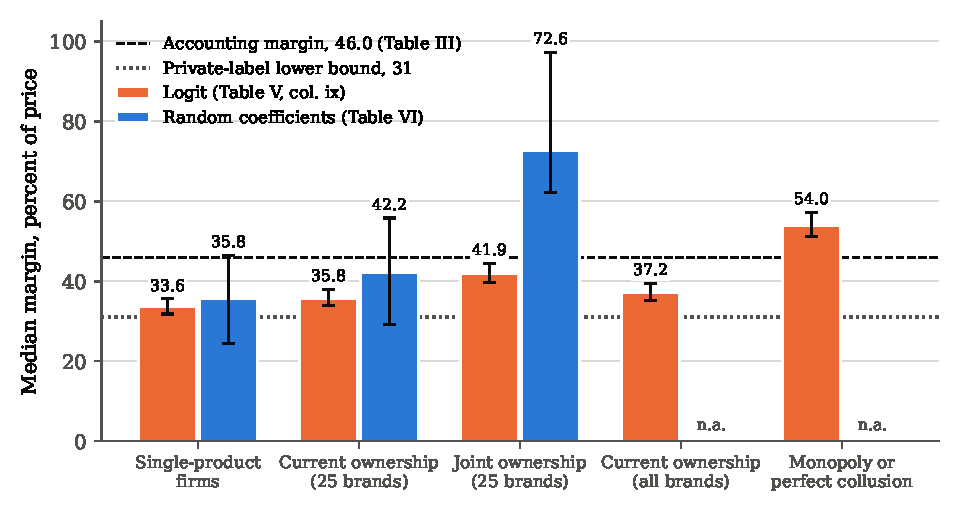
\includegraphics[width=0.97\linewidth]{figures/ch08/nevo01_margins.pdf}
\caption{Median predicted margins under five conduct models, with 95\% confidence intervals for the medians.
The dashed line is the accounting gross margin of 46.0\% of the retail price
(\cref{tab:08-nevo-costs}). The dotted line is the lower bound of about 31\% from the gap between national-brand
and private-label prices (p.~333). The random coefficients model predicts a joint-ownership margin far above
both lines, while its current-ownership interval covers them. The logit margins barely respond to ownership.
Redrawn from \citet{Nevo2001}, Table VIII.}
\label{fig:08-nevo-margins}
\end{figure}

The logit price coefficient, $-23.37$, is close to the full model's price coefficient in the Means column,
$-27.198$, yet their margins diverge as ownership widens. Under single-product pricing the medians are 33.6\% and 35.8\%. The portfolio effect adds 2.2
points in the logit and 6.4 points in the full model. Joint ownership of the 25 brands adds a further 6.1
points in the logit and 30.4 points in the full model. By \cref{prop:08-nevo-ownership}, these increments are
governed by the diversion ratios among co-owned brands. The full model concentrates diversion among similar
cereals, so joint pricing internalizes much more substitution.

The logit increments match \eqref{eq:08-nevo-logit} closely. In the logit the ratio of the joint-ownership
markup to the single-product markup of brand $j$ is $\frac{1-s_j}{1-S_{\mathcal{G}}}$. A rough calculation with
ratios of medians gives $\frac{41.9}{33.6} \approx 1.25$, which implies that the 25 brands hold about one fifth
of the potential market. Similarly $\frac{54.0}{33.6} \approx 1.61$ implies that all brands together hold
about 38\%. The ratio of the two, about one half, is consistent with the 43\% to 62\% of cereal volume that the
25 brands account for.\footnote{These are our calculations. A ratio of medians is not the median of the ratios,
and $s_j$ is treated as negligible, so the implied shares are approximations.}

\casehead{Observed margins} Testing requires a comparison with actual margins, which Nevo does not observe
directly. He treats the retail margin as an additional cost to manufacturers, which is consistent with many
models of manufacturer-retailer interaction (p.~333). The relevant observed margin is then the gross margin
relative to the retail price, 46.0\% from \cref{tab:08-nevo-costs}. This figure excludes promotional costs,
some of which, such as coupon rebates, are arguably marginal. Excluding them makes the observed margin a
generous one and the test conservative. Census data support the accounting figure. They are based on average
variable cost and give an upper bound.\footnote{The Census margin of 64.4\% is relative to the manufacturer's
price. On the retail-price basis of \cref{tab:08-nevo-costs}, Panel B, it corresponds to
$0.80 \times 64.4 \approx 51.5\%$. This conversion is ours.} A lower bound comes from the gap between the
prices of national brands and the corresponding private labels, about 31\% according to
\citet{Wongtrakool1994}. Private labels may carry a markup of their own and may have higher costs, so their
price exceeds the national brands' marginal cost and the gap understates the margin (pp.~333--334). Nevo
cautions that accounting margins are crude \citep{FisherMcGowan1983} and uses them only to discriminate
between models.

\casehead{The test} The predicted margins differ enough that even crude observed margins separate the models
(p.~334). The joint-ownership interval for the full model, 62.2\% to 97.2\%, lies above both the typical margin
of 46.0\% and the lower bound of 31\%. Joint profit maximization over the 25 brands is therefore rejected. The
current-ownership interval, 29.1\% to 55.8\%, contains both figures, so multi-product Nash-Bertrand pricing is
not rejected. The decomposition implied by the full model's medians attributes about 85\% of the
current-ownership margin to differentiation ($\frac{35.8}{42.2}$) and the remaining 6.4 points to the
portfolio effect.

Two further arguments strengthen the conclusion. The first concerns the restriction to 25 brands (p.~334). The
price coefficient should not be biased by the selection, and estimates on other samples confirm this. Brands
outside the sample are probably more elastic, which would lower the single-product margins. Weighting by
market shares, which is the likely effect of including small brands, offsets this. The share-weighted means
are roughly 2 to 3 points above the medians in Table VIII. For the current-ownership and collusive models a second force operates. Moving products from the
outside good into the inside set raises the predicted margins, and the effect grows with the number of jointly
priced products. Adding brands would therefore move the Nash-Bertrand prediction closer to the observed margins
and the collusive prediction further away. In this sense Table VIII is conservative.

The second argument concerns the logit. Applied to the logit column, the same test would not reject full
collusion over all products (p.~335). The logit's collusive margins, 41.9\% for the 25 brands and 54.0\% for
all brands, lie close to the observed margin of 46.0\%. Nevo stresses that this result is driven entirely by the logit's restrictive
substitution patterns and says nothing about conduct. It is the clearest demonstration in the paper of why
flexible substitution patterns matter for questions of market power.

\casehead{Why not a formal test} Nevo explains why he does not use two alternatives (pp.~334--335). One is to
estimate a conduct parameter, as in homogeneous-goods industries \citep{Bresnahan1989}. Its interpretation is
problematic \citep{Corts1999}, and its identification requirements are unlikely to be met with differentiated
products \citep{Nevo1998}. The other is a non-nested test of fully specified models
\citep{Bresnahan1987,GasmiLaffontVuong1992}. That requires the likelihood of each model, hence distributional
assumptions on the errors and a complete supply equation, and there is no natural set of such assumptions.
\Cref{ch:conduct} and \cref{sec:08-supply} discuss conduct testing more generally.

\subsection{Robustness*}\label{sec:08-nevo01-robust}

Appendix B of the paper reports four alternative specifications of the full model, reproduced in condensed form
in \cref{tab:08-nevo-robust}. Column (i) drops the random shocks $\nu_i$ for the characteristics that interact
with demographics. Its price coefficient ($-25.595$) and margins (36.1\%, 41.9\% and 67.4\%) are close to the
preferred ones, which supports the claim that demographics drive the heterogeneity. Columns (ii) and (iii) are
nonlinear least squares without instruments, without and with brand dummies. Their price coefficients are
$-4.291$ and $-7.407$. The implied margins are absurd. They range from 67.6\% to 84.5\% under Nash-Bertrand
pricing, and above 100\% under collusion. Column (iv) uses brand dummies as instruments, the analogue of
characteristic-based identification. Its estimates are imprecise and 22.4\% of its price coefficients are
positive. Nevo notes that it lacks the variance-reduction methods of BLP (p.~339).

\begin{table}[htbp]
\centering
\caption{Alternative specifications of the full model}
\label{tab:08-nevo-robust}
\footnotesize
\begin{tabular}{@{}lrrrr@{}}
\toprule
 & (i) & (ii) & (iii) & (iv) \\
 & No $\nu_i$ on & NLLS, no & NLLS, brand & GMM, brand \\
 & interacted chars. & brand dummies & dummies & dummies as IVs \\
\midrule
Mean price coefficient & $-$25.595 & $-$4.291 & $-$7.407 & $-$9.856 \\
 & (2.673) & (0.143) & (0.164) & (3.039) \\
Price $\times$ income & 311.101 & 34.565 & 8.552 & 21.575 \\
 & (61.797) & (1.455) & (0.974) & (96.912) \\
Percent of price coefficients $>0$ & 0 & 16.1 & 0 & 22.4 \\
\addlinespace
Single-product margin & 36.1\% & 67.6\% & 75.7\% & 48.2\% \\
Multi-product margin & 41.9\% & 75.6\% & 84.5\% & 54.0\% \\
Collusive margin & 67.4\% & 103.9\% & 117.6\% & 88.9\% \\
\bottomrule
\end{tabular}

\smallskip
\begin{minipage}{0.88\linewidth}
\footnotesize Notes: Standard errors in parentheses. 27,862 observations. NLLS is nonlinear least squares,
which does not instrument for price. Column (i) is the preferred specification without $\nu_i$ for the
characteristics that have demographic interactions. The paper also reports all taste parameters, omitted here.
The preferred specification gives 35.8\%, 42.2\% and 72.6\% (\cref{tab:08-nevo-margins}). Source:
\citet{Nevo2001}, Table B(II).
\end{minipage}
\end{table}

Other checks point the same way (pp.~327, 335--336). A specification with city fixed effects, the analogue of
column (x) of \cref{tab:08-nevo-logit}, gives point estimates close to the preferred ones but very large
standard errors. This is expected, since demographics barely change within a city over five years. A
multi-stage budgeting demand system in the style of \citet{HausmanLeonardZona1994} and \citet{Hausman1997},
covered in \cref{ch:aids}, shows interesting differences in cross-price substitution but the same conclusions
about conduct. Studies based on household data, a random coefficients model by \citet{Kiser1996} and a nested
logit by \citet{Shum1999}, use different data and different identifying assumptions. They produce very similar
own- and cross-price elasticities.

\subsection{Interpretation, limitations and contribution}\label{sec:08-nevo01-assess}

\casehead{Interpretation} If Nash-Bertrand pricing is the benchmark of noncollusive behavior, prices in RTE
cereal are not collusive, even with margins above 45\% (p.~336). High margins reflect consumers' willingness
to pay for their favorite brands and firms' internalization of substitution within their portfolios. To the
extent that the industry has market power, it lies in the ability to maintain a portfolio of differentiated
brands and to shape perceived quality through advertising. Nevo relates this to the FTC case. The standard
account of the complaint mentions cooperative pricing, but its core was brand proliferation as a barrier to
entry \citep{Schmalensee1978}. In this sense the FTC focused on the dimensions of competition that Nevo finds
important. His model, however, takes brands and advertising as given and cannot evaluate their competitive
effects (p.~336).

\casehead{Limitations} The test rules out only the extreme form of cooperation, joint maximization of profits
over all 25 brands. Cooperation within a subset of products or firms, such as two raisin brans or two smaller
producers, is not tested and would require more detailed cost data (p.~336). The observed margin is a single
accounting figure for a typical Kellogg brand, compared with medians over brands, cities and quarters. The
Hausman instruments rest on independence of demand shocks across cities, which overidentification tests reject
in the logit unless city effects are added. Advertising is treated as exogenous, and its implied elasticity is
implausibly low. The model is static and uses quarterly averages of prices that include temporary promotions.
The standard deviations of the random coefficients are imprecise because the choice set barely varies. The
full model's margins have wide confidence intervals. The single-product interval runs from 24.4\% to 46.4\%.
Finally, the definition of the potential market as one serving per person per day fixes the outside share,
and with it the level of the implied markups (\cref{sec:08-model}).

\casehead{Contribution} The paper made four contributions that became standard. It combined brand fixed effects
with the BLP estimator and recovered taste means by minimum distance, so that price endogeneity due to $\xi_j$
needs no instrument. It used prices in other markets as instruments in a random coefficients model and checked
them against cost proxies. It modeled heterogeneity with the empirical distribution of demographics. Above all,
it turned the supply side into a tool for measuring conduct. Comparing margins implied by alternative ownership
matrices with observed margins gives a transparent decomposition of market power. The same model and data
underlie the merger simulations of \citet{Nevo2000b}, discussed in \cref{ch:mergers}. Hausman's valuation of a
new cereal brand, discussed in \cref{ch:newgoods}, depends on the same kind of assumption about price
competition that Nevo tests. Later work uses the demand elasticities to discriminate between models of conduct
in the same industry, including common-ownership pricing \citep{BackusConlonSinkinson2021}.

\begin{table}[htbp]
\centering
\caption{Identification and counterfactual map of Nevo (2001)}
\label{tab:08-nevo01-map}
\footnotesize
\renewcommand{\arraystretch}{1.1}
\begin{tabularx}{\textwidth}{@{}>{\raggedright\arraybackslash}p{2.6cm}>{\raggedright\arraybackslash}X@{}}
\toprule
Observed data & IRI scanner prices and servings of 25 cereal brands in up to 65 cities, quarterly from 1988 to
  1992 (27,862 brand-city-quarters). Brand characteristics, national advertising, CPS demographic draws, and
  accounting margins for a typical brand. \\
\addlinespace
Latent objects & City-quarter quality deviations $\tilde\xi_{jt}$, consumer tastes $\nu_i$, marginal costs
  and markups. \\
\addlinespace
Estimated parameters & The price and advertising coefficients, brand and quarter effects, demographic
  interactions $\Pi$ and standard deviations $\Sigma$. Taste means come from a minimum-distance step. \\
\addlinespace
Identifying variation & Prices of the same brand in other cities of the region, checked against cost
  proxies. Brand effects absorb national quality, and cross-city differences in demographics identify $\Pi$. \\
\addlinespace
Maintained assumptions & City demand shocks are independent across cities after brand, time and demographic
  controls, and costs share a regional component. Static pricing, exogenous advertising, and a potential
  market of one serving per person per day. \\
\addlinespace
Counterfactual and what it holds fixed & Margins implied by \eqref{eq:08-nevo-markup} under single-product,
  current and joint ownership, at observed prices and shares. Demand is held at its estimates, and only the
  ownership matrix changes. \\
\addlinespace
Conclusion & Current ownership predicts a median margin of 42.2 percent, whose interval contains the
  observed margins. Joint ownership of the 25 brands predicts 72.6 percent and is rejected. Margins come
  from differentiation and portfolios, given the Hausman instruments. \\
\addlinespace
One limitation & Only joint profit maximization over all 25 brands is tested. Collusion within a subset of
  brands or firms is not. \\
\addlinespace
Source and our additions & The tables are Nevo's. \Cref{prop:08-nevo-ownership}, the advertising
  benchmark and the logit share calculations behind the margin ratios are ours. \\
\addlinespace
Tools in the appendices & \Cref{sec:A-iv,sec:A-gmm,sec:A-delta-boot}. \\
\bottomrule
\end{tabularx}
\end{table}

\section{Case study: Berry, Levinsohn and Pakes (2004), micro and macro data}\label{sec:08-blp04}

\citet{BerryLevinsohnPakes2004}, henceforth BLP (2004), return to the automobile market with a new kind of
data. A proprietary survey by General Motors covers a large sample of 1993 new-vehicle buyers. It records
each buyer's demographics, the vehicle bought and the vehicle the buyer would have bought had the first choice
been unavailable. The paper asks what such consumer-level data, and second choices in particular, add to the
identification of substitution patterns. The answer has three parts. Second choices pin down the parameters
that govern substitution. Unobserved heterogeneity in tastes is needed to match them, even with rich
demographics. A single cross section still cannot determine the level of price elasticities. The general
estimator was introduced in \cref{sec:08-micro}. Here we follow the paper in detail, and
\cref{tab:08-blp04-map} at the end of the section maps it. Page numbers refer to the
journal article.\footnote{BLP (2004) write observed household attributes as $z_{ir}$, the coefficients on
their interactions with characteristics as $\beta^{o}_{kr}$ (``observed'') and the standard deviations of
unobserved tastes as $\beta^{u}_k$ (``unobserved''). We write $D_{ir}$, $\pi_{kr}$ and $\sigma_k$, so that
$\beta^{o}$ and $\beta^{u}$ correspond to the matrices $\Pi$ and $\Sigma$ of \cref{sec:08-model}.}

\subsection{The question}\label{sec:08-blp04-question}

We abbreviate \citet{BerryLevinsohnPakes1995}, the subject of \cref{sec:08-blp95}, as BLP (1995). In that
paper, substitution patterns are identified from changes across markets and years in the choice set and in the
distribution of consumer attributes. The distribution of tastes,
conditional on observed incomes, is assumed to be stable over time (pp.~69--70). Earlier discrete choice work,
and \citet{Goldberg1995} and \citet{Petrin2002} in industrial organization, matched consumer attributes to
choices. Such data identify substitution to the extent that observed attributes explain it.
\Cref{sec:08-goldberg} discusses Goldberg's study.

Second-choice data offer a different source of identification (p.~70). They give a direct, data-based measure
of substitution, so one can ask which models reproduce it. By requiring the parameters to match observed
second choices, the econometrician gains identifying power that does not rely on exogenous changes in choice
sets. The paper also stresses a limit. Second choices in a single cross section, with one price per vehicle,
reveal the pattern of substitution but not the level of price elasticities. Outside information must fix the
level. The paper closes with two out-of-sample predictions, the introduction of luxury sport utility vehicles
and the closure of the Oldsmobile division of General Motors.

\subsection{Data}\label{sec:08-blp04-data}

\casehead{The CAMIP survey} The consumer data come from a proprietary survey conducted for General Motors,
here called CAMIP (pp.~79--80). It samples from the registrations of 1993 model-year vehicles of all
manufacturers, not only GM. For each vehicle a given number of buyers is sampled, so the design is a random
sample conditional on the vehicle purchased. A sample of this kind is called \emph{choice-based}. The subsample
used has 37,500 observations. The questionnaire asks about income, age of the household head, family size and
place of residence, and each question is matched to a question in the CPS.

\Cref{tab:08-blp04-samples} compares CAMIP households with CPS households. CAMIP over-represents high incomes.
Only 6.52\% of CPS households earn \$85,000 or more, against 25.13\% of CAMIP households, and mean income is
\$72,270 in CAMIP against \$34,170 in the CPS. New-vehicle buyers are richer than the population. More
surprisingly, CAMIP households are less urban (35\% against 46\%) and more rural (35\% against 25\%).
Rural households buy a disproportionate number of vehicles, which helps explain the high share of trucks
(p.~80).

\begin{table}[htbp]
\centering
\caption{CPS and CAMIP household samples}
\label{tab:08-blp04-samples}
\footnotesize
\begin{tabular}{@{}lrrrr@{}}
\toprule
Income range (\$) & Percent in CPS & Percent in CAMIP & CPS group mean & CAMIP group mean \\
\midrule
0--36,500 & 64.17 & 25.00 & 16.90 & 25.96 \\
36,500--55,000 & 16.97 & 23.16 & 44.89 & 45.43 \\
55,000--85,000 & 12.34 & 26.71 & 66.93 & 67.46 \\
85,000 and above & 6.52 & 25.13 & 114.25 & 148.19 \\
All & 100.00 & 100.00 & 34.17 & 72.27 \\
\midrule
Other demographics & & & CPS mean & CAMIP mean \\
\midrule
Family size & & & 2.36 & 2.65 \\
Age of household head & & & 46.80 & 46.18 \\
Number of kids & & & 0.66 & 0.58 \\
Urban & & & 0.46 & 0.35 \\
Rural & & & 0.25 & 0.35 \\
Suburban & & & 0.29 & 0.30 \\
\bottomrule
\end{tabular}

\smallskip
\begin{minipage}{0.86\linewidth}
\footnotesize Notes: Group means of income in thousands of dollars. Source:
\citet{BerryLevinsohnPakes2004}, Table 1.
\end{minipage}
\end{table}

\casehead{The choice set and product data} The vehicle list follows GM's sampling cells and has 203 vehicles:
147 cars, 25 sport utility vehicles (SUVs), 17 vans and 14 pickup trucks (p.~81). Early runs used 218
vehicles. The final runs aggregate 15 very expensive vehicles, with an average price of \$74,000 and a combined
share of 0.3\% of vehicles sold, into one ``super-luxury'' model (n.~9). The survey records transaction prices.
Characteristics are those of the modal vehicle in each cell, the most commonly purchased combination of
options, and price is the average price of that modal vehicle. About 10.6 million vehicles were sold in 1993
at an average price of \$18,500, for total sales of about \$196 billion. The continuous characteristics are horsepower
per weight (HP), number of passengers (Pass, a measure of size), city miles per gallon (MPG) and number of power
accessories (Acc). They also include safety features (Safe, antilock brakes plus airbags) and the payload of
light trucks. The
dummies mark minivans, SUVs, pickups, full-size vans, sports cars and four- or all-wheel drive (Allw). The interactions
PUPayl and SUVPayl multiply payload by the pickup and SUV dummies (Table 2).

\casehead{Demographic patterns} Means of vehicle characteristics by demographic group reveal clear interactions
(p.~81). Examples are kids with minivans, income with price, rural residence with pickups and four-wheel drive,
and age with nearly everything. The authors used such tables to choose the interactions in utility.
\Cref{tab:08-blp04-groups} condenses their Table 4. The mean price of the vehicle chosen rises from \$16,600 in
the lowest income group to \$26,300 in the highest. Households with two or more children choose a minivan 18\% of
the time, against 3\% for households without children. The mean of PUPayl, the pickup dummy times payload in
thousands of pounds, is 0.31 among rural households, against 0.14 among urban and 0.10 among suburban households. Buyers over 50 choose vehicles that are more
expensive and larger, with more accessories, and they rarely choose sports cars or SUVs (0.07 and 0.04).

\begin{table}[htbp]
\centering
\caption{Mean characteristics of the vehicles chosen by demographic group in the CAMIP data (condensed)}
\label{tab:08-blp04-groups}
\footnotesize
\setlength{\tabcolsep}{4.5pt}
\begin{tabular}{@{}lrrrrrrrrrr@{}}
\toprule
Group & Price & HP & Pass & Acc & Sport & MPG & Allw & Miniv & SUV & PUPayl \\
\midrule
\multicolumn{11}{@{}l}{\textit{Age of household head}} \\
\quad 30 or less & 16.6 & 4.7 & 4.5 & 2.6 & 0.20 & 22.0 & 0.13 & 0.03 & 0.15 & 0.24 \\
\quad 30--50 & 20.1 & 4.8 & 4.9 & 3.1 & 0.15 & 20.4 & 0.13 & 0.08 & 0.13 & 0.18 \\
\quad Over 50 & 22.4 & 4.9 & 5.1 & 3.4 & 0.07 & 19.8 & 0.06 & 0.04 & 0.04 & 0.19 \\
\multicolumn{11}{@{}l}{\textit{Number of children}} \\
\quad 0 & 20.9 & 4.9 & 4.8 & 3.2 & 0.14 & 20.4 & 0.10 & 0.03 & 0.09 & 0.20 \\
\quad 1 & 19.2 & 4.7 & 4.8 & 3.0 & 0.13 & 21.0 & 0.12 & 0.06 & 0.11 & 0.20 \\
\quad 2 or more & 20.1 & 4.6 & 5.3 & 3.1 & 0.08 & 19.9 & 0.12 & 0.18 & 0.13 & 0.16 \\
\multicolumn{11}{@{}l}{\textit{Residence}} \\
\quad Urban & 20.6 & 4.8 & 4.9 & 3.2 & 0.13 & 20.7 & 0.10 & 0.05 & 0.10 & 0.14 \\
\quad Suburban & 21.7 & 5.0 & 4.9 & 3.4 & 0.15 & 20.3 & 0.10 & 0.06 & 0.10 & 0.10 \\
\quad Rural & 19.2 & 4.7 & 4.9 & 3.0 & 0.11 & 20.2 & 0.12 & 0.06 & 0.11 & 0.31 \\
\multicolumn{11}{@{}l}{\textit{Household income (\$)}} \\
\quad 37,000 or less & 16.6 & 4.6 & 4.8 & 2.6 & 0.12 & 21.9 & 0.08 & 0.04 & 0.07 & 0.25 \\
\quad 37,000--55,000 & 18.5 & 4.7 & 4.9 & 3.0 & 0.12 & 20.7 & 0.10 & 0.07 & 0.10 & 0.24 \\
\quad 55,000--85,000 & 20.3 & 4.8 & 4.9 & 3.2 & 0.14 & 20.0 & 0.13 & 0.07 & 0.13 & 0.19 \\
\quad Over 85,000 & 26.3 & 5.2 & 4.9 & 3.7 & 0.14 & 19.1 & 0.11 & 0.05 & 0.12 & 0.08 \\
\bottomrule
\end{tabular}

\smallskip
\begin{minipage}{0.95\linewidth}
\footnotesize Notes: Price in thousands of dollars. Sport, Allw, Miniv and SUV are shares of vehicles with the
attribute. PUPayl is the pickup dummy times payload in thousands of pounds. The original table also reports
safety features, the van dummy, SUV payload and rows by family size. Source: \citet{BerryLevinsohnPakes2004},
Table 4 (p.~84).
\end{minipage}
\end{table}

\casehead{Second choices}
\Cref{tab:08-blp04-second} reproduces the second-choice information for 17 representative vehicles. The 166
sampled buyers of the Ford Escort named the Ford Tempo most often (16 buyers), followed by the Ford Taurus.
Together these two account for 18\% of Escort buyers, who named 53 different second choices in all (p.~86).
Second choices are more concentrated for light trucks and expensive cars. They are often made by the same
company as the first choice, which supports pricing that maximizes the joint profits of each firm's products.

\begin{table}[htbp]
\centering
\caption{Examples of second choices in the CAMIP data}
\label{tab:08-blp04-second}
\footnotesize
\setlength{\tabcolsep}{4pt}
\begin{tabular}{@{}lrlrlrr@{}}
\toprule
 & & Modal second & Number & Next second & (Modal $+$ & Different \\
First choice & $n_j$ & choice & choosing & choice & next)$\,\div\, n_j$ & choices \\
\midrule
Metro & 188 & Escort & 22 & Geo Storm & .22 & 49 \\
Cavalier & 238 & Escort & 16 & LeBaron & .12 & 59 \\
Escort & 166 & Tempo & 16 & Taurus & .18 & 53 \\
Corolla & 250 & Civic & 42 & Camry & .33 & 55 \\
Sentra & 203 & Corolla & 34 & Civic & .31 & 60 \\
Accord & 223 & Camry & 58 & Taurus & .35 & 61 \\
Taurus & 147 & Camry & 18 & Sable & .22 & 45 \\
Legend & 119 & Lexus ES300 & 19 & Lexus SC300 & .24 & 40 \\
Seville & 243 & DeVille & 38 & Lincoln MK8 & .26 & 49 \\
Lexus LS400 & 148 & DeVille & 33 & Infiniti Q45 & .39 & 27 \\
Caravan & 166 & Voyager & 31 & Aerostar & .32 & 36 \\
Quest & 232 & Caravan & 50 & Villager & .43 & 31 \\
Grand Cherokee & 137 & Explorer & 75 & Blazer & .59 & 34 \\
Trooper & 137 & Explorer & 43 & Rodeo & .41 & 27 \\
GMC full-size pickup & 469 & Chevy full-size pickup & 222 & Ford full-size pickup & .55 & 29 \\
Toyota pickup & 113 & Ford Ranger & 29 & Nissan pickup & .43 & 25 \\
Econovan & 90 & Chevy full-size van & 20 & Suburban & .44 & 23 \\
\bottomrule
\end{tabular}

\smallskip
\begin{minipage}{0.92\linewidth}
\footnotesize Notes: $n_j$ is the number of CAMIP buyers of the first-choice vehicle. The sixth column is the
fraction of them whose second choice is either the modal or the next most common second choice. Source:
\citet{BerryLevinsohnPakes2004}, Table 5.
\end{minipage}
\end{table}

Second choices resemble first choices. Across households, the correlations between the characteristics of the
first and the second choice are all positive and highly significant (p.~86). They are about 0.7 for price and
the minivan dummy, about 0.6 for MPG, size and the other type dummies, and between 0.3 and 0.5 for the rest.
The survey does not ask whether the household would have bought a vehicle at all. The data therefore say
nothing directly about substitution to the outside good.

\subsection{The model}\label{sec:08-blp04-model}

Households $i$ choose among vehicles $j = 1,\dots,J$ and the outside option $j = 0$. Let $k$ index observed
characteristics, including price, and $r$ index observed household attributes. Utility is linear in
characteristics (BLP 2004, equations (1) and (2)):
\begin{equation}\label{eq:08-blp04-utility}
u_{ij} = \sum_k x_{jk}\beta_{ik} + \xi_j + \epsilon_{ij},
\qquad
\beta_{ik} = \bar\beta_k + \sum_r D_{ir}\pi_{kr} + \sigma_k\nu_{ik} .
\end{equation}
The idiosyncratic shocks $\epsilon_{ij}$ are i.i.d.\ type-I extreme value, and the $\nu_{ik}$ are independent
standard normals. Substituting the taste equation into utility gives (equations (3) and (4))
\begin{equation}\label{eq:08-blp04-delta}
u_{ij} = \delta_j + \sum_{k,r} x_{jk}D_{ir}\pi_{kr} + \sum_k x_{jk}\nu_{ik}\sigma_k + \epsilon_{ij},
\qquad
\delta_j = \sum_k x_{jk}\bar\beta_k + \xi_j .
\end{equation}
The model has one unobserved product characteristic, valued equally by all households. The authors note that
this simplifies computation but is not essential to their arguments (p.~71, n.~3).

\casehead{Price and income} Price receives special treatment (p.~87). The household-specific part of the
price coefficient is $-e^{-W_i}$, where $W_i$ is ``effective wealth,''
\begin{equation}\label{eq:08-blp04-wealth}
W_i = \sum_r D_{ir}\pi_{wr} + \sigma_w\nu_{iw} .
\end{equation}
The common part of the price coefficient, $\bar\beta_p$, sits in $\delta_j$ by \cref{eq:08-blp04-delta}.
Write $\bar\alpha = -\bar\beta_p$. Household $i$'s price sensitivity is then
\begin{equation}\label{eq:08-blp04-alpha}
\alpha_i = \bar\alpha + e^{-W_i}.
\end{equation}
Because $e^{-W_i} > 0$, no household with $\bar\alpha \geq 0$ prefers higher prices, which is the reason for the
exponential form. The factor $e^{-W_i}$ is lognormal given demographics. The attributes in $W_i$ are a constant,
family size and a spline in income. Preliminary runs allowed the slope of the spline to change at each quartile
of the CAMIP income distribution, but only a change at the 75th percentile was needed. Higher income raises
$W_i$ and lowers price sensitivity.

\casehead{The outside good} Little is known a priori about the value of not buying. Early runs let it depend
linearly on all household attributes plus a normal disturbance. Only income, family size and sometimes the
number of adults mattered (p.~87). The normal disturbance on the outside good plays the role of a random
coefficient on the inside-good constant (\cref{sec:08-model}).

\casehead{What micro data identify} Equation \eqref{eq:08-blp04-delta} is a random coefficients discrete
choice model with a separate constant $\delta_j$ for each product. Given parametric assumptions on
$(\nu,\epsilon)$, the micro data identify $(\delta, \Pi, \Sigma)$ without any assumption on the joint
distribution of $(\xi, x)$ (pp.~72--73). Some questions, such as ideal price indices, need only these
parameters. Elasticities, however, also require the effect of price on $\delta_j$, that is, $\bar\beta_p$. The
equation $\delta_j = \sum_k x_{jk}\bar\beta_k + \xi_j$ has only $J$ observations, and price is correlated with
$\xi_j$. Identifying $\bar\beta$ therefore requires an assumption on $(\xi, x)$, the same identification
problem as in BLP (1995). Micro data solve one part of the problem, the substitution parameters, and leave the
other part untouched. \citet{BerryHaile2024}, discussed in \cref{sec:08-micro}, generalize this division of
labor nonparametrically.

Aggregate demand integrates over the distribution $P_w$ of household attributes $w_i = (D_i, \nu_i,
\epsilon_i)$ (equation (5)):
\[
s_j(\delta, \Pi, \Sigma; x, P_w) = \int_{A_j(\delta, \Pi, \Sigma; x)} P_w(\dd w),
\qquad A_j = \Big\{w : \max_{r = 0,\dots,J} u_{ir}(w) = u_{ij}\Big\}.
\]
Conditional on $(D_i, \nu_i)$, the logit form gives the choice probability (equation (6))
\begin{equation}\label{eq:08-blp04-prob}
\Pr(j^{(1)}_i = j \mid D_i, \nu_i, \theta) =
\frac{\exp\big(\delta_j + \sum_{k,r}x_{jk}D_{ir}\pi_{kr} + \sum_k x_{jk}\nu_{ik}\sigma_k\big)}
{1 + \sum_q \exp\big(\delta_q + \sum_{k,r}x_{qk}D_{ir}\pi_{kr} + \sum_k x_{qk}\nu_{ik}\sigma_k\big)},
\end{equation}
where $\theta = (\delta, \Pi, \Sigma)$ and $j^{(1)}_i$ denotes household $i$'s first choice.

\subsection{The estimator}\label{sec:08-blp04-estimator}

Maximum likelihood is efficient but was too burdensome, so the authors use a method of moments estimator
(p.~74). It matches three sets of moments (p.~75).
\begin{enumerate}
\item \emph{First-choice moments.} Covariances between the characteristics of the vehicle bought and the
attributes of the household, for example family size and vehicle size. They identify $\Pi$. The means of
household attributes among buyers identify the parameters of the outside good, because CAMIP samples vehicles
roughly in proportion to their shares.
\item \emph{Second-choice moments.} Covariances between the characteristics of the first and the second
choice, one for each characteristic with a random coefficient. They identify $\Sigma$. If $\Sigma = 0$, the
observed attributes alone determine both choices and hence their correlation. A predicted correlation far below
the observed one signals that unobserved tastes matter.
\item \emph{Market shares} of the $J$ products, which identify $\delta$.
\end{enumerate}
A footnote makes the role of interactions precise (p.~75, n.~5). If $\Pi = 0$ and only first choices were
used, aggregate shares would be sufficient statistics for the first-choice data. Matching individuals to their
vehicles would then add no information.

\casehead{Concentrating out the product constants} With over 200 vehicles, $\delta$ has over 200 elements and
the full parameter vector about 250 (p.~77). The authors exploit the precision of the aggregate shares. The
observed share vector $s^N$, computed from $N$ households (over 100 million), is multinomial around the true
$s(\delta_0, \beta_0)$ with variance of order $N^{-1}$. An efficient estimator therefore sets predicted shares
equal to observed shares. Let $\theta_2 = (\Pi, \Sigma)$, which BLP (2004) call $\beta$. For each trial value of
$\theta_2$, the contraction of \cref{sec:08-inversion} finds the $\delta^{n_s,N}(\theta_2)$ that solves the simulated
share equations \eqref{eq:08-blp04-shares} (their equation (7)). The pairs $(D_r, \nu_r)$ combine a CPS draw of
demographics with a draw of $\nu$. They are drawn once and held fixed, as \citet{PakesPollard1989} require. Importance
sampling as in BLP (1995) reduces simulation variance (p.~77, n.~6). The micro moments are then evaluated at
$(\theta_2, \delta^{n_s,N}(\theta_2))$, and the search runs over $\theta_2$ alone.

\casehead{First-choice moments and Bayes' rule} Because the sample is choice-based, the model's prediction to
be matched is the expected attribute of a household that chose a given vehicle. Let $n_j$ be the number of
sampled buyers of $j$ and $n = \sum_j n_j$. The first-choice moments \eqref{eq:08-blp04-g1} (their equation (8))
compare the sample mean attribute of $j$'s buyers with its model counterpart, one moment for each interaction in
utility. The model counterpart is the Bayes formula \eqref{eq:08-bayes} (their equation (9)). By construction of
$\delta^{n_s,N}(\theta_2)$, its denominator equals $s^N_j$, and its numerator is simulated with the same draws as the
shares, as in \eqref{eq:08-bayes-sim} (their equation (10)). The approach follows the literature on choice-based
sampling \citep{ManskiLerman1977,ImbensLancaster1994}. The same structure underlies the micro moments of
\citet{Petrin2002} in \cref{ch:newgoods}.

\casehead{Second-choice probabilities} The second-choice moments require the probability that a household
whose first choice is $j$ names $q$ as its second choice. The survey asks for a second vehicle, so both $j$
and the outside good leave the choice set. By \cref{lem:08-blp04-second}, conditional on $(D_i, \nu_i)$ the
probability is again a logit with $j$ and the outside good removed from the denominator (p.~79). It equals
$\Pr(j^{(2)}_i = q \mid j^{(1)}_i = j, D_i, \nu_i, \theta_2) = \frac{\exp(V_{iq})}{\sum_{l \neq 0, j}\exp(V_{il})}$,
where $V_{il}$ is the deterministic utility in \eqref{eq:08-blp04-prob}. The individual second choice satisfies IIA, but
the aggregate one does not, because the integral over $(D,\nu)$ weights each household by its probability of having
chosen $j$ first, as in \eqref{eq:08-second-agg}. Buyers of $j$ have tastes favorable to $j$'s characteristics and pick
second choices with similar characteristics. The second-choice moment for characteristic $k$ starts from the average
$x_k$ of the second choices named by $j$'s buyers. It subtracts the model's prediction, interacts the difference with
$x_{kj}$ and averages over $j$ with weights $\frac{n_j}{n}$ (their equations (11) and (12)). The prediction is
\[
\E\Big[\sum_{q\neq j} x_{qk}\,\indic\{j^{(2)} = q\} \Bigm| j^{(1)} = j, \theta_2\Big]
= \frac{\int\!\int \sum_{q \neq j} x_{qk}\Pr(q \mid j, D, \nu, \theta_2)\,\Pr(j \mid D,\nu,\theta_2)\,P(\dd D,\dd\nu)}
{s_j^N},
\]
where the posterior weighting mirrors \eqref{eq:08-bayes}. It is simulated with the same draws.

\casehead{GMM and inference} The moments $G^1$ and $G^2$ are stacked, and $\theta_2$ is estimated by two-step GMM
\citep{Hansen1982}. The estimator is consistent if $n_s \to \infty$ and $N \to \infty$ as $n \to \infty$
(p.~79). Since $N$ is much larger than $n$ and $n_s$, the authors use the limit distribution with
$\frac{N}{n} \to \infty$ and $\frac{n_s}{n}$ converging to a positive constant. The asymptotic variance then
includes simulation error. The variance of the moments is the sum of a sampling part (from the CAMIP means) and
a simulation part (from the draws), since the two errors are independent (Appendix, p.~103). The simulation
part is estimated by recomputing the moments, including a new solution of \eqref{eq:08-blp04-shares}, for many
independent sets of draws. The derivative of the moments has two terms, a direct effect of $\theta_2$ and an
effect through $\delta(\theta_2)$. Typically somewhat less than half of the variance of the estimates comes from
simulation (p.~90, n.~15).

\subsection{Estimates of the interaction parameters}\label{sec:08-blp04-estimates}

\Cref{tab:08-blp04-pi} reproduces Table 6, the estimates of $\Pi$, and \cref{tab:08-blp04-sigma} reproduces
Table 7, the estimates of $\Sigma$. Each table compares the full model with restricted models. Two are logits
with $\Sigma = 0$ but with product constants and observed interactions, estimated from first choices only and
from first and second choices. The third sets $\Pi = 0$, like BLP (1995), and appears only in Table 7
(p.~87).

\begin{table}[htbp]
\centering
\caption{Estimates of the interactions with observed household attributes ($\Pi$)}
\label{tab:08-blp04-pi}
\footnotesize
\begin{tabular}{@{}llrrr@{}}
\toprule
 & & & \multicolumn{2}{c}{Logit ($\Sigma = 0$)} \\
\cmidrule(l){4-5}
Characteristic & Household attribute & Full model & First choice & First and second \\
\midrule
Price ($W_i$) & Constant & $-$2.18 (.142) & .092 (.0001) & .139 (.0003) \\
 & Income, below 75th percentile & .714 (.044) & .299 (.002) & .344 (.001) \\
 & Income, above 75th percentile & 1.17 (.083) & .466 (.091) & .603 (.007) \\
 & Family size & $-$.565 (.010) & $-$.144 (.001) & $-$.143 (.006) \\
Minivan & Kids (age $\leq 16$) & 1.973 (.242) & .765 (.098) & .771 (.323) \\
Pass & Adults (age $>16$) & .203 (.095) & .018 (.0004) & $-$.067 (.009) \\
 & Family size & .536 (.052) & $-$.055 (.003) & $-$.006 (.0002) \\
 & Age of head & .019 (.003) & .002 (.00001) & .005 (.00001) \\
HP & Age & $-$.002 (.001) & $-$.010 (.0004) & $-$.012 (.0001) \\
Acc & Age & .0004 (.001) & .001 (.00001) & $-$.002 (.0001) \\
 & Age$^2$ & .0001 (.00001) & .000 (.00001) & .000 (.00001) \\
PUPayl & Age & .0174 (.002) & $-$.003 (.0001) & .000 (.00001) \\
 & Rural & 1.075 (.179) & .512 (.005) & .376 (.008) \\
Safe & Age & .013 (.0006) & .015 (.001) & .016 (.0004) \\
SUV & Age & $-$.219 (.010) & $-$.043 (.003) & $-$.043 (.004) \\
 & Rural & .332 (.156) & .403 (.007) & $-$.016 (.002) \\
Allw & Rural & .278 (.247) & .142 (.005) & .734 (.246) \\
Outside good & Total income & 5.151 (.228) & $-$.228 (.096) & $-$.305 (.063) \\
 & Family size & $-$.007 (.002) & .532 (.057) & $-$.346 (.004) \\
 & Adults & $-$.428 (.766) & .851 (.112) & 1.953 (.148) \\
\bottomrule
\end{tabular}

\smallskip
\begin{minipage}{0.92\linewidth}
\footnotesize Notes: Standard errors in parentheses. The price rows are the coefficients of effective wealth
$W_i$ in \cref{eq:08-blp04-wealth}, so a positive coefficient lowers price sensitivity. The income rows give the
slope of the income spline below and above the 75th percentile of CAMIP income. Source:
\citet{BerryLevinsohnPakes2004}, Table 6.
\end{minipage}
\end{table}

\begin{table}[htbp]
\centering
\caption{Estimates of the standard deviations of unobserved tastes ($\Sigma$)}
\label{tab:08-blp04-sigma}
\footnotesize
\begin{tabular}{@{}lrr@{\hspace{2.2em}}lrr@{}}
\toprule
Parameter & Full model & $\Pi = 0$ & Parameter & Full model & $\Pi = 0$ \\
\midrule
Price ($\sigma_w$) & .449 (.026) & .055 (.004) & SUVPayl & .356 (.072) & .015 (.013) \\
HP & .030 (.016) & .183 (.020) & Chrysler & 1.689 (.058) & 1.383 (.051) \\
Pass & 2.74 (.147) & 1.444 (.055) & Ford & .915 (.072) & 1.410 (.051) \\
Sport & .002 (.0004) & 2.763 (.068) & GM & 1.885 (.057) & 1.844 (.105) \\
Acc & .554 (.078) & .515 (.055) & Honda & .329 (.128) & .086 (.043) \\
Safe & .260 (.130) & .376 (.093) & Nissan & .506 (.142) & 1.588 (.071) \\
MPG & .488 (.018) & .430 (.017) & Toyota & .169 (.134) & .576 (.094) \\
Allw & .740 (.179) & .431 (.049) & Small Asian & 1.467 (.068) & 2.155 (.022) \\
Minivan & 4.787 (.353) & 6.641 (.113) & European & .454 (.084) & 1.883 (.034) \\
SUV & 3.076 (.292) & 3.231 (.114) & Outside good & 27.858 (1.004) & 10.256 (.506) \\
Van & 1.713 (.289) & 6.888 (.266) & & & \\
PUPayl & 2.160 (.092) & 4.301 (.210) & & & \\
\bottomrule
\end{tabular}

\smallskip
\begin{minipage}{0.92\linewidth}
\footnotesize Notes: Standard errors in parentheses. Each entry is the standard deviation of the unobserved
taste for the characteristic or firm dummy. The price entry is the standard deviation of $\nu_{iw}$ in
\cref{eq:08-blp04-wealth}. The coefficients on the dummies for the European firms are constrained to be equal,
and so are those for the smaller Asian producers. Source: \citet{BerryLevinsohnPakes2004}, Table 7.
\end{minipage}
\end{table}

\casehead{Observed interactions} All three price interactions are sharply estimated and have the expected
signs (p.~90). Income raises effective wealth, with a steeper slope above the 75th percentile (0.714 and 1.17),
and larger families have lower effective wealth ($-0.565$). Almost all other interactions also have the
expected sign and are precise in all three specifications. Examples are minivans with kids (1.973), passengers
with adults and with age, safety with age, and pickup payload with rural residence. The full model has one
apparent anomaly, a positive interaction between age and pickup payload. The first-choice logit has a negative
interaction between passengers and family size. The logit with second choices adds a negative interaction
between rural residence and SUVs. The outside-good coefficients of the full model imply that richer and smaller
households value the outside option more, and the logits imply roughly the opposite. These coefficients are
reduced-form and hard to interpret. The full model still predicts that richer households are more likely to buy,
because the income-price interactions outweigh the outside-good effect (p.~90, n.~16). On these estimates
alone, the logits look fine, and the cost of the full model is not obviously justified (p.~91).

\casehead{Unobserved heterogeneity} \Cref{tab:08-blp04-sigma} changes the verdict. The estimated standard
deviations are large and precise. Nineteen of 22 are highly significant, 11 with $t$-values above 10, and two
are marginally significant (p.~91). However many observed interactions the authors allowed, they needed
unobserved interactions to fit the data. The CAMIP data contain most of the attributes available in large
consumer surveys, so richer observables are unlikely to remove the need. Tastes for vehicles of U.S. firms are
more dispersed than tastes for Japanese firms. The standard deviations are 1.689, 0.915 and 1.885 for
Chrysler, Ford and GM, against 0.329, 0.506 and 0.169 for Honda, Nissan and Toyota. The model with $\Pi = 0$ estimates its
standard deviations even more precisely, several with $t$-values above 50, because it has fewer parameters.

\casehead{Fit} The comparison of fits is the paper's central evidence (p.~91). The full model fits the
first-choice moments \eqref{eq:08-blp04-g1} about as well as the two logits, while the $\Pi = 0$ model cannot
fit them at all. The $\Pi = 0$ model fits the first-second covariances about as well as the full model, while
the logits' percentage errors on those moments are typically five to ten times larger. Logits therefore predict
who buys what but not how consumers substitute. Only the full model fits both dimensions.

\casehead{Second choices and convergence} The authors also tried the full model with first-choice data only.
After substantial experimentation it would not converge, and very different parameter values produced
essentially the same value of the objective (p.~90). The second-choice data are what let the estimator settle
on precise values. With a single cross section there is no variation in the choice set. In other data sets,
choice-set variation across markets or over time might identify the random coefficients instead, as in BLP
(1995).

\subsection{The level of price elasticities}\label{sec:08-blp04-level}

The remaining demand parameters are the effects of characteristics on the product constants (equation (15)):
\begin{equation}\label{eq:08-blp04-eq15}
\delta_j = p_j\bar\beta_p + \sum_{k\neq p} x_{jk}\bar\beta_k + \xi_j .
\end{equation}
This is a regression with $J = 203$ observations and an endogenous regressor. In BLP (1995), with 20 annual
cross sections, demand-side estimates alone were too imprecise to be useful. The same problem appears here for
$\bar\beta$ (p.~92). Using \cref{eq:08-blp04-eq15} alone with instruments, the estimate of $\bar\beta_p$ has a
standard error ten times the point estimate, 25 against 2.5 (p.~93).

\casehead{Adding the supply side} The first remedy mimics BLP (1995). Marginal cost is linear in
characteristics, $mc_j = \sum_k x_{jk}\gamma_k + \omega_j$, with $\omega_j$ mean independent of $x$. Nash pricing
by multi-product firms then gives the pricing equation (equations (16) and (17))
\begin{equation}\label{eq:08-blp04-pricing}
p_j = \sum_k x_{jk}\gamma_k + b_j(x, p, \delta, \bar\beta_p, \Pi, \Sigma) + \omega_j ,
\end{equation}
where $b_j$ is the multi-product markup of \cref{sec:08-supply}.\footnote{The paper writes the markup's
price-coefficient argument as $\bar\beta_1$. We write $\bar\beta_p$.} The markup depends on $\xi$, $\omega$ and
$p$, so it must be instrumented. Besides $x_j$, the instruments are the predicted markups \eqref{eq:08-markup-iv}
of \cref{sec:08-supply-joint} (their equation (18)). There $\hat\delta$ and $\hat p$ are projections of the estimated
constants and observed prices on $x$, and the price coefficient comes from an initial instrumental variables estimate
of \eqref{eq:08-blp04-eq15}. The predicted markup is then a function of $x$ and consistent estimates only. The
authors iterate, recomputing $\hat b$ with each new estimate of $\bar\beta_p$ until convergence (n.~17). The two-equation estimate is
$\bar\beta_p = -3.58$ with a standard error of 0.22 (p.~93). This identification relies on the pricing
assumption and heavily on functional form, because each vehicle has only one price.

\casehead{One restriction suffices} The authors observe that all price effects depend on $(\delta, \Pi,
\Sigma)$ and on the single number $\bar\beta_p$ (p.~93). The following proposition makes the point precise.

\begin{proposition}[Price effects are affine in $\bar\beta_p$]\label{prop:08-blp04-affine}
Fix $(\delta, \Pi, \Sigma)$ and the distribution of $(D_i, \nu_i)$. Every share derivative
$\frac{\dd s_j}{\dd p_k}$, every price elasticity and every semi-elasticity is an affine function of
$\bar\beta_p$. In particular,
\[
\frac{\dd s_j}{\dd p_k} = -\int \big(\bar\alpha + e^{-W_i}\big)\, s_{ij}\,\big(\indic\{j=k\} - s_{ik}\big)\,
\dd P(D_i, \nu_i), \qquad \bar\alpha = -\bar\beta_p ,
\]
where $s_{ij}$ is the conditional choice probability \cref{eq:08-blp04-prob}.
\end{proposition}

\begin{proof}
Price enters utility in two places, through $\delta_k$ with coefficient $\bar\beta_p$ and through the
household term $-e^{-W_i}p_k$. By the chain rule,
\[
\frac{\dd s_j}{\dd p_k} = \frac{\partial s_j}{\partial \delta_k}\,\bar\beta_p
+ \frac{\partial s_j}{\partial p_k}\Big|_{\delta}.
\]
The logit derivative of $s_{ij}$ with respect to household $i$'s utility of $k$ is
$s_{ij}(\indic\{j=k\} - s_{ik})$. Hence
$\frac{\partial s_j}{\partial \delta_k} = \int s_{ij}(\indic\{j=k\}-s_{ik})\,\dd P$ and
$\frac{\partial s_j}{\partial p_k}\big|_{\delta} = -\int e^{-W_i}s_{ij}(\indic\{j=k\}-s_{ik})\,\dd P$. Both
integrals depend only on $(\delta, \Pi, \Sigma)$, so the derivative is affine in $\bar\beta_p$. Substituting
$\bar\beta_p = -\bar\alpha$ and combining the two integrals gives the displayed formula. Elasticities and
semi-elasticities divide these derivatives by quantities that do not depend on $\bar\beta_p$, since shares and
prices are held at their observed values.
\end{proof}

The proposition has two consequences. Any single outside fact that pins down one elasticity identifies
$\bar\beta_p$, and with it every own and cross effect. GM's staff believed that the aggregate price elasticity
of new-vehicle demand was near one. Setting the 1993 market elasticity to $-1$ gives $\bar\beta_p = -11$
(p.~93). The proposition also makes Table 8 easy to read. \Cref{tab:08-blp04-betap} reports, for
$\bar\beta_p \in \{0, -3.58, -11\}$, the implied average semi-elasticity and the total market elasticity. The
value 0 corresponds to studies that ignore the correlation between price and the product constants. Panel A is
affine in $\bar\beta_p$, as the proposition predicts. The slope implied by the first two columns is
$\frac{3.94 - 0.75}{3.58} \approx 0.89$, and extrapolating to $\bar\beta_p = -11$ gives
$0.75 + 11 \times 0.89 \approx 10.6$, the reported 10.56. The slope is an average of
$\frac{1}{s_j}\int s_{ij}(1-s_{ij})\,\dd P$, a number between zero and one.\footnote{The check is ours. The
market elasticities are rounded to one decimal in the paper, so they cannot be checked the same way.}

\begin{table}[htbp]
\centering
\caption{Implications of alternative values of $\bar\beta_p$}
\label{tab:08-blp04-betap}
\footnotesize
\begin{tabular}{@{}lrrr@{}}
\toprule
 & \multicolumn{3}{c}{Value of $\bar\beta_p$} \\
\cmidrule(l){2-4}
 & 0 & $-$3.58 & $-$11 \\
\midrule
\multicolumn{4}{@{}l}{\textit{Panel A. Implied averages across vehicles}} \\
Mean semi-elasticity & $-$.75 & $-$3.94 & $-$10.56 \\
Total market elasticity & $-$.2 & $-$.4 & $-$1 \\
\midrule
\multicolumn{4}{@{}l}{\textit{Panel B. Coefficients from projecting semi-elasticities on characteristics}} \\
Price & $-$.016 (.003) & $-$.031 (.006) & $-$.063 (.014) \\
HP & .023 (.025) & $-$.025 (.044) & $-$.122 (.102) \\
Pass & .023 (.029) & .057 (.052) & .127 (.121) \\
Sport & $-$.235 (.069) & $-$.230 (.117) & $-$.219 (.273) \\
Acc & $-$.086 (.023) & $-$.066 (.040) & $-$.023 (.093) \\
Safe & $-$.177 (.038) & $-$.137 (.067) & $-$.052 (.126) \\
MPG & .010 (.007) & $-$.034 (.013) & $-$.126 (.029) \\
Allw & .084 (.103) & .275 (.182) & .671 (.425) \\
Minivan & $-$.174 (.099) & $-$.730 (.174) & $-$1.882 (.406) \\
SUV & $-$.480 (.179) & $-$.923 (.316) & $-$1.841 (.735) \\
Van & $-$.339 (.154) & $-$1.112 (.272) & $-$2.714 (.633) \\
PUPayl & $-$.173 (.050) & $-$.625 (.088) & $-$1.562 (.204) \\
SUVPayl & $-$.107 (.101) & $-$.058 (.144) & $-$.400 (.416) \\
\bottomrule
\end{tabular}

\smallskip
\begin{minipage}{0.86\linewidth}
\footnotesize Notes: $\bar\beta_p = 0$ ignores the correlation of price with the product constants, $-3.58$ is
the estimate from demand and pricing equations, and $-11$ calibrates the 1993 market elasticity to $-1$. Firm
dummies are included in Panel B but not reported. Standard errors in parentheses. The paper's text reads
negative Panel B coefficients as smaller elasticities, so the projected variable is evidently the magnitude of
the semi-elasticity. Source: \citet{BerryLevinsohnPakes2004}, Table 8.
\end{minipage}
\end{table}

The level of the elasticities rises with $|\bar\beta_p|$, but their pattern is robust (p.~93). Semi-elasticities
fall in magnitude with price. Given price, minivans, full-size vans, pickups, SUVs and to a lesser extent
sports cars have noticeably smaller elasticities than other vehicles. This pattern accords with industry reports
of high markups on these vehicles around 1993. The first feature is consistent with the income
effects in the price coefficient, since expensive vehicles are bought by less price-sensitive households
(\cref{sec:08-substitution}).

\subsection{Substitution patterns}\label{sec:08-blp04-substitution}

The paper distinguishes two kinds of substitution (p.~94). A small price increase moves only the marginal
buyers of a vehicle, who are its most price-sensitive buyers. Removing the vehicle from the choice set moves all
of its buyers. The two patterns differ, and \cref{prop:08-diversion} shows why. Price-induced diversion weights
households by $\alpha_i s_{ij}(1 - s_{ij})$, while deletion weights them by $s_{ij}$. Both patterns are
virtually independent of $\bar\beta_p$, so the authors report them at $\bar\beta_p = -3.58$.

\Cref{tab:08-blp04-price} condenses Table 9, the price substitutes predicted by the full model. Both best
substitutes are almost always of the same type as the vehicle whose price rises, and they have similar prices
and size. The fraction of switchers who leave the new-vehicle market ranges from 3.97\% for the Taurus to
17.96\% for the Metro, the cheapest vehicle in the list.

\begin{table}[htbp]
\centering
\caption{Price substitutes predicted by the full model ($\bar\beta_p = -3.58$)}
\label{tab:08-blp04-price}
\scriptsize
\setlength{\tabcolsep}{3pt}
\begin{tabular}{@{}lrrlrlrr@{}}
\toprule
 & & Semi- & & Movers & & Movers & To outside \\
Vehicle & Price & elasticity & Best substitute & (\%) & Second best & (\%) & (\%) \\
\midrule
Metro & 7.84 & $-$1.77 & Tercel & 14.96 & Festiva & 10.57 & 17.96 \\
Cavalier & 11.46 & $-$4.08 & Escort & 8.62 & Tempo & 6.80 & 6.81 \\
Escort & 11.49 & $-$4.02 & Tempo & 8.21 & Cavalier & 7.29 & 6.56 \\
Corolla & 14.51 & $-$3.92 & Civic & 8.08 & Escort & 7.91 & 5.00 \\
Sentra & 11.78 & $-$3.79 & Civic & 13.36 & Escort & 4.70 & 6.55 \\
Accord & 17.25 & $-$3.92 & Camry & 8.60 & Civic & 4.47 & 5.06 \\
Taurus & 17.65 & $-$3.73 & Accord & 6.25 & Mercury Sable & 6.09 & 3.97 \\
Legend & 32.42 & $-$3.73 & Accord & 3.96 & Camry & 3.87 & 4.38 \\
Seville & 43.83 & $-$3.16 & DeVille & 10.12 & El Dorado & 8.04 & 5.57 \\
Lexus LS400 & 51.29 & $-$3.43 & Mercedes 300 & 7.97 & Town Car & 6.29 & 5.87 \\
Caravan & 17.56 & $-$3.32 & Voyager & 35.11 & Aerostar & 10.19 & 5.20 \\
Quest & 20.55 & $-$3.98 & Aerostar & 12.50 & Caravan & 10.38 & 5.48 \\
Grand Cherokee & 25.84 & $-$3.06 & Explorer & 17.60 & Cherokee & 9.51 & 6.38 \\
Trooper & 22.78 & $-$3.96 & Explorer & 17.53 & Grand Cherokee & 8.50 & 5.42 \\
GMC FSP & 16.76 & $-$3.78 & Chevy FSP & 43.74 & Ford FSP & 13.56 & 6.03 \\
Toyota pickup & 13.77 & $-$3.34 & Ranger & 20.53 & Nissan pickup & 11.93 & 9.35 \\
Econovan & 24.54 & $-$2.86 & Chevy van & 12.90 & Dodge van & 9.73 & 5.38 \\
\bottomrule
\end{tabular}

\smallskip
\begin{minipage}{0.97\linewidth}
\footnotesize Notes: Prices in thousands of dollars. ``Movers'' is the percentage of those who substitute away
from the vehicle after a small price increase who choose the named vehicle. ``To outside'' is the percentage who
leave the new-vehicle market. FSP denotes full-size pickup. The paper also reports the prices of the
substitutes, omitted here. Source:
\citet{BerryLevinsohnPakes2004}, Table 9.
\end{minipage}
\end{table}

The restricted models fail this test (p.~96). The first-choice logit predicts the Dodge Caravan, a minivan, as
the best price substitute for nine of the ten cars and for both pickups, both SUVs and the full-size van. The
logit with first and second choices predicts the Ford full-size pickup for all ten cars. Observed household
attributes do not capture enough of the variation in tastes, even with product constants. The $\Pi = 0$ model
gives the same best substitute as the full model in 12 of 17 cases. For substitution patterns, interactions
between unobserved tastes and characteristics matter far more than interactions with the observed attributes.

Second choices allow a direct comparison with the data (pp.~96--98). \Cref{tab:08-blp04-fit} reproduces
Table 11. For each first choice it reports the most popular second choice predicted by each model and the rank
of that vehicle among the second choices named by CAMIP buyers. The full model predicts the data's top
second choice 9 times out of 17 and one of the top three 15 times.\footnote{The text on p.~98 says 15. In the
printed Table 11 (\cref{tab:08-blp04-fit}) the full model's prediction ranks third or better for 14 of the 17
vehicles. Corolla (6), Quest (7) and Legend (10) are the exceptions.} It never predicts a vehicle that the data
rank below tenth among more than 200 models. The $\Pi = 0$ model predicts the top second choice 12 times but
picks two vehicles ranked below tenth. The logits predict the Ford full-size pickup as the second choice of
every car. The best price substitutes and the best second choices differ for about half the cars and one of
the light trucks, which illustrates the marginal-versus-average distinction above.

\begin{table}[htbp]
\centering
\caption{Most popular predicted second choices compared with the data}
\label{tab:08-blp04-fit}
\footnotesize
\setlength{\tabcolsep}{3.5pt}
\begin{tabular}{@{}llrlrlrlr@{}}
\toprule
 & \multicolumn{2}{c}{Full model} & \multicolumn{2}{c}{Logit, first} & \multicolumn{2}{c}{Logit, first and
second} & \multicolumn{2}{c}{$\Pi = 0$} \\
\cmidrule(lr){2-3}\cmidrule(lr){4-5}\cmidrule(lr){6-7}\cmidrule(l){8-9}
First choice & Prediction & Rank & Prediction & Rank & Prediction & Rank & Prediction & Rank \\
\midrule
Metro & Geo Storm & 2 & Ford FSP & $\geq$25 & Ford FSP & $\geq$25 & Tercel & 12 \\
Cavalier & Sun Bird & 3 & Ford FSP & $\geq$25 & Ford FSP & $\geq$25 & Ford Escort & 1 \\
Escort & Tempo & 1 & Ford FSP & $\geq$25 & Ford FSP & $\geq$25 & Tempo & 1 \\
Corolla & Escort & 6 & Ford FSP & $\geq$25 & Ford FSP & $\geq$25 & Civic & 1 \\
Sentra & Civic & 2 & Ford FSP & $\geq$25 & Ford FSP & $\geq$25 & Civic & 2 \\
Accord & Camry & 1 & Ford FSP & $\geq$25 & Ford FSP & $\geq$25 & Camry & 1 \\
Taurus & Mercury Sable & 2 & Ford FSP & $\geq$25 & Ford FSP & $\geq$25 & Accord & 4 \\
Legend & Civic & 10 & Ford FSP & $\geq$25 & Ford FSP & $\geq$25 & Town Car & $\geq$25 \\
Seville & DeVille & 1 & Ford FSP & $\geq$25 & Ford FSP & $\geq$25 & DeVille & 1 \\
Lexus LS400 & MB 300 & 3 & Ford FSP & $\geq$25 & Ford FSP & $\geq$25 & DeVille & 1 \\
Caravan & Voyager & 1 & Ford FSP & $\geq$25 & Voyager & 1 & Voyager & 1 \\
Quest & Aerostar & 7 & Ford FSP & $\geq$25 & Caravan & 1 & Caravan & 1 \\
Grand Cherokee & Explorer & 1 & Chevy FSP & $\geq$25 & Chevy FSP & $\geq$25 & Explorer & 1 \\
Trooper & Explorer & 1 & Chevy FSP & 22 & Chevy FSP & 22 & Rodeo & 2 \\
GMC FSP & Chevy FSP & 1 & Chevy FSP & 1 & Ford FSP & 2 & Chevy FSP & 1 \\
Toyota pickup & Ranger & 1 & Chevy FSP & 4 & Chevy FSP & 4 & Ranger & 1 \\
Econovan & Chevy van & 1 & Ford FSP & 6 & Ford FSP & 6 & Chevy van & 1 \\
\bottomrule
\end{tabular}

\smallskip
\begin{minipage}{0.97\linewidth}
\footnotesize Notes: FSP denotes full-size pickup, MB Mercedes-Benz. ``Rank'' is the rank of the predicted
vehicle among the second choices named by CAMIP buyers of the first-choice vehicle. Source:
\citet{BerryLevinsohnPakes2004}, Table 11.
\end{minipage}
\end{table}

\subsection{Prediction exercises}\label{sec:08-blp04-predictions}

The paper ends with two out-of-sample predictions (pp.~98--102). Both hold the prices of other vehicles fixed
and allow no further entry. In similar earlier exercises, the authors found induced price responses
to be second-order for the response to gasoline prices (p.~100, n.~21). They were central for the voluntary
export restraints studied by \citet{BerryLevinsohnPakes1999}. The paper does not state the units of the
shares in its Tables 12 and 13. They behave as percentages of households, since dividing by the total of
9.711 reproduces the shares of vehicles quoted in the text.

\casehead{Luxury SUVs} The new Mercedes and Toyota SUVs are given all the observed characteristics of the Ford
Explorer, the best-selling SUV of 1993 (p.~100). The unobserved quality $\xi$ of the Toyota is the mean $\xi$
of Toyota's 1993 vehicles. Its price, \$30,240, comes from a hedonic regression of price on characteristics and
company dummies, which avoids explicit cost and pricing assumptions. The Mercedes is treated the same way using
the low end of Mercedes' 1993 range, priced at \$33,659. Both prices lie above that of every SUV sold in 1993.
The Mercedes SUV captures a share of 0.0762, about a third of the Explorer's 0.2518 (Table 12). Its sales come
mainly from other SUVs. The Explorer falls by 0.0144, the Grand Cherokee by 0.010 and the Blazer by 0.0036.
Luxury cars priced above \$30,000 lose much less, 0.0045 in total. Total vehicle sales are
unchanged at 9.711. The Toyota does less well at its predicted price, with a share of 0.05, and would need a
price cut of \$1,000 to match the Mercedes. The later success of the Mercedes M-Class is consistent with the
prediction, though a precise comparison is impossible (p.~101).

\casehead{Closing Oldsmobile} In 1993 Oldsmobile had about 2.44\% of vehicles purchased and GM 32.2\%
(p.~102). Removing the six Oldsmobile models (Table 13) benefits most the family-sized GM cars, the Chevy Lumina
(+0.0194), Buick LeSabre (+0.0120) and Pontiac GrandAm (+0.0119). High-selling family cars of other firms also
gain, notably the Honda Accord (+0.0084), Ford Taurus (+0.0075) and Toyota Camry (+0.0072). Overall 43\% of
Oldsmobile car buyers switch to a non-GM vehicle, and GM's share falls to 31.1\%. Total purchases fall only from
9.711 to 9.695. The profit consequences depend on the costs saved and on the markups of the GM cars that gain,
which the model does not supply.

\subsection{Lessons and critiques}\label{sec:08-blp04-lessons}

The paper's lessons are three. First, unobserved heterogeneity in tastes for characteristics is needed to
describe the tight substitution patterns in the data, even with the demographics available in large consumer
surveys. This confirms, from a different angle, the emphasis on $\Sigma$ in BLP (1995). It qualifies
the finding of \citet{Nevo2001} that demographics explain most of the heterogeneity in cereal. Nevo himself notes that
his result concerns the normal distribution of the residual tastes, not the value of second-choice data
(\cref{sec:08-nevo01-full}). Second, second-choice data identify the substitution parameters precisely without
any variation in the choice set. Third, a single cross section cannot fix the level of price elasticities.
Variation in choice sets across markets, a supply side, or outside information must do so (p.~103). The
nonparametric analysis of \citet{BerryHaile2024} formalizes the same division. Within-market micro variation
identifies the interaction terms, and cross-market variation or instruments are needed for the effect of price
on the product constants (\cref{sec:08-micro}).

Several limitations deserve mention. The CAMIP data are proprietary, so the results cannot be replicated. The
survey omits the option of not buying as a second choice, so diversion to the outside good rests on functional
form and on the outside-good parameters. The level of elasticities rests either on a pricing assumption with
one price per vehicle or on a calibration to a market elasticity reported by GM's staff. The authors chose
interactions after preliminary runs, which makes the standard errors suspect in the usual way (p.~87, n.~13).
They also mention a referee's warning that random coefficients models have been unstable in related
cross-sectional settings (p.~90, n.~14). The prediction exercises hold rivals' prices fixed and use 1993 data
for events of the late 1990s. Despite these caveats, the paper set the template for combining micro and macro
moments. Micro moments of the kind in \eqref{eq:08-bayes-sim} are now a standard part of demand estimation
(\cref{sec:08-micro}).

\begin{table}[htbp]
\centering
\caption{Identification and counterfactual map of Berry, Levinsohn and Pakes (2004)}
\label{tab:08-blp04-map}
\footnotesize
\renewcommand{\arraystretch}{1.1}
\begin{tabularx}{\textwidth}{@{}>{\raggedright\arraybackslash}p{2.6cm}>{\raggedright\arraybackslash}X@{}}
\toprule
Observed data & The CAMIP survey of 37,500 buyers of 1993 model-year vehicles, with their demographics, the
  vehicle bought and their second choice. Prices, characteristics and aggregate shares of 203 vehicles, and
  CPS demographics. \\
\addlinespace
Latent objects & Product constants $\delta_j$ and the unobserved characteristic $\xi_j$. Household tastes
  $\nu_i$ and effective wealth $W_i$. \\
\addlinespace
Estimated parameters & Interactions $\Pi$ of household attributes with characteristics, standard deviations
  $\Sigma$, outside-good parameters and the 203 product constants. The common price coefficient
  $\bar\beta_p$ comes from a separate step. \\
\addlinespace
Identifying variation & First-choice moments identify $\Pi$, second-choice moments identify $\Sigma$, and
  aggregate shares fix $\delta$. The level $\bar\beta_p$ needs the pricing equation with predicted-markup
  instruments, or an outside estimate of one elasticity. \\
\addlinespace
Maintained assumptions & Normal tastes and type-I extreme value errors. A choice-based sample handled
  through Bayes' rule. Multiproduct Nash pricing with marginal cost linear in characteristics, for the
  level of elasticities. \\
\addlinespace
Counterfactual and what it holds fixed & Out-of-sample predictions for the launch of luxury sport utility
  vehicles and the closure of Oldsmobile. They hold the prices of other vehicles fixed and allow no further
  entry. \\
\addlinespace
Conclusion & Unobserved taste dispersion is needed to match second choices, even with rich demographics.
  Second choices fix the pattern of substitution. A single cross section cannot fix the level of price
  elasticities. \\
\addlinespace
One limitation & The survey omits not buying as a second choice, so diversion to the outside good rests on
  functional form. \\
\addlinespace
Source and our additions & The tables are the paper's. \Cref{prop:08-blp04-affine} and the reading of the
  units of the paper's Tables 12 and 13 are ours. \\
\addlinespace
Tools in the appendices & \Cref{sec:A-gmm,sec:A-simulation,sec:B-fixedpoint}. \\
\bottomrule
\end{tabularx}
\end{table}

\section{Case study: Goldberg (1995), micro data, nested choice and trade policy}\label{sec:08-goldberg}

\citet{Goldberg1995} appeared in the same issue of \emph{Econometrica} as BLP (1995) and studies the same
industry with a different strategy. Demand is a nested logit estimated on household data from the Consumer
Expenditure Survey. Aggregate demand is the population-weighted sum of household choice probabilities. Supply is
multi-product Bertrand-Nash pricing with a quota constraint for Japanese firms. The estimated model is used to
evaluate the voluntary export restraint on Japanese cars and the weak response of import prices to exchange
rates. \citet[p.~70]{BerryLevinsohnPakes2004} cite it, with \citet{Petrin2002}, as recent work in industrial
organization that uses data matching consumer attributes to their choices. It is also a structural application of
differentiated-products oligopoly to trade policy, and \citet[p.~1749, n.~2]{BerryHaile2014} list it among
such applications. \Cref{tab:08-goldberg-map} at the end of the section maps the study. Page numbers
refer to the journal article.\footnote{Goldberg indexes households by $h$ and vehicle models by $m$, and writes the stage
coefficient vectors as $\alpha, \beta, \gamma, \delta, \zeta$. She writes the dissimilarity parameters as
$\lambda$, the Lagrange multipliers as $\lambda_{ft}$ and marginal cost as $c$. We write $i$, $j$, $\theta_B, \theta_N,
\theta_C, \theta_O, \theta_M$, $\lambda$, $\psi_{ft}$ and $mc$. In the notation of \cref{ch:logit}, the nesting
parameter of a nest with dissimilarity $\lambda$ is $\sigma = 1 - \lambda$.}

\subsection{Question and setting}\label{sec:08-goldberg-question}

Trade theory with imperfect competition implies that government intervention can shift rents toward domestic
firms, and that optimal policy depends on market structure and conduct (pp.~891--892). Applied work was scarce
and largely calibrated. The automobile industry is a natural test case. It is an oligopoly of a few firms with
highly differentiated products, American and Japanese producers were rivals throughout the 1980s, and the
industry was a major target of trade policy. Imported cars faced a tariff of 2.9\% and compact trucks a tariff
of 25\%. From April 1981, Japanese sales were limited by a ``voluntary export restraint'' (VER).\footnote{The
paper gives two figures for the original limit. Footnote 5 (p.~892) says 1.68 million cars a year, while
Section 6.1 (p.~926) says 1,832,500 cars a year for April 1981 to March 1984. The limit was raised to
2,016,000 in April 1984, and from 1985 the Japanese government limited sales to 2.5 million a year.}

Goldberg identifies two shortcomings of earlier automobile studies (pp.~892--893). Studies based on household
data, mostly logit models, allowed rich differentiation and avoided price endogeneity by treating prices as
exogenous to a single household. They neglected supply and equilibrium, and so could not be used to predict
policy outcomes in which prices respond. Studies based on aggregate data had to handle price endogeneity, and
tractable reduced forms imposed implausible substitution patterns. Most studies also lacked an outside good, so
a general price increase could not reduce total demand. The paper combines a disaggregate model of demand that
includes the outside good with an aggregate oligopoly model. It then asks two questions. What were the effects
of the VER on sales, prices and the quality mix over 1983--1987? Why did import prices respond so little to
exchange rates?

\subsection{Data}\label{sec:08-goldberg-data}

Demand is estimated from the Consumer Expenditure Survey (CES) of the Bureau of Labor Statistics (pp.~906--907).
About 4,500 households are interviewed each quarter. Three quarters of them are re-interviewed the next
quarter, and the rest are replaced. Since 1984 the survey records the make, model and purchase price of each
car the household owns, the financing of new purchases, the disposal of old vehicles and many vehicle
characteristics. Between 1983 and 1987 about 32,000 distinct households were interviewed. The sample is
representative of the U.S. population in socioeconomic terms (Table A1), and its annual import shares correspond
roughly to those reported by the industry press (Table A2).

Two features of the CES matter. Only about 9\% of sample households buy a new vehicle in a year, against about
15\% implied by total sales. Goldberg attributes the gap to fleet sales, which the household survey omits
(p.~907, n.~29). Households in the sample buy about 400 new cars a year, while about 200 models are on the
market. Infrequently bought models therefore appear rarely or never, which rules out model fixed effects. The CES
is supplemented by product data on about 200 models a year for 1983--1987 from the \emph{Automotive News Market
Data Book}, provided by James Levinsohn. They include sales, list prices, size, performance, fuel efficiency and
standard options. Models are assigned to nine market segments (subcompact, compact, intermediate, standard,
luxury, sports, pickup trucks, vans and miscellaneous) and, within segments, to domestic and foreign origin.
This gives 17 classes, since no foreign car is in the standard segment.

Consumers respond to transaction prices, which include transport costs, taxes and dealer discounts
(p.~902). Transaction prices of alternatives not bought are unobserved, and a household's own price reflects its
bargaining power. Goldberg therefore uses averages of the options-corrected transaction prices paid by CES
households, by year and, where possible, region. Firms set wholesale prices. Goldberg approximates them with a
rough rule of \citet{Bresnahan1981}, based on average dealer markups reported by \emph{Consumer Reports}
(p.~902 and n.~23).\footnote{Goldberg's text and reference list date this paper 1986. It appeared in the
\emph{Journal of Econometrics}, volume 17, in 1981.} Wholesale prices are 75\% of retail for
intermediate, standard and luxury cars, 83\% for subcompacts and 79\% for others. Dealer markups are thus treated as exogenous.

\subsection{Demand: a five-level nested logit}\label{sec:08-goldberg-demand}

The horizon is one year, because most households buy no car in a given year and those that buy usually buy one
(p.~894). Vehicles are indexed by the decision to buy ($b$), newness ($n$), market segment or class ($c$),
origin ($o$) and model ($j$). Utility is additively separable into components that vary only with each level of
this classification:
\begin{equation}\label{eq:08-gold-utility}
U_{i,bncoj} = \theta_B^{\T}B_{i,b} + \theta_N^{\T}N_{i,bn} + \theta_C^{\T}C_{i,bnc} + \theta_O^{\T}O_{i,bnco}
+ \theta_M^{\T}M_{i,bncoj} + \epsilon_{i,bncoj} .
\end{equation}
The vectors $B, N, C, O, M$ contain household characteristics, vehicle attributes and their interactions
relevant at each level. The errors follow a generalized extreme value distribution that generates the nesting of
\cref{fig:08-gold-tree}. A household decides whether to buy a car, then whether to buy a new or only a used car,
then which of the nine classes, then foreign or domestic, then which model. The tree describes correlation in
unobserved tastes, not a sequential decision process (p.~897, n.~12).

\begin{figure}[htbp]
\centering
\begin{tikzpicture}[
  node distance=0.9cm and 1.0cm,
  box/.style={draw, rounded corners=2pt, font=\footnotesize, inner sep=3pt, align=center,
    text height=1.6ex, text depth=0.4ex},
  edge/.style={-, thin}]
\node[box] (hh) {Household};
\node[box, below left=0.7cm and 0.6cm of hh] (buy) {Buy at least one car};
\node[box, below right=0.7cm and 0.6cm of hh] (nobuy) {Do not buy};
\node[box, below left=0.7cm and 0.2cm of buy] (new) {Buy at least one new car};
\node[box, below right=0.7cm and 0.2cm of buy] (used) {Buy only a used car};
\node[box, below=0.7cm of new] (c2) {Class 2};
\node[box, left=0.5cm of c2] (c1) {Class 1};
\node[font=\footnotesize, right=0.3cm of c2] (cdots) {$\cdots$};
\node[box, right=0.3cm of cdots] (c9) {Class 9};
\node[box, below left=0.7cm and -0.2cm of c1] (for) {Foreign};
\node[box, below right=0.7cm and -0.2cm of c1] (dom) {Domestic};
\node[box, below=0.6cm of for] (m1) {Models};
\node[box, below=0.6cm of dom] (m2) {Models};
\draw[edge] (hh) -- (buy); \draw[edge] (hh) -- (nobuy);
\draw[edge] (buy) -- (new); \draw[edge] (buy) -- (used);
\draw[edge] (new) -- (c1); \draw[edge] (new) -- (c2); \draw[edge] (new) -- (c9);
\draw[edge] (c1) -- (for); \draw[edge] (c1) -- (dom);
\draw[edge] (for) -- (m1); \draw[edge] (dom) -- (m2);
\end{tikzpicture}
\caption{The nesting structure of Goldberg's automobile choice model. Each class has a foreign and a domestic
branch, except the standard class, which has no foreign models. The final choice set at the bottom of the tree
typically contains 10 to 30 models. Redrawn from \citet{Goldberg1995}, Figure 1.}
\label{fig:08-gold-tree}
\end{figure}

By the results of \citet{McFadden1978,McFadden1981}, the conditional choice probability at each node is a
multinomial logit (p.~896). \citet[pp.~1421--1425]{McFadden1984} gives a self-contained statement of these
results. We derive them first for a tree with two levels of nests, in the GEV framework of \cref{sec:07-gev}, and
then write Goldberg's version.

\casehead{Multilevel nesting as a GEV model} Partition the alternatives into nests $C$, and partition each nest into
subnests $D$. Alternative $j$ has deterministic utility $V_j$, and we write $y_j = e^{V_j}$. Take positive weights
$a_C$ and $b_{DC}$ and parameters $0 < \lambda_{DC} \leq 1$ and $0 < \lambda_C \leq 1$. The generating function of
\citet[eq.~3.33]{McFadden1984} is
\begin{equation}\label{eq:08-gold-H}
H(y) = \sum_C a_C\Big(\sum_{D \subseteq C} b_{DC}\Big[\sum_{j \in D} y_j^{\frac{1}{\lambda_{DC}\lambda_C}}
\Big]^{\lambda_{DC}}\Big)^{\lambda_C} .
\end{equation}
\citet[p.~1421]{McFadden1984} states that $H$ is a GEV generating function (\cref{def:07-gev}) on this parameter
range. We take this as given. \Cref{lem:07-nl-gev} proves the case with one level of nests.

\begin{proposition}[Conditional logits in a two-level tree]\label{prop:08-gold-gev}
Let $\epsilon$ have the distribution generated by \eqref{eq:08-gold-H}. For $j \in D \subseteq C$, the choice
probability factors as $P_j = Q_C\,Q_{D \mid C}\,Q_{j \mid D}$, where
\begin{align*}
Q_{j \mid D} &= \frac{\exp\big(\frac{V_j}{\lambda_{DC}\lambda_C}\big)}{\sum_{k \in D}\exp\big(\frac{V_k}{\lambda_{DC}
\lambda_C}\big)}, &
J_D &= \ln\sum_{k \in D}\exp\Big(\frac{V_k}{\lambda_{DC}\lambda_C}\Big), \\
Q_{D \mid C} &= \frac{b_{DC}\exp(\lambda_{DC}J_D)}{\sum_{D' \subseteq C} b_{D'C}\exp(\lambda_{D'C}J_{D'})}, &
I_C &= \ln\sum_{D' \subseteq C} b_{D'C}\exp(\lambda_{D'C}J_{D'}), \\
Q_C &= \frac{a_C\exp(\lambda_C I_C)}{\sum_{C'} a_{C'}\exp(\lambda_{C'}I_{C'})} .
\end{align*}
\end{proposition}

\begin{proof}
By \cref{prop:07-gev}(ii), $P_j = \frac{\partial \ln H}{\partial V_j}$. Write $S_D = e^{J_D}$ and $T_C = e^{I_C}$.
Then $S_D = \sum_{k \in D} y_k^{\frac{1}{\lambda_{DC}\lambda_C}}$, the bracket in \eqref{eq:08-gold-H} is
$S_D^{\lambda_{DC}}$, the term in parentheses is $T_C$, and $H = \sum_C a_C T_C^{\lambda_C}$. Apply the chain rule from
the inside out. The innermost derivative is
\[
\frac{\partial S_D}{\partial V_j} = \frac{1}{\lambda_{DC}\lambda_C}\exp\Big(\frac{V_j}{\lambda_{DC}\lambda_C}\Big).
\]
The next two are
\[
\frac{\partial T_C}{\partial V_j} = b_{DC}\,\lambda_{DC}\,S_D^{\lambda_{DC} - 1}\,\frac{\partial S_D}{\partial V_j},
\qquad
\frac{\partial H}{\partial V_j} = a_C\,\lambda_C\,T_C^{\lambda_C - 1}\,\frac{\partial T_C}{\partial V_j} .
\]
Substitute and note that the factors $\lambda_C$, $\lambda_{DC}$ and $\frac{1}{\lambda_{DC}\lambda_C}$ cancel:
\[
\frac{\partial H}{\partial V_j} = a_C T_C^{\lambda_C}\cdot\frac{b_{DC}S_D^{\lambda_{DC}}}{T_C}\cdot
\frac{\exp\big(\frac{V_j}{\lambda_{DC}\lambda_C}\big)}{S_D} .
\]
Divide by $H$. The first factor becomes $\frac{a_C T_C^{\lambda_C}}{H} = Q_C$. The second is $Q_{D \mid C}$, because
$S_D^{\lambda_{DC}} = \exp(\lambda_{DC}J_D)$ and $T_C$ is the denominator of $Q_{D \mid C}$. The third is
$Q_{j \mid D}$.
\end{proof}

Following \citet[p.~1422]{McFadden1984}, we call the log-sums $J_D$ and $I_C$ the \emph{inclusive values} of subnest
$D$ and nest $C$. The proof shows that they are the logarithms of the denominators of $Q_{j \mid D}$ and
$Q_{D \mid C}$.\footnote{The printed equation (3.38) of \citet[p.~1422]{McFadden1984} has $\lambda_C$ in place of
$\lambda_{D'C}$ in the exponent. With that exponent, $Q_C$ would not equal the first factor in the proof. We follow
the derivation.} \Cref{sec:07-nl-model} scales the inclusive value by the nest parameter, as in
$I_g = (1-\sigma)\ln D_g$. With one level of nests, $\lambda_C = 1$ and $\lambda_{DC} = 1 - \sigma$, so the term
$\lambda_{DC}J_D$ equals that scaled inclusive value. Each stage is a logit whose index adds the inclusive value of
the stage below, weighted by the parameter of that nest.
\citet[p.~1422]{McFadden1984} reads $\lambda_{DC}$ and $\lambda_C$ as measures of the independence of the shocks
within $D$ and within $C$. Two limits make the reading precise. If every parameter equals one, then
$H(y) = \sum_C\sum_{D \subseteq C}\sum_{j \in D} a_C b_{DC}\,y_j$, which is a multinomial logit with utilities
$V_j + \ln a_C + \ln b_{DC}$. If instead $\lambda_{DC} \to 0$, write $t = \lambda_{DC}\lambda_C$ and
$\bar V_D = \max_{k \in D} V_k$. The log-sum is squeezed between two bounds:
\[
\bar V_D \;\leq\; t\ln\sum_{k \in D}\exp\Big(\frac{V_k}{t}\Big) \;\leq\; \bar V_D + t\ln|D| .
\]
Since $\lambda_{DC}J_D = \frac{1}{\lambda_C}\,t\ln\sum_{k \in D}\exp(\frac{V_k}{t})$, it follows that
\[
\lambda_{DC}J_D \;\longrightarrow\; \frac{\bar V_D}{\lambda_C} \qquad\text{as } \lambda_{DC} \to 0 .
\]
The subnest $D$ then enters $Q_{D \mid C}$ and $I_C$ as a single alternative whose utility is the best one in $D$.
McFadden describes this limit in the same way (p.~1422). The shocks of the alternatives in $D$ become perfectly
correlated, so the alternatives differ only in $V_k$. The housing model of \citet[eqs.~3.40--3.48]{McFadden1984}
applies the same two-level recursion (own or rent, then head or non-head, then dwelling unit). It drops the
weights $a_C$ and $b_{DC}$ and puts the attributes common to a cluster into utility. There the coefficient of a
dwelling attribute is scaled by $\kappa_{rh}\lambda_r$ and that of a subcluster attribute by $\lambda_r$
(eq.~3.47). The stage logits (eqs.~3.41--3.43) then have unscaled coefficients, and the
inclusive values enter them with coefficients $\kappa_{rh}$ and $\lambda_r$.

\casehead{Goldberg's tree} Goldberg's tree has four levels of nests below the root, for the buy, newness, class
and origin decisions (\cref{fig:08-gold-tree}). Each level repeats the step of \cref{prop:08-gold-gev}. Let $a$ be
an alternative at stage $s$ inside the nest $a^-$ chosen at stage $s-1$, with choice set $\mathcal{C}_{a^-}$.
Then
\begin{equation}\label{eq:08-gold-prob}
P_{i, a \mid a^-} = \frac{\exp\big(\frac{X_{ia}\theta_s}{\lambda_{a^-}} + \frac{\lambda_a}{\lambda_{a^-}}
I_{ia}\big)}{\sum_{a' \in \mathcal{C}_{a^-}}\exp\big(\frac{X_{ia'}\theta_s}{\lambda_{a^-}} +
\frac{\lambda_{a'}}{\lambda_{a^-}} I_{ia'}\big)},
\qquad
I_{ia} = \ln\Big[\sum_{a'' \in \mathcal{C}_a}\exp\Big(\frac{X_{ia''}\theta_{s+1}}{\lambda_a} + \dots\Big)\Big],
\end{equation}
where the dots stand for the inclusive values of the next level down. The inclusive value $I_{ia}$
measures the expected maximal utility within nest $a$. The coefficient $\frac{\lambda_a}{\lambda_{a^-}}$
measures the dissimilarity of the alternatives in nest $a$. Goldberg's $\lambda_a$ is the product of McFadden's
parameters along the path from the root to nest $a$. For a subnest $D$ of a nest $C$, it is $\lambda_D =
\lambda_{DC}\lambda_C$, and the ratio $\frac{\lambda_D}{\lambda_C}$ equals $\lambda_{DC}$. The index of $Q_{D \mid C}$ in
\cref{prop:08-gold-gev} then takes the form \eqref{eq:08-gold-prob}, with $b_{DC} = \exp(\frac{X_{iD}\theta_s}
{\lambda_C})$. The model is consistent with random utility maximization for all values of the regressors when these
coefficients lie in the interval $(0, 1]$ \citep[pp.~1421, 1425]{McFadden1984}. As they approach one, the model
collapses to a multinomial logit. As they approach zero, the alternatives in the nest become perfect substitutes
in unobservables. The unconditional probability of a model is the product of the conditional probabilities
along its branch:
\begin{equation}\label{eq:08-gold-chain}
P_{i,bncoj} = P_{i,b}\cdot P_{i,n\mid b}\cdot P_{i,c\mid n,b}\cdot P_{i,o\mid c,n,b}\cdot P_{i,j\mid o,c,n,b}.
\end{equation}

\casehead{Price and income} Price enters at the bottom of the tree. The model component is written as
$\theta_M^{\T}M_{i,bncoj} = \theta_{M1}^{\T}M1_{i,bncoj} + \zeta\,(\mathit{INC}_i - p_{bncoj})$, where
$\mathit{INC}_i$ is household income (p.~899). With a common $\zeta$, income would cancel from all choice
probabilities. Goldberg therefore lets the price coefficient vary with the household's income class (below or
above \$75,000) and with whether the household has bought the model before. She also estimates it separately
for small, large and luxury cars. Prices affect choices at higher nodes only through the inclusive values. These
also provide consumer-specific price indices for classes of cars, which matter for policies that affect all
foreign prices together. Vehicle attributes interact with household attributes, for instance car size with
family size. Substitution within a nest therefore depends on the distribution of household attributes, so
aggregate elasticities escape the logit restrictions even within a nest (pp.~898--899). Goldberg notes that the
model resembles the random coefficients model of BLP, except that it has no unobserved dispersion in tastes for
characteristics (p.~899, n.~17).

The nested structure determines the own-price response of a household's choice probability. The following
lemma expresses it in terms of the coefficients estimated at each stage.

\begin{lemma}[Own-price response in a multilevel nested logit]\label{lem:08-gold-deriv}
Let $\kappa_i < 0$ be the coefficient on price in the bottom-stage logit for household $i$. Let $b_o, b_c,
b_n, b_b$ be the inclusive-value coefficients $\frac{\lambda_a}{\lambda_{a^-}}$ of the nests on the branch of
model $j$ (origin, class, new, buy). Then
\begin{align*}
\frac{\partial \ln P_{i,j}}{\partial p_j} = \kappa_i \Big[ &(1 - P_{i,j\mid o})
+ b_o (1 - P_{i,o\mid c}) P_{i,j\mid o}
+ b_o b_c (1 - P_{i,c\mid n}) P_{i,oj\mid c} \\
&+ b_o b_c b_n (1 - P_{i,n\mid b}) P_{i,coj\mid n}
+ b_o b_c b_n b_b (1 - P_{i,b}) P_{i,ncoj\mid b} \Big],
\end{align*}
where $P_{i,oj\mid c} = P_{i,o\mid c}P_{i,j\mid o}$ is the probability of model $j$ given class $c$, and
similarly for the other compound probabilities.
\end{lemma}

\begin{proof}
Write $\ln P_{i,j}$ as the sum of the logarithms of the five conditional probabilities in
\cref{eq:08-gold-chain}. At the bottom, $P_{i,j\mid o}$ is a logit with price coefficient $\kappa_i$, so
$\frac{\partial \ln P_{i,j\mid o}}{\partial p_j} = \kappa_i(1 - P_{i,j\mid o})$. Its inclusive value is the
log-sum of the bottom-stage indices, so $\frac{\partial I_{i,o}}{\partial p_j} = \kappa_i P_{i,j\mid o}$. At
the origin stage the inclusive value enters with coefficient $b_o$, so
\[
\frac{\partial \ln P_{i,o\mid c}}{\partial p_j} = b_o (1 - P_{i,o\mid c})\frac{\partial I_{i,o}}{\partial p_j}
= \kappa_i b_o (1 - P_{i,o\mid c}) P_{i,j\mid o}.
\]
The inclusive value of class $c$ is the log-sum of the origin-stage indices, so
$\frac{\partial I_{i,c}}{\partial p_j} = P_{i,o\mid c}\, b_o \frac{\partial I_{i,o}}{\partial p_j} =
\kappa_i b_o P_{i,oj\mid c}$. Repeating the step at the class, newness and buy stages gives the remaining
terms. Summing the five derivatives proves the formula.
\end{proof}

In the notation of \cref{eq:08-gold-prob}, $\kappa_i = -\frac{\zeta_i}{\lambda_o}$ and each product $\kappa_i
b_o \cdots$ equals $-\frac{\zeta_i}{\lambda_{a^-}}$ for the parent nest of the relevant stage. For a single
level of nests the lemma reduces to the nested logit derivative of \cref{ch:logit}. Aggregate demand derivatives
are population-weighted sums of household derivatives, as described next. The lemma shows the role of the
inclusive-value coefficients. A coefficient near zero at some stage shuts off substitution across the branches
of that stage.

\subsection{Aggregation and supply}\label{sec:08-goldberg-supply}

\casehead{Aggregate demand} The CES provides a weight $w_i$ for each household that reflects its
representativeness. The weights sum to the number of U.S. households (p.~901). Aggregate and expected demand for
model $j$ are
\begin{equation}\label{eq:08-gold-agg}
D_j = \sum_i P_{i,j}\,w_i + \sum_i \eta_{ij}\,w_i,
\qquad
\E D_j = \sum_i P_{i,j}\,w_i ,
\end{equation}
where $\eta_{ij}$ is the difference between household $i$'s purchase indicator and its probability, unobserved
by both the econometrician and the firm. Aggregation needs no assumption about the shape of the aggregate
demand curve. It preserves the household-level relations, so changes in demographics or policies that affect
groups unevenly change the slope of aggregate demand. Price derivatives of expected demand are the weighted sums
of the household derivatives in \cref{lem:08-gold-deriv}.

\casehead{Costs} Firms play a one-shot pricing game with Nash conjectures and constant marginal costs (p.~903).
Marginal cost is observed by firms but not by the econometrician, who models it as
\begin{equation}\label{eq:08-gold-cost}
mc_{jt} = c_0 + a\, Z_{jt} + u_{jt},
\end{equation}
with $Z_{jt}$ product characteristics and $u_{jt}$ an i.i.d.\ cost shock. Profits are expected profits because
demand is random through $\eta$.

\casehead{First-order conditions} Let $p^w_{jt}$ be the dollar wholesale price and $e_t$ the exchange rate in
foreign currency per dollar. Foreign marginal costs are in the producer's currency, and foreign cars are invoiced
in dollars. Firm $f$ produces $n_{ft}$ models. The first-order conditions are, for $j = 1,\dots,n_{ft}$
(equations (1) to (3), p.~905):
\begin{align}
&\text{domestic firm:} &&
\E_t D_{jt} + \sum_{k=1}^{n_{ft}}(p^w_{kt} - mc_{kt})\frac{\partial \E_t D_{kt}}{\partial p^w_{jt}} = 0,
\label{eq:08-gold-foc-dom}\\
&\text{foreign firm:} &&
e_t \E_t D_{jt} + \sum_{k=1}^{n_{ft}}(e_t p^w_{kt} - mc_{kt})\frac{\partial \E_t D_{kt}}{\partial p^w_{jt}} = 0,
\label{eq:08-gold-foc-for}\\
&\text{quota-constrained firm:} &&
e_t \E_t D_{jt} + \sum_{k=1}^{n_{ft}}(e_t p^w_{kt} - mc_{kt})\frac{\partial \E_t D_{kt}}{\partial p^w_{jt}}
- \psi_{ft}\sum_{k \in V_f}\frac{\partial \E_t D_{kt}}{\partial p^w_{jt}} = 0, \label{eq:08-gold-foc-quota}
\end{align}
with $\sum_{k\in V_f}\E_t D_{kt} \leq Q_{ft}$, $\psi_{ft}\geq 0$ and complementary slackness. Here $V_f$ is the
set of the firm's models subject to the quota $Q_{ft}$ (passenger cars) and $\psi_{ft}$ is its Lagrange
multiplier. Collecting terms in \cref{eq:08-gold-foc-quota} gives
\[
e_t \E_t D_{jt} + \sum_{k=1}^{n_{ft}}\big(e_t p^w_{kt} - mc_{kt} - \psi_{ft}\indic\{k\in V_f\}\big)
\frac{\partial \E_t D_{kt}}{\partial p^w_{jt}} = 0 .
\]
A binding quota therefore acts exactly like an increase of $\psi_{ft}$ in the marginal cost of every
quota-constrained model. This equivalence drives both estimation and identification of the quota's shadow
price.

Solving for equilibrium under a quota requires a rationing rule, which describes off-equilibrium behavior and
cannot be estimated (p.~904). Goldberg assumes ``no spillovers,'' meaning that excess demand for a Japanese car
does not spill over to domestic demand. Without it a pure-strategy equilibrium need not exist \citep{Krishna1989}. Even
with it, existence is assumed rather than proved, since the results of \citet{CaplinNalebuff1991} cover only
single-product firms.

\casehead{Estimating costs} With $N$ models in a year, \cref{eq:08-gold-foc-dom,eq:08-gold-foc-for} form $N$
linear equations in marginal costs, given demand estimates and observed wholesale prices (p.~906). Solving them
gives the implied marginal cost of each model. Regressing implied costs on characteristics and year dummies
estimates \cref{eq:08-gold-cost}. Costs are converted to producers' currencies at current exchange rates, and
separate regressions are run for American, Japanese and other (mainly German) cars. By the equivalence above,
the quota multipliers appear as year dummies for Japanese passenger cars (QUOT1 to QUOT5). They are identified
because Japanese firms also sell trucks, vans and utility vehicles that are not subject to the VER. Honda sold
only cars, so firm-specific multipliers are not identified. Goldberg imposes a common multiplier
$\psi_{ft} = \psi_t$, which corresponds to a government allocation of quotas that equalizes their shadow price
across firms (pp.~905--906).

\subsection{Estimation and identification}\label{sec:08-goldberg-identification}

\casehead{Sequential maximum likelihood} The model has over 200 parameters, so full maximum likelihood was
infeasible (p.~897). Goldberg estimates the tree from the bottom up in five stages, each a logit. Each stage uses
the inclusive values computed from the estimates of the stage below. Sequential estimation is consistent but not
efficient, and the naive standard errors are wrong. They are corrected with the recursive formulas of
\citet{McFadden1981}. \citet[p.~1426]{McFadden1984} describes the same procedure. Each stage is a concave logit
likelihood, and beyond the first stage the standard errors must account for the estimated coefficients inside the
inclusive values. Data from 1983 to 1987 are pooled with year dummies.

\casehead{Identification of the price coefficient} The main identifying assumption is that the regressors are
uncorrelated with the household error (pp.~907--910). Two sets of regressors are suspect. Variables describing
the existing stock of cars act like lagged dependent variables and are consistent only without serial
correlation in the errors, which Goldberg assumes. Prices are the second set, and two arguments support treating
them as exogenous.

The first argument rests on micro data. A household-level error contains an aggregate component only through
macroeconomic shocks or through unobserved product characteristics valued alike by all consumers, the $\xi_j$ of
\citet{Berry1994}. Household income, employment and assets control for macroeconomic shocks. Unobserved product
characteristics could in principle be absorbed by model fixed effects, but many models appear only once in the
sample. Goldberg therefore decomposes
\begin{equation}\label{eq:08-gold-xi}
\xi_j = \xi_c + \xi_o + \xi_{br},
\end{equation}
into segment, origin and brand components, all estimated as fixed effects. Only model-specific quality beyond
the brand remains in the error. Goldberg argues that reputation and reliability attach to brands and origins,
not to individual models. Any remaining simultaneity would show up as large gaps between predicted and actual
model shares, which she does not find (pp.~909, 918).

The second argument rests on expected profit maximization (pp.~909--910). Firms set prices knowing their own
costs but before the demand errors $\eta$ are realized. From the econometrician's perspective, a firm's
objective contains the cost shock $u_{jt}$ and the expectation of demand. If $u_{jt}$ is independent of the
demand errors, the demand errors drop out of the pricing condition, and prices are uncorrelated with them by
construction. Goldberg notes that independence fails if the same unobserved characteristics enter costs and
demand (n.~35).

\casehead{Assessment of the identification strategy} The two arguments differ in force. The second concerns the
household error and the sampling error $\eta$, which firms indeed cannot observe. It does not address a
product-level $\xi_j$ known to firms when they set prices, which is the endogeneity problem of
\cref{sec:08-instruments}. The fixed effects in \cref{eq:08-gold-xi} address $\xi_j$ to the extent that it is
common within segments, origins and brands. Within those cells, the price coefficient is identified from price
differences across models. Model-level quality that is positively correlated with price would bias it toward zero. BLP (2004)
make a general point here. Micro data identify the interactions between household attributes and
characteristics without assumptions on $\xi$, but not the effect of price on the product constants
(\cref{sec:08-blp04-model}). In Goldberg's model the income and repeat-purchase variation in the price
coefficient is of the first kind. Its level relies on the fixed-effect decomposition.

\subsection{Results: demand, elasticities and markups}\label{sec:08-goldberg-results}

\casehead{Choice model} The bottom stage is estimated separately for small cars (subcompacts and compacts),
luxury and sports cars, and the remaining models. A likelihood ratio test rejects equal coefficients across the
three equations. Imposing equality lowers the log-likelihood from $-1267.2$ to $-1489.0$ with 36 restrictions
(p.~911), an LR statistic of $2 \times 221.8 = 443.6$. The final specification includes price interacted with
income class and previous purchase, horsepower interacted with age, and size interacted with family size. It
also includes fuel cost (gallons per mile times the regional gasoline price), options and many brand
dummies.
\Cref{tab:08-gold-price} reports the price coefficients and the inclusive-value coefficients.

\begin{table}[htbp]
\centering
\caption{Price and inclusive-value coefficients in Goldberg's choice model}
\label{tab:08-gold-price}
\footnotesize
\begin{tabular}{@{}lrrr@{}}
\toprule
\multicolumn{4}{@{}l}{\textit{Panel A. Price coefficients in the model-choice logits}} \\
\addlinespace
 & Small cars & Big cars & Luxury and sports \\
\midrule
First-time buyer, income $<$ \$75,000 & $-$4.747 (0.862) & $-$4.445 (0.602) & \multirow{2}{*}{$-$1.223 (0.174)} \\
First-time buyer, income $>$ \$75,000 & $-$4.501 (0.356) & $-$3.745 (0.332) & \\
Repeat buyer, income $<$ \$75,000 & $-$2.927 (0.328) & $-$3.076 (0.649) & \multirow{2}{*}{$-$0.517 (0.220)} \\
Repeat buyer, income $>$ \$75,000 & $-$2.755 (1.277) & $-$2.171 (0.396) & \\
Observations & 707 & 980 & 185 \\
Log-likelihood & $-$517.9 & $-$414.5 & $-$334.7 \\
\midrule
\multicolumn{4}{@{}l}{\textit{Panel B. Inclusive-value coefficients at higher nodes}} \\
\addlinespace
Node (observations) & & Coefficient & \\
\midrule
Foreign vs.\ domestic (1,867), small cars & & 0.891 (0.024) & \\
Foreign vs.\ domestic, large cars & & 0.988 (0.023) & \\
Foreign vs.\ domestic, luxury and sports cars & & 0.199 (0.100) & \\
Class choice (1,992) & & 0.944 (0.024) & \\
New vs.\ used (6,172) & & 0.011 (0.006) & \\
Buy vs.\ not buy (20,571) & & set to 0 & \\
\bottomrule
\end{tabular}

\smallskip
\begin{minipage}{0.92\linewidth}
\footnotesize Notes: Standard errors in parentheses, corrected for sequential estimation. ``Repeat buyer''
means the household has bought the model before. The luxury and sports equation has a single price coefficient
for all incomes. Each Panel A equation also includes options, performance, fuel cost and 10 to 16 brand
dummies. In Panel B the three foreign-versus-domestic coefficients are, in order, those of the inclusive values
INCL1 to INCL3, which correspond to the small, large and luxury-and-sports equations of the bottom stage. The
buy-versus-not-buy coefficient was estimated at $-0.01$ ($t = 0.87$) and then set to zero. Sources:
\citet{Goldberg1995}, Tables B1 to B7 and p.~913.
\end{minipage}
\end{table}

Price sensitivity is highest for small cars and lowest for luxury and sports cars (p.~911). Within the first two
equations it falls with income. The coefficients for first-time buyers are almost twice those for repeat
buyers, and likelihood ratio tests reject their equality. Goldberg cautions that this pattern may reflect brand
loyalty, switching costs or persistent unobserved heterogeneity, which cross-sectional data cannot separate
(p.~912). In either case, current elasticities depend on past purchases.

The inclusive-value coefficients lie in the unit interval, so the nesting is consistent with random utility
maximization (p.~912). They are high for small and large cars and lower for luxury and sports cars. Choice
dummies account for much of the correlation in unobservables within classes (n.~38). At the new-versus-used node
the coefficient is 0.011, and at the buy node the estimate was $-0.01$ and was set to zero (p.~913). By
\cref{lem:08-gold-deriv}, these values nearly shut off two margins of substitution. A rise in new-car prices
barely shifts households from new to used cars, and it does not change the decision to buy a car at all.
Goldberg reads the first estimate as saying that new and used cars are poor substitutes. The model predicts 80\%
of all household choices correctly, 60\% for households that bought a new car, and about 85\% at each node
conditional on the previous one (p.~914, n.~41).

\casehead{Elasticities} Own-price elasticities of aggregate demand for individual models range from $-1.00$ to
$-10.13$, with an unweighted average of $-3.28$ (p.~921). All demands are elastic. \Cref{tab:08-gold-elas}
reproduces the class averages. Intermediate and standard cars are the most elastic, with averages of $-4.6$ and
$-4.71$ in the text, while luxury and sports cars are the least elastic ($-2.02$ and $-1.35$). First-time buyers
average $-4.1$ against $-2.1$ for repeat buyers. These are elasticities with respect to transaction prices, which
include dealer behavior (n.~50).

\begin{table}[htbp]
\centering
\caption{Average own-price elasticities by class and origin}
\label{tab:08-gold-elas}
\footnotesize
\begin{tabular}{@{}llrrr@{}}
\toprule
Class & Origin & All buyers & First-time buyers & Repeat buyers \\
\midrule
Subcompacts & Domestic & $-$3.2857 & $-$3.6245 & $-$2.9816 \\
 & Foreign & $-$3.6797 & $-$5.2531 & $-$2.9488 \\
Compacts & Domestic & $-$3.419 & $-$4.8722 & $-$3.1546 \\
 & Foreign & $-$4.0319 & $-$5.7229 & $-$3.3733 \\
Intermediate & Domestic & $-$4.1799 & $-$5.3153 & $-$2.8420 \\
 & Foreign & $-$5.1524 & $-$6.2232 & $-$4.9274 \\
Standard & Domestic & $-$4.7121 & $-$5.932 & $-$4.3730 \\
Luxury & Domestic & $-$1.9121 & $-$2.5981 & $-$1.1137 \\
 & Foreign & $-$2.7448 & $-$3.1272 & $-$1.9959 \\
Sports & Domestic & $-$1.0654 & $-$2.3468 & $-$1.3959 \\
 & Foreign & $-$1.5254 & 3.0211 & $-$1.1429 \\
Pick-ups & Domestic & $-$3.5259 & $-$5.1391 & $-$3.1647 \\
 & Foreign & $-$2.6883 & $-$3.9822 & $-$2.1483 \\
Vans & Domestic & $-$4.3633 & $-$5.4977 & $-$3.9790 \\
 & Foreign & $-$4.6548 & $-$4.8837 & $-$2.4376 \\
Other & Domestic & $-$4.0884 & $-$4.3185 & $-$3.5694 \\
 & Foreign & $-$3.0271 & $-$3.3185 & $-$2.3345 \\
\bottomrule
\end{tabular}

\smallskip
\begin{minipage}{0.86\linewidth}
\footnotesize Notes: Averages of model-level own-price elasticities of expected aggregate demand with respect
to transaction prices. The positive entry for first-time buyers of foreign sports cars is printed as such in the
paper and is presumably a sign misprint. Source: \citet{Goldberg1995}, Table II.
\end{minipage}
\end{table}

Cross-price effects are positive and are larger between models of the same class and origin (pp.~921--923).
Goldberg reports them as semi-elasticities to avoid the illusion that expensive cars have large substitution
effects. One pattern runs against the imposed tree. Cross effects between domestic and foreign models in the
same segment are often smaller than those between foreign models in different segments. For example, the cross
effect between the Honda Civic and the Chevrolet Chevette is smaller than that between the Civic and the Honda
Accord or the Mazda 626. When foreign cars become more expensive, consumers tend to switch class rather than
origin. Goldberg suggests that household characteristics such as income, education, age and region drive the
choice of origin more than prices do.

\Cref{tab:08-gold-cross} reproduces the corner of her Table III that contains these models. Her note describes
entry $(r, c)$ as the percent change in the demand for the column model $c$ when the price of the row model $r$
changes by one dollar (p.~922). We reproduce the entries as printed. The paper gives no separate computational
formula with which to verify this normalization, since footnote 51 gives a formula only for elasticities.

The comparisons do not depend on a common scaling factor. Along the Civic row, the entry for the Chevette is $7.6 \times
10^{-7}$, against $14.9 \times 10^{-7}$ for the Accord and $21.8 \times 10^{-7}$ for the Mazda 626. Down the Civic
column, the entry for the Chevette's price is $49.1 \times 10^{-7}$, against $66.2 \times 10^{-7}$ for the Accord
and $50.1 \times 10^{-7}$ for the Mazda 626. Both readings rank the Chevette, the domestic model in the Civic's own
segment, last among the three.

\begin{table}[htbp]
\centering
\caption{Cross-price semi-elasticities for six models in Goldberg's model (excerpt)}
\label{tab:08-gold-cross}
\footnotesize
\begin{tabular}{@{}lrrrrrr@{}}
\toprule
Price change of $\downarrow$ & \multicolumn{6}{c}{Demand for} \\
\cmidrule(l){2-7}
 & Chevette & Civic & Tercel & Escort & Accord & Mazda 626 \\
\midrule
Chevette & $-$3.2 & 49.1 & 16.4 & 0.9 & 9.0 & 18.0 \\
Civic & 7.6 & $-$3.4 & 35.5 & 0.8 & 14.9 & 21.8 \\
Tercel & 7.7 & 109.8 & $-$3.4 & 0.8 & 11.6 & 20.7 \\
Escort & 6.3 & 34.6 & 11.3 & $-$3.4 & 12.5 & 32.4 \\
Accord & 6.1 & 66.2 & 16.2 & 1.3 & $-$3.4 & 140.9 \\
Mazda 626 & 6.4 & 50.1 & 15.3 & 1.7 & 72.2 & $-$3.4 \\
\bottomrule
\end{tabular}

\smallskip
\begin{minipage}{0.86\linewidth}
\footnotesize Notes: Off-diagonal entries are cross-price semi-elasticities. Goldberg's note calls entry $(i, j)$ the
percent change in the demand for column model $j$ when the price of row model $i$ changes by \$1. We reproduce the
entries as printed. They are in units of $10^{-7}$, and the paper prints, for example,
7.6E$-$07. Diagonal entries are own-price elasticities, which Goldberg reports in the same table (p.~921). The full
table covers 15 models. Source: \citet{Goldberg1995}, Table III (p.~922).
\end{minipage}
\end{table}

\casehead{Markups} Solving the first-order conditions for marginal costs gives markups
$\frac{p^w - mc}{p^w}$ that average 38\%, against about 15\% in earlier studies (p.~923). Costs are positive,
rise with vehicle size and are stable over time in producers' currencies, which Goldberg reads as support for the
specification. \Cref{tab:08-gold-markup} reproduces her 1986 estimates. Among the ten models shown, markups range
from 10\% for the Accord and 14\% for the Civic to 56\% for the Porsche 944 and 61\% for the Ferrari. Across the 17
class and origin cells they range from 15\% for domestic models in the residual class to 69\% for domestic sports
cars. Foreign compacts (19\%) and foreign vans (17\%) also have low markups. Among the models, dollar markups range
from \$567 for the Accord to \$12,018 for the Ferrari.

\begin{table}[htbp]
\centering
\caption{Marginal costs and markups in Goldberg's model, 1986}
\label{tab:08-gold-markup}
\footnotesize
\begin{tabular}{@{}llrrrr@{}}
\toprule
Class & Origin & Cost (\$) & Price (\$) & Markup & Price $-$ cost (\$) \\
\midrule
\multicolumn{6}{@{}l}{\textit{Panel A. Classes}} \\
1 (subcompact) & Domestic & 3906 & 6628 & 0.36 & 2722 \\
 & Foreign & 5688 & 7840 & 0.27 & 2152 \\
2 (compact) & Domestic & 3213 & 6391 & 0.43 & 3178 \\
 & Foreign & 5430 & 6610 & 0.19 & 1180 \\
3 (intermediate) & Domestic & 4773 & 7134 & 0.33 & 2361 \\
 & Foreign & 9300 & 12781 & 0.30 & 3421 \\
4 (standard) & Domestic & 4866 & 8632 & 0.40 & 3766 \\
5 (luxury) & Domestic & 7247 & 13458 & 0.46 & 6301 \\
 & Foreign & 10379 & 18499 & 0.43 & 8129 \\
6 (sports) & Domestic & 3715 & 10105 & 0.69 & 6390 \\
 & Foreign & 5822 & 12823 & 0.56 & 7001 \\
7 (pick-ups) & Domestic & 5101 & 8229 & 0.37 & 3128 \\
 & Foreign & 2758 & 5611 & 0.41 & 2583 \\
8 (vans) & Domestic & 6937 & 9634 & 0.30 & 2697 \\
 & Foreign & 12691 & 15291 & 0.17 & 2600 \\
9 (other) & Domestic & 8333 & 10121 & 0.15 & 1788 \\
 & Foreign & 2750 & 5174 & 0.44 & 2424 \\
\midrule
\multicolumn{6}{@{}l}{\textit{Panel B. Selected models}} \\
Civic & & 4884 & 5680 & 0.14 & 796 \\
Escort & & 3068 & 4565 & 0.33 & 1497 \\
Lynx & & 3069 & 4325 & 0.29 & 1256 \\
Accord & & 5286 & 5854 & 0.10 & 567 \\
Audi 5000 & & 7353 & 14165 & 0.48 & 6812 \\
Oldsmobile 98 & & 5372 & 11295 & 0.52 & 5923 \\
Jaguar & & 10768 & 19091 & 0.44 & 8323 \\
Mercedes 300 & & 13188 & 22662 & 0.42 & 9474 \\
Porsche 944 & & 5714 & 13136 & 0.56 & 7422 \\
Ferrari & & 7679 & 19698 & 0.61 & 12018 \\
\bottomrule
\end{tabular}

\smallskip
\begin{minipage}{0.92\linewidth}
\footnotesize Notes: The markup is $\frac{p^w - mc}{p^w}$, with $p^w$ the wholesale price (p.~923). In Panel B
it equals the last column divided by price, up to rounding. In Panel A it does not, presumably because the
markup column averages model-level ratios. In four Panel A rows (foreign intermediate, both luxury rows and
foreign pick-ups) the last column also differs from price minus cost, by between 9 and 270 dollars. We reproduce
the printed values. Class names follow the numbering of Goldberg's Table A4. Source: \citet{Goldberg1995},
Table IV (p.~924).
\end{minipage}
\end{table}

Goldberg defends the level of the markups on three grounds (pp.~924--925).
Data from the Annual Survey of Manufactures put labor and materials at about 85\% of the value of shipments,
consistent with the 15\% figure. Part of payroll is fixed, however, and short-run marginal cost can be well
below average cost when capacity is underused, as it was in the 1980s. Finally, \citet{BresnahanReiss1985}
estimate a ratio of dealer to manufacturer markups of 0.71 and cannot reject 0.5. With dealer markups of 15\%
to 25\% according to \emph{Consumer Reports}, manufacturer margins between 22\% and 50\% follow.

Cost regressions find positive and significant effects of cylinders, horsepower and air conditioning (p.~925).
The coefficients on QUOT1 to QUOT5, the average Lagrange multipliers, indicate that the quota bound throughout
1983--1987, with the strongest effects in the first three years. Firm-specific multipliers, where identified,
suggest that Toyota and Nissan were less constrained than average and Mazda more constrained in 1984 to 1986
(p.~926).

\subsection{Specification tests*}\label{sec:08-goldberg-tests}

Goldberg tests the tree against three alternatives that let domestic and foreign models compete at lower levels
or reverse the order of the class and origin nodes (pp.~915--916). The first alternative omits the origin node.
Its bottom-stage choice sets are broader, and it is tested by the Hausman-McFadden test of IIA
\citep{HausmanMcFadden1984}. The model is estimated on the full choice set and on a random subset, and the
statistic is
\begin{equation}\label{eq:08-gold-hm}
T = (\hat\beta_r - \hat\beta_u)^{\T}(\hat V_r - \hat V_u)^{-1}(\hat\beta_r - \hat\beta_u),
\end{equation}
where $u$ and $r$ denote the unrestricted and restricted choice sets. Under IIA both estimators are consistent
and the unrestricted one is efficient, so $T$ is asymptotically $\chi^2$. Without the origin node, IIA is
rejected at the bottom for all three car groups (Table C1). The statistics are $\chi^2 = 49.82$ with 25 degrees
of freedom for small cars, 66.75 with 26 for large cars and 126.74 with 20 for luxury cars. With the origin node, IIA is not rejected for small cars ($\chi^2 =
35.64$ with 25 degrees of freedom, $p = 0.077$) or luxury cars (8.63 with 20, $p = 0.986$) (Table C2). It is
rejected at the 5\% level for large cars, with $\chi^2 = 41.45$ (26 degrees of freedom, $p = 0.027$). That
statistic is well below the value of 66.75 obtained without the origin node. Goldberg concludes that the origin
node improves the specification, and that a finer classification might reduce the remaining violations (p.~916).
This also rejects the second alternative,
which omits the class node and has even broader choice sets. The third alternative reverses the class and origin
nodes. Its inclusive-value coefficients above the bottom exceed one, for example 2.78 (standard error 0.086) at
the origin node, so it is not globally consistent with utility maximization. \citet[pp.~1425--1426]{McFadden1984}
notes that such estimates violate the ranking of cross elasticities implied by the tree and may signal a
misspecified hierarchy. Goldberg's summary says that only the original tree is consistent with random utility
maximization and free of IIA violations at each node (p.~916). Her Table C2 qualifies the second part. The
original tree performs best among the trees considered, and its inclusive-value coefficients lie in the unit
interval. IIA survives the test for small and luxury cars. For large cars it is still rejected at the 5\% level.

The fit is mixed (pp.~916--920). \Cref{tab:08-gold-shares} compares the population-weighted predictions with
industry aggregates from the \emph{Automotive News Market Data Book}. The model underpredicts total car sales in
every year, for example 8,932,734 against 11,470,939 in 1986. It overpredicts the import share of cars, by as much
as 35.1\% against 23.4\% in 1984 and 34.7\% against 28.3\% in 1986. Class shares are closer. In 1986 the
predicted share of class 1 is 27.7\% against 28.1\%, and that of class 2 is 27.2\% against 25.3\%. Goldberg
attributes the shortfall in sales to fleet sales, which the household survey omits (p.~917). From 1983 to 1987
about 7 million passenger cars were in fleets of ten or more vehicles. With a three-year turnover, this implies
about 2.5 million fleet sales a year. Added to the predicted sales, this figure comes close to the actual totals
(n.~45). Fleet sales consist mostly of domestic cars, which is consistent with the overprediction of import
shares.

\begin{table}[htbp]
\centering
\caption{Predicted and actual aggregate sales and shares in Goldberg's model}
\label{tab:08-gold-shares}
\footnotesize
\begin{tabular}{@{}lrrrrrr@{}}
\toprule
 & \multicolumn{3}{c}{Predicted} & \multicolumn{3}{c}{Actual} \\
\cmidrule(lr){2-4}\cmidrule(l){5-7}
Year & Sales & Imports & \% import & Sales & Imports & \% import \\
\midrule
\multicolumn{7}{@{}l}{\textit{Panel A. Passenger cars}} \\
1983 & 8,219,423 & 2,383,633 & 29.0 & 9,181,530 & 2,386,064 & 25.9 \\
1984 & 7,936,201 & 2,785,601 & 35.1 & 10,393,532 & 2,441,713 & 23.4 \\
1985 & 9,298,155 & 2,436,117 & 26.2 & 11,046,243 & 2,839,226 & 25.7 \\
1986 & 8,932,734 & 3,099,659 & 34.7 & 11,470,939 & 3,248,430 & 28.3 \\
1987 & 9,938,719 & 3,627,632 & 36.5 & 10,225,304 & 3,144,042 & 31.0 \\
\midrule
\multicolumn{7}{@{}l}{\textit{Panel B. Trucks}} \\
1983 & 2,004,378 & 348,762 & 17.4 & 3,129,000 & 471,000 & 15.0 \\
1984 & 2,985,525 & 623,975 & 20.9 & 3,931,274 & 650,026 & 16.5 \\
1985 & 3,672,620 & 569,256 & 15.5 & 4,517,668 & 805,822 & 17.8 \\
1986 & 3,003,741 & 633,789 & 21.1 & 4,714,337 & 936,584 & 19.8 \\
1987 & 3,633,452 & 832,060 & 22.9 & 4,962,938 & 870,041 & 17.5 \\
\midrule
\multicolumn{7}{@{}l}{\textit{Panel C. Car classes, 1986}} \\
Class & \multicolumn{2}{r}{Class share (\%)} & \% import & \multicolumn{2}{r}{Class share (\%)} & \% import \\
\midrule
1 (subcompact) & \multicolumn{2}{r}{27.7} & 58.0 & \multicolumn{2}{r}{28.1} & 49.3 \\
2 (compact) & \multicolumn{2}{r}{27.2} & 40.3 & \multicolumn{2}{r}{25.3} & 41.1 \\
3 (intermediate) & \multicolumn{2}{r}{23.4} & 3.4 & \multicolumn{2}{r}{26.9} & 2.4 \\
4 (standard) & \multicolumn{2}{r}{9.3} & 0.0 & \multicolumn{2}{r}{8.7} & 0.0 \\
5 (luxury) & \multicolumn{2}{r}{9.0} & 28.3 & \multicolumn{2}{r}{10.8} & 30.9 \\
\bottomrule
\end{tabular}

\smallskip
\begin{minipage}{0.92\linewidth}
\footnotesize Notes: Predicted values aggregate household choice probabilities with the CES population weights.
Actual values are from the \emph{Automotive News Market Data Book}. Goldberg reports class shares for 1986 only
and says the other years are similar. Class names follow the numbering of her Table A4. Source:
\citet{Goldberg1995}, Table I (p.~917).
\end{minipage}
\end{table}

These gaps do not measure the fit of the estimation procedure. The model includes choice-specific dummies and
time effects, so it predicts the unweighted CES sample shares at the higher nodes of the tree exactly (p.~918).
Without the population weights, the predicted columns of \cref{tab:08-gold-shares} would coincide with the CES
shares. The gaps therefore reflect the sampling of the CES and its omission of fleet buyers. For the same
reason, Goldberg reads the close match of the class shares as evidence in favor of the sample itself (p.~917).
She measures fit by the gap between predicted and CES shares instead. At the bottom stage the model has brand dummies but no model dummies, so this gap is not zero
by construction. Predicted shares of individual models deviate little
from the CES shares, which she reads as evidence against serious simultaneity bias. Disaggregated $\chi^2$ tests
\citep{Andrews1988} mostly reject the model unconditionally, but conditional tests at lower nodes do not.
Out-of-sample predictions for 1989 and 1990 match segment and origin shares well and total new-car purchases
poorly. Goldberg concludes that the weakness lies in the static treatment of the timing of purchases, while the
composition of purchases, which matters for trade policy, is well predicted.

\subsection{The voluntary export restraint}\label{sec:08-goldberg-ver}

The policy experiments compare equilibria computed under alternative regimes, holding everything else fixed
(pp.~926--927). Uniqueness of equilibrium is assumed, at least locally. The simulations concern only the
new-car market and the price-setting stage, so they abstract from used-car prices, direct investment and
product choices.

\casehead{Whether the quota bound} The model is solved with and without the quota, and the multipliers
$\psi_t$ are computed as part of the equilibrium (p.~927). \Cref{tab:08-gold-ver}, Panel A, shows that the
quota had a large effect in 1983 and 1984, lowering the Japanese import share from 0.314 to 0.271 and from 0.363
to 0.340. The effect was small in 1985, when Japan volunteered to extend the restraint, and again present in
1986 and 1987. Goldberg finds the 1987 result puzzling. She attributes it to treating models produced partly in
the United States, such as the Accord and the Camry, as Japanese (p.~928, n.~60).

\begin{table}[htbp]
\centering
\caption{Effects of the voluntary export restraint}
\label{tab:08-gold-ver}
\footnotesize
\begin{tabular}{@{}lrrr@{}}
\toprule
\multicolumn{4}{@{}l}{\textit{Panel A. Import shares and Lagrange multipliers}} \\
\addlinespace
Year & Import share, no quota & Import share, quota & Lagrange multiplier \\
\midrule
1983 & 0.314 & 0.271 & 2155 \\
1984 & 0.363 & 0.340 & 2018 \\
1985 & 0.249 & 0.243 & 67 \\
1986 & 0.339 & 0.328 & 402 \\
1987 & 0.390 & 0.378 & 1961 \\
\midrule
\multicolumn{4}{@{}l}{\textit{Panel B. Equivalent tariffs}} \\
\addlinespace
Year & Tariff on Japanese cars & General tariff on imports & \\
\midrule
1983 & 64\% & 65\% & \\
1984 & 62\% & 62\% & \\
1987 & 55\% & 57\% & \\
\bottomrule
\end{tabular}

\medskip
\begin{tabular}{@{}lrrrrr@{}}
\multicolumn{6}{@{}l}{\textit{Panel C. Effects of the VER on sales (units, percent change in parentheses)}} \\
\toprule
Year & Total & Passenger cars & American & Japanese & Other \\
\midrule
1983 & $-$33,478 (0.3\%) & $-$90,899 (1.1\%) & $+$209,990 (2.0\%) & $-$340,321 (15.0\%) & $+$39,432 (7.0\%) \\
1984 & $-$37,808 (0.3\%) & $-$124,990 (1.6\%) & $+$140,807 (1.5\%) & $-$298,477 (9.4\%) & $+$32,680 (6.4\%) \\
1987 & $-$29,991 (0.02\%) & $-$106,632 (1.0\%) & $+$57,510 (0.5\%) & $-$185,843 (4.5\%) & $+$21,702 (2.8\%) \\
\bottomrule
\end{tabular}

\smallskip
\begin{minipage}{0.97\linewidth}
\footnotesize Notes: Panel A compares the Japanese import share in equilibria computed with and without the
quota. Panel B gives the ad valorem tariffs that would limit Japanese passenger-car sales to the VER level.
Panel C reports changes relative to free trade, with the percentage changes in absolute value as printed.
Sources: \citet{Goldberg1995}, Tables V, VIII and VI.
\end{minipage}
\end{table}

\casehead{Sales and prices} Goldberg analyzes 1983, 1984 and 1987, the years with the strongest effects
(pp.~928--929). The quota cut Japanese passenger-car sales by about 300,000 units a year in 1983 and 1984
(\cref{tab:08-gold-ver}, Panel C). American producers captured on average only 54\% of the lost Japanese
sales. The figure matches the mean of the 1983 and 1984 ratios in Panel C, $\frac{209{,}990}{340{,}321} = 61.7\%$ and
$\frac{140{,}807}{298{,}477} = 47.2\%$. The corresponding ratio for 1987 is 30.9\%. Other imports, mainly European, rose by 18\% on average, and total sales fell slightly\footnote{The
18\% figure is Goldberg's statement on p.~929, and the paper does not say how it is computed. Panel C of
\cref{tab:08-gold-ver} shows other imports rising by 7.0, 6.4 and 2.8 percent in the three years.} as some consumers
switched to used cars. The households that switched to used cars were mostly in the lower income class and
younger than 30. The small fall in total sales reflects the small inclusive-value coefficient at the
new-versus-used node (p.~929, n.~62). Prices of Japanese passenger cars rose by about 14\% a year in 1983 and
1984, while prices of domestic cars and other imports rose by 0.5\% to 0.9\%. The quota rents went to Japanese
producers in the model, because dealer markups on Japanese cars are held fixed (n.~63).

\casehead{Quality upgrading} Goldberg defines quality upgrading as a shift toward segments with more expensive
cars (pp.~929--930). \Cref{tab:08-gold-segments} reproduces her estimates for 1983. The quota lowered foreign
subcompact sales by 18.0\% and foreign compact sales by 15.3\%, while foreign sales rose in the intermediate
(7.5\%), luxury (4.4\%) and sports (7.6\%) segments. Because Japanese firms dominate both small-car
segments (p.~929), the larger fall in subcompacts raised the share of compacts in Japanese imports (p.~930).
Foreign trucks, which the quota did not cover, rose most, by 10.1\%. Domestic sales rose in every segment, by between 0.3\% (vans) and 5.0\% (trucks).

\begin{table}[htbp]
\centering
\caption{Percent change in segment sales caused by the VER, 1983}
\label{tab:08-gold-segments}
\footnotesize
\begin{tabular}{@{}lrr@{}}
\toprule
Segment & Domestic & Foreign \\
\midrule
Subcompact & 1.9 & $-$18.0 \\
Compact & 2.5 & $-$15.3 \\
Intermediate & 4.2 & 7.5 \\
Standard & 3.3 & n.a. \\
Luxury & 3.0 & 4.4 \\
Sports & 4.2 & 7.6 \\
Trucks & 5.0 & 10.1 \\
Vans & 0.3 & 0.8 \\
Other & 3.1 & 4.0 \\
\bottomrule
\end{tabular}

\smallskip
\begin{minipage}{0.62\linewidth}
\footnotesize Notes: Changes relative to the free-trade equilibrium. There are no foreign standard cars. Source:
\citet{Goldberg1995}, Table VII (p.~930).
\end{minipage}
\end{table}

The share of higher-priced intermediate, standard and luxury cars rose for both American and foreign producers.
The shift comes from demand. The households that leave the market
are low-income buyers of small cars, and the quota changes relative prices across segments within each income
group. Feenstra's hedonic studies, such as \citet{Feenstra1988}, found quality upgrading of Japanese imports by
a different method.

\casehead{Equivalent tariffs} The tariff that would limit Japanese sales to the VER level is between 55\% and
65\% (\cref{tab:08-gold-ver}, Panel B). It is so high because pass-through of a tariff on Japanese cars is low.
A 64\% tariff raises Japanese import prices by only 22\% (p.~931). A general tariff on all imports must be even
higher. German pass-through is almost complete, so a general tariff raises German prices by 52\% to 65\% and
removes the substitutes of buyers who prefer foreign cars. Under the 1983 general tariff imports would account
for only 24\% of sales, three points less than under the quota. Goldberg concludes that the VER had limited
effects on domestic production and employment and large effects on prices, which probably benefited producers
more than consumers (p.~932). As in competitive trade models, tariffs dominate quotas.

\subsection{Exchange-rate pass-through}\label{sec:08-goldberg-passthrough}

The 1980s saw large swings of the dollar that barely showed up in the dollar prices of imported cars (p.~933).
Goldberg first isolates the static oligopoly mechanism. She holds characteristics at their 1983 values and
simulates a 20\% appreciation and depreciation of the dollar, with and without the quota. \Cref{tab:08-gold-pass}
reproduces the results.

\begin{table}[htbp]
\centering
\caption{Percent change in dollar import prices after a 20\% change in the value of the dollar}
\label{tab:08-gold-pass}
\footnotesize
\begin{tabular}{@{}lrrrr@{}}
\toprule
 & \multicolumn{2}{c}{Without quota} & \multicolumn{2}{c}{With quota} \\
\cmidrule(lr){2-3}\cmidrule(l){4-5}
 & Dollar $+20\%$ & Dollar $-20\%$ & Dollar $+20\%$ & Dollar $-20\%$ \\
\midrule
Japanese subcompact & $-$3.1 & 5.0 & $-$0.3 & 0.2 \\
Japanese compact & $-$3.6 & 6.0 & $-$0.2 & 0.4 \\
Japanese trucks & $-$3.9 & 4.9 & $-$4.7 & 5.1 \\
German intermediate & $-$14.0 & 24.2 & $-$12.0 & 24.0 \\
German luxury & $-$15.1 & 20.3 & $-$11.2 & 22.2 \\
German sports & $-$12.1 & 16.1 & $-$12.0 & 21.3 \\
\bottomrule
\end{tabular}

\smallskip
\begin{minipage}{0.86\linewidth}
\footnotesize Notes: Simulated changes in dollar prices, holding vehicle characteristics at 1983 values. A
dollar appreciation ($+20\%$) lowers dollar import prices. Source: \citet{Goldberg1995}, Table IX.
\end{minipage}
\end{table}

Three features stand out (p.~933). Pass-through is asymmetric, larger when the dollar depreciates and import
prices rise. Pass-through for Japanese cars is small, between 15\% and 30\%, while German pass-through is about
65\% for an appreciation and between 95\% and 102\% for a depreciation.\footnote{These coefficients are
Goldberg's statements in the text (p.~933). The paper does not give the formula behind them, and they cannot
all be recovered from \cref{tab:08-gold-pass}. Dividing the German entries for a dollar depreciation without
the quota by 20, for example, gives 81 to 121 percent.} With the quota, Japanese car prices
barely respond to exchange rates, while Japanese trucks, which the quota does not cover, still do. Firms in the
model maximize profits myopically and have the same strategic behavior. The differences therefore come from
the demand elasticities of the segments in which they sell (p.~934). The model implies that the elasticity of
demand for Japanese imports rises with price at a decreasing rate, which dampens pass-through. For German cars
the elasticity has an inverse U-shape around the equilibrium. It falls when prices fall, and it is fairly
constant, or in some cases falling, when prices rise (p.~934). German producers sell mainly luxury cars, while
Japanese producers dominate small cars. Small German cars such as the Volkswagen show the same
pass-through as Japanese cars in the same segment.

Goldberg then lets quotas, exchange rates and quality upgrading interact over 1983--1987 (pp.~934--937). The
model tracks the prices of domestic and Japanese cars, and of German cars in the first two years when the dollar
was strong. After 1985 it predicts a large rise in German prices following the dollar's depreciation, while
actual German prices stayed roughly constant. She concludes that pass-through cannot be studied without
accounting for trade restrictions and quality change, and that the static model fails when the dollar
depreciates. A likely reason is demand dynamics. Past purchases affect current choices, so producers facing a
temporary depreciation have reasons not to raise prices fully.

\subsection{Assessment}\label{sec:08-goldberg-assess}

Goldberg's paper and BLP (1995) represent two solutions to the same problem. Both aggregate a discrete choice
model to market demand, impose multi-product Bertrand-Nash pricing and recover marginal costs from first-order
conditions. They differ in the source of identification. Goldberg uses household data, a nested logit with
interactions between household and vehicle attributes, and fixed effects for segment, origin and brand. She
treats prices as exogenous at the household level. BLP use aggregate data, random coefficients and
instruments for price that are justified by an explicit product-level unobservable. The nested logit's
correlation structure is imposed a priori, and the tests of IIA and of the inclusive-value bounds are used to
choose among trees. In the random coefficients model, the correlation comes from estimated taste dispersion
over characteristics.

Later work clarified the trade-off. BLP (2004) show that household attributes alone do not reproduce the tight
substitution patterns revealed by second choices, and that unobserved dispersion in tastes is needed
(\cref{sec:08-blp04-estimates}). That is the element Goldberg's model lacks by her own description (p.~899,
n.~17). The micro data identify interactions without assumptions on $\xi$, but the level of the price
coefficient still requires an assumption about product-level unobservables (\cref{sec:08-blp04-model}). The
inclusive-value estimates near zero at the top of the tree make total new-car demand almost unresponsive to
prices, so the outside good does little work in Goldberg's simulations. Her own tests point to the static
treatment of purchase timing as the model's main weakness.

The paper's contribution is to show that a structural oligopoly model estimated from micro data can answer
quantitative trade-policy questions. Its findings on the VER remain reference points. They are the limited gains for
domestic producers, large price increases, quality upgrading and the superiority of tariffs. Its explanation of
pass-through by the demand elasticities of each segment is a reference point as well. \citet{BerryLevinsohnPakes1999} revisit the VER with the
random coefficients model, and \citet{GoldbergVerboven2001} apply a related nested logit framework to price
dispersion in the European car market. \citet[p.~544]{Nevo2000a} cites the paper as an example of
consumer-level estimation by maximum likelihood, and \citet[p.~524, n.~17]{Nevo2000a} as an example of multiple
levels of nesting.

\begin{table}[htbp]
\centering
\caption{Identification and counterfactual map of Goldberg (1995)}
\label{tab:08-goldberg-map}
\footnotesize
\renewcommand{\arraystretch}{1.1}
\begin{tabularx}{\textwidth}{@{}>{\raggedright\arraybackslash}p{2.6cm}>{\raggedright\arraybackslash}X@{}}
\toprule
Observed data & Consumer Expenditure Survey households, 1983--1987, with their vehicle purchases,
  demographics and transaction prices. About 200 models a year with list prices, sales and characteristics.
  Exchange rates and the quota levels. \\
\addlinespace
Latent objects & Household taste shocks, model quality beyond the segment, origin and brand effects,
  marginal costs, and the shadow price $\psi_t$ of the quota. \\
\addlinespace
Estimated parameters & Coefficients and dissimilarity parameters of a five-level nested logit (buying,
  newness, segment, origin and model). Marginal-cost coefficients and yearly quota multipliers. \\
\addlinespace
Identifying variation & Household-level differences in prices and attributes, within segment, origin and
  brand fixed effects. The quota multipliers are identified because Japanese firms also sell trucks and vans
  outside the quota. \\
\addlinespace
Maintained assumptions & Prices are uncorrelated with household errors. Static multiproduct Bertrand-Nash
  pricing with constant marginal cost, a common quota multiplier across Japanese firms, no spillovers of
  rationed demand, and a unique equilibrium. \\
\addlinespace
Counterfactual and what it holds fixed & Equilibria with and without the VER, equivalent tariffs, and a
  20 percent rise or fall of the dollar. They hold characteristics, the product set and used-car prices
  fixed, and the pass-through runs at 1983 characteristics. \\
\addlinespace
Conclusion & The VER lowered the Japanese import share in 1983 and 1984 and raised prices, with limited
  gains for domestic production. Tariffs dominate the quota. Low Japanese pass-through reflects the demand
  elasticities of the segments where Japanese firms sell. \\
\addlinespace
One limitation & Price exogeneity rests on the fixed effects. Model-level quality correlated with price
  would bias the price coefficient toward zero. \\
\addlinespace
Source and our additions & The tables are Goldberg's. \Cref{prop:08-gold-gev,lem:08-gold-deriv} are derived
  in this book. \\
\addlinespace
Tools in the appendices & \Cref{sec:A-mle,sec:B-ev}. \\
\bottomrule
\end{tabularx}
\end{table}
